\documentclass[a4paper,11pt]{report}

\usepackage[a4paper,width=150mm,top=25mm,bottom=25mm]{geometry}
\usepackage{amsmath}
\usepackage{multicol}
\usepackage{caption}
\usepackage{subcaption}
\usepackage{graphicx}
\usepackage{amssymb}
\usepackage{comment}
\usepackage[utf8]{inputenc}
\usepackage{booktabs} % tabelle belle che fa Eugenia!
\usepackage{etoolbox}
\usepackage{siunitx} % per fare numeri e unità di misura belle
\sisetup{per-mode=fraction}
\usepackage[dvipsnames]{xcolor}
\usepackage{lineno} % To obtain line numbers
\usepackage{hyperref} % To cite other chapters of my thesys
\usepackage{nameref}
\usepackage[english]{babel}

\usepackage[backend=biber,style=numeric,sorting=none]{biblatex}%style=alphabetic 
\addbibresource{bib/bibliography.bib}

\renewcommand*\contentsname{Summary}
\renewcommand{\baselinestretch}{1.1} 


\newcommand{\red}[1]{\textcolor{red}{#1}}
\begin{document}
\linenumbers
\thispagestyle{empty} 
\begin{figure}
    \vspace{10mm}
    \centering
    
\includegraphics[keepaspectratio=true,scale=.8]{figures/Logo-UNIPisa.png}
\end{figure}

\begin{center}
    \large{\textbf{Department of Physics\\Masters Degree in Physics}}\\
\vspace{15mm}\hspace{15mm}
    \LARGE{\bf{Characterization of monolithic CMOS pixel sensors for charged particle detectors and for high intensity dosimetry }}
\end{center}
\vspace{40mm}
\begin{minipage}[t]{0.39\textwidth}
\large{\bf Candidate:\\Eleonora Ravera}
\end{minipage}
\hfill
\begin{minipage}[t]{0.55\textwidth}
\raggedleft
\large{\bf\bf Supervisors:\\Prof. Francesco Forti\\Prof.ssa Maria Giuseppina Bisogni}\\
\end{minipage}
\vspace{45mm}
\begin{center}
    \large{\bf{Academic year 2021/2022}}
\end{center}

\tableofcontents

\chapter*{Introduction}
Since the 1980s, when the fabrication of device with very small electrodes (50-100 \si{\um}) became a practical possibility, pixel detectors have been widely employed for imaging and tracking charged particles in the vertex region of experiments at accelerators. Thanks to their excellent spatial resolution, today even better than \SI{10}{\um}, they allow for true three dimensional space-point determination even at high particle fluxes and in particular for the identification of secondary vertices of short-lived particles such as $\tau$ and B mesons.
Requirement imposed by accelerators are stringent and they will become even more so with the increase of luminosity; in this scenario CMOS Monolithic Active Pixel Sensors (MAPS), based on the technology of CMOS cameras, are being developed to improve the performance of the hybrid pixel detectors, which currently constitute the state-of-art for large scale pixel detector, in particular by reducing the amount of material, power consumption and pixel dimension. Indeed, while hybrid pixels are made by two parts, the sensor and the electronics, welded together through microconnections, the MAPS integrate them all on the same wafer.

Experiments such as ALICE at LHC and STAR at RHIC have already introduced the CMOS MAPS technology in their detectors. ALICE Tracking System (ITS2), upgraded during the LHC long shut down in 2019-20, was the first large-area ($\sim$10 \si{m^2}) silicon vertex detector based on CMOS MAPS. Thanks to the reduction of the material budget, ITS2, which uses the ALPIDE chip developed by ALICE collaboration, obtained an amazing improvement both in the position measurement and in the momentum resolution, improving the efficiency of track reconstruction for particle with very low transverse momentum (by a factor 6 at $p_{T}\sim$ 0.1 \si{GeV/c}).
Further advancements in CMOS MAPS technology are being aggressively pursued for the ALICE ITS3 and the Belle II vertex detector upgrades (both foreseen around 2026-27), and by the R$\&$D53 collaboration for the upgrade at HL-LHC, with the goals of further reducing the sensor thickness and improving the readout speed of the devices, while keeping power consumption at a minimum.

Beside tracking, the development of pixel detectors is a very active field with many applications: a noteworthy example of detector originally used in particle physics and later employed for medical imaging, in space detectors and for art authentication, is Medipix, a hybrid system developed at CERN within the Medipix collaboration.
Among medical applications, a possible use of CMOS MAPS could be in dosimetry: in the last few years the search of radiotherapy oncological treatments with high intensity beams (FLASH mode) is requiring new dosimeters, both for the therapies as well as new beam-monitors (especially for focused very high energy electron beams), which are capable of deal with extreme dose rate (up to 40 \si{Gy/s}).

I have studied the characteristics of two ALPIDE-like CMOS MAPS chips and tested them under different front end configuration. The first chip, the TJ-Monopix1 from the Monopix series initially developed for ATLAS ITK by the R$\&$D collaboration, is a TowerJazz MAPS fabricated in 180 nm CMOS technology with an active area of 1$\times$2~\si{cm\squared} (448$\times$224 pixels) and is one of the prototypes for the Belle II vertex detector upgrade. The second chip, called Main Demonstrator-1, has an active area of 1.28$\times$1.28~\si{cm\squared} (512$\times$512 pixels) is produced by LFoundry in 110 nm CMOS technology and designed by the ARCADIA (Advanced Readout CMOS Architectures with Depleted Integrated sensor Arrays) group; it is intended to be a general purpose device with possible use in medical scanners, space experiments, future lepton colliders and also possibly X-ray applications with thick substrates.  
The main differences between the two chips are in the output signal type and in the readout sequence of the matrix. Concerning the former, TJ-Monopix1 returns an analog output information, that is the time over threshold of the pulse, which can be related with the charge released by the particle in the sensor, while MD1 returns only a digital information; regarding the latter, instead, TJ-Monopix1 has a completely sequential readout, while MD1 roughly combines the information of the hits before the readout in order to reduce the data transmission time.

I have set up the test systems for the two chips in the INFN clean laboratories and characterized the devices electrically and with radioactive sources in terms of threshold, noise, dead time and analog response.
The mean minimum stable threshold evolved through different generation of chips and nowadays it is less than \SI{500}{e-}, allowing thinner sensors with smaller signals: TJ-Monopix1 has proven to be in agreement with this trend, having a threshold of $\sim$\SI{400}{e-}, to be compared with the \SI{2000}{e-} signal expected for a minimum ionizing particle in an epitaxial layer of \SI{25}{\um}. 
Moreover, since one of the main challenges of MAPS are the differences between pixels due to process parameters variation across the wafer, which make the sensor response nonuniform, I have measured the threshold and noise dispersion across the matrix, which I found to be \SI{40}{e-} and \SI{2}{e-} respectively.
I have also studied the response of the analog signal recorded by TJ-Monopix1, that is the time over threshold, and performed a calibration of its absolute value using a Fe55 X-ray source.
All these measurements are important to verify the design parameters of the chip and to validate the chip simulation. 

As conclusion of the measurement campaign, we have tested TJ-Monopix1 at very high intensity using the electron beam of the new ElectronFlash accelerator designed for both medical research and R$\&$D in FLASH-radiotherapy and recently installed at Santa Chiara hospital in Pisa. I have participated in the design of the setup needed for testbeam measurement and I am currently working on the analysis of the data collected. 
\addcontentsline{toc}{chapter}{Introduction}

\chapter{Use of pixel detectors}\label{chap:usage_of_pixels}
There always was a tight relation between the development of cameras and pixel detectors since 1969, when the idea of CCDs, thanks to whom Boyle and Smith were awarded the Nobel Prize in Physics in 2009, revolutionized photography allowing light to be captured electronically instead of on film. 
Even though the CMOS technology was already known when CCDs spread, the costs of productions were too high to allow the diffusion of these sensors for which needed to wait untill 1990s. From that period on, the fast diffusion of CMOS was mainly due to the less cost than CCD, and the less power required for supply. 

The principal use cases of pixel detectors are particle tracking and imaging: in the former case individual charged particles have to be identified, in the latter instead an image is obtained by the usually un-triggered accumulation of the impinging radiation. 
Also the demands on detectors performance depends on their usage, in particular tracking requires high spatial resolution, fast readout and radiation hardness. 


\section{Tracking in HEP}
    Historically, the first pixel detector employed in particle physics was a CCD: it was installed in the spectrometer at the CERN’s Super Proton Synchrotron (SPS) by the ACCMOR Collaboration (Amsterdam, CERN, Cracow, Munich, Oxford, RAL) at mid 1980s, with the pourpose of studing the recently-discovered charm particles.
    The second famous usage of CCDs took place at SLAC in the Large Detector (SLD) during the two years 1996-98. From that period on particle tracking in experiments have been transformed radically: it was mandatory for HEP experiments to build a inner vertex detector. 
    In 1991, the more demanding environments led to the development of hybrid pixel detectors: a dedicated collaboration, RD19, was established at CERN with the specific goal to define a semiconductor micropattern detector with an incorporated signal processing at a microscopic level. 
    In those years a wide set of prototypes of hybrid pixel has been manufactured; among the greatest productions a mention goes to the huge ATLAS and CMS vertex detectors. 
    From the middle of 2013 a second collaboration, RD 53, has been established with the new goal to find a pixel detector suitable for phase II future upgrades of those experiments. Even if the collaboration is specifically focused on design of hybrid pixel readout chips (aiming to \SI{65}{nm} tecnique so that the electronics fits within the pixel area), also other options have been taken in account and many test have been done on MAPS for example. Requirements imposed by HL-LHC will become tigher in time: for example, a dose and radiation of \SI{5}{Mrad} and \si{10 {16}}{NIEL} are exepcted after 5 years of operation. Time resolution, material budget and power consumption are also issues for the upgrade: a time resolution better than \SI{25}{ns} for a bunch crossing frequency of \SI{40}{MHz}, a material budget lower than 2\% and a power consuption lower than  \SI{500}{mW/cm\squared} are required. 

    Amidst the solutions proposed 3D silicon detector, invented by Sherwood Parker in 1995, and MAPS are the most promising. In 3D sensors the electrode is a narrow column of n-type implanted vertically across the bulk instead of being implanted on the wafer's surface. 
    The charge produced by the impinging particle is then drifted transversally within the pixel, and, as the mean path between two electrode can be soufficent low, the trap probability is not an issue. 
    3D pixels have been already proved in ATLAS tracker \red{qualcosa? tipo anno e rif a caso.} 
    Even if 3D detector are adequately radiation hard, MAPS architecture looked very promising from the beginning: they overcome both the CCDs long reading time and the hybrid problems (I have already explained in section \ref{sec:} the benefits of MAPS). 
    Experiments such as ALICE at LHC and STAR at RHIC have already introduced the CMOS MAPS technology in their detectors. ALICE Tracking System (ITS2), upgraded during the LHC long shut down in 2019-20, was the first large-area ($\sim$10 \si{m\squared} covered by 2.5 Gpixels) silicon vertex detector based on CMOS MAPS.

    \subsection{Hybrid pixels at LHC: ATLAS, CMS and LHC-b}
        \textbf{ATLAS}\\
        ATLAS is one of two general-purpose detectors at the LHC and has the largest volume detector ever constructed for a particle
        collider (\SI{46}{m} long and \SI{25}{m} in diameter).  
        The inner detector consists of three different systems all immersed in a magnetic field parallel to the beam axis. The main components of the Inner Detector are: the pixel, the micro-strips and transition radiation trackers. 92 million pixels are divided in 4 barrel layers and 3 disks in each end-cap region, covering a total area of \SI{1.9}{m\squared} and having a \SI{15}{kW} of power consumption.

        As stated by the ATLAS collaboration the pixel detector is exposed by an extreme particle flux: "By the end of Run 3\footnote{Run 3 start in June 2022}, the number of particles that will have hit the innermost pixel layers will be comparable to the number it would receive if it were placed only a few kilometres from the Sun during a solar flare". And the particle density will increase even more with HL-LHC. 
        The most ambitious goal is employ a MAPS-based detector for the inner-layer barrels, and for this reason the RD53 collaboration is performing many test on MAPS prototypes, as Monopix of which I will talk about in section \ref{sec:}.
        
        Up to now this possibility will be eventualy implemented during the second phase of the HL-LHC era, as at the start of high-luminosity operation the selected option is the hybrid one. The sensor, which is not selected yet, will be bonded with ITkPix,the first full-scale \SI{65}{nm} hybrid pixel-readout chip and is developed by the RD53 collaboration.
        For the sensor a valueable option is using 3D pixels, which have already proved themselves in ATLAS, for the insertable B layer (IBL).\red{qualcosa sui 3d usati a ATLAS.}
        These pixel tracking systems will increase the number of pixels of a factor about 7, passing from 92 milioni to 6 miliardi. 

        %3D silicon sensor technology has been chosen to instrument the innermost pixel layer of ITk, which is the most exposed to radiation damage. 50  50 and 25  100 .D
        %sensors are an established technology that has been already
        %employed in experiments at the LHC such as in the ATLAS
        %Insertable B-Layer (IBL)  and for the tracker of the AFP
        %experiment . With respect to these designs the new ITk 3D
        %sensors feature a reduced pixel cell size of 25  100 and 50 
        %50 um 2 with one collecting electrode .  active substrate of these new
        %sensors is reduced to 150 um in comparison to the previous
        %generation of 230 um thick 3D sensor
        \vspace{5mm}
        
        \textbf{CMS}\\

        \vspace{5mm}
        \textbf{LHCb} \\
        LHCb is a dedicated heavy-flavour physics experiment by exploiting pp interactions at \SI{14}{TeV} at LHC. 
        It was the last experiment to upgrade the vertex detector Vertex Locator (VELO) replacing the silicon-strip with pixels in May 2022. 
        As the instantaneous luminosity in Run3 is increased by a factor $\lesssim$10, much of the readout electronics and of the trigger system have been developed in order to cope with the large interaction rate.
        To place the detector as close as possible to the beampipe and reach a better track reconstruction resolution, the VELO can be moved: during the injection of LHC protons it is parket at \SI{3}{cm} from the beams and only when the stability is reach it is brought at $\sim$\SI{5}{mm}. Radiation hardness as well as readout speed are then a priority for the detectors: that's why the collaboration opted for a hybrid system. 
        The Velopix is made bonding sensors, each measuring 55 $\times$ 55 micrometers, \SI{200}{\um}-thick to a \SI{200}{\um}-thick ASIC specially developed for LHCb and coming from the Medipix family (sec. \ref{sec:}).
        \red{It is capable of handling up to 900 million hits per second per chip, while withstanding the intense radiation environment. The new VeloPix readout chips have a readout speeds of up to 20 Gb/s each, resulting in 3 Tb/s torrent of data }
        Since the detector is operated under vacuum near the beam pipe, the heat removal is particularly difficult and evaporative CO2 microchannel cooling are used. 

    \subsection{A DEPFET example: Belle-II}
        

    \subsection{CMOS MAPS: ALICE and STAR}
        \textbf{ALICE}\\
        ALICE (A Large Ion Collider Experiment) is a detector dedicated to heavy-ion physics and to the study of the condensed phase of the chromodynamics at the LHC.
        The tracking detector consists of the Inner Tracking System (ITS), the gaseous Time Projection Chamber (TPC) and the Transition Radiation Detector (TRD) and those are embedded in a magnetic field of \SI{0.5}{T}. The ITS is made by six layers of detectors, two for each type, from the interaction point outwards: Silicon Pixel Detector (SPD), Silicon Drift Detector (SDD) and Silicon Strip Detector (SSD).         
        Contrary to the others LHC experiments, ALICE tracker in placed in a quite different environments: the expected dose is smaller by two order of magnitude and the rate of interactions is few \si{MHz} instead of \SI{40}{MHz}, but the number of particles comes out of each interaction is higher (the SPS is invested by a density of particles of $\sim$\SI{100}{1/cm\squared}).  
        The reconstruction of very complicated events whit a large number of particle is a challenge, hence to segment and to minimize the amount of material, which may cause secondary interaction complicating futher the event topology, is considered a viable strategy. 

        \red{Upgrade con Monopix1}
        Thanks to the reduction of the material budget, ITS2, which uses the ALPIDE chip developed by ALICE collaboration, obtained an amazing improvement both in the position measurement and in the momentum resolution, improving the efficiency pf track reconstruction for particle with very low transverse momentum (by a factor 6 at pT $\sim$ 0.1 GeV/c). Further advancements in CMOS MAPS technology are being aggressively pursued for the ALICE ITS3 vertex detector upgrades (foreseen around 2026-27), with the goals of further reducing the sensor thickness and improving the readout speed of the devices, while keeping power consumption at a minimum.
        \vspace{5mm}
        \textbf{STAR}\\
        MIMOSA-28 devices for the first MAPS-based vertex detector: a 356 Mpixel two-layer barrel system for the STAR experiment at Brookhaven’s Relativistic Heavy Ion Collide

\section{Application in imaging}
    The counting mode represents the principal imaging tecnique used by detectors for that pourpose: \red{l'obiettivo è tipicamente o single particle count, }
    For photons imaging other materials with higher atomic charge than silicon could be prefered, as a high photon absorption efficiency is needed. 

    Two noteworthy example of microchips originally meant
    for detectors in particle physics at the LHC, and later employed in other fields are Medipix and Timepix. They are read-out chips developed by the Medipix Collaborations since early 1990s. Different chips with different imaging process have been produced in the last two decades, up to 2016 when Medipix4 and Timepix4 appeared. 
    The applications in scientific imaging vary from atrophysics and medical imaging to more exotic domains as studies of protein dynamics, art authentication and dosimetry.

    \subsection{Medipix} 
    The aim of the Medipix4 collaboration is designing pixel read-out chips that for the first time are fully prepared for TSV processing and may be tiled on all four sides. 
    Two new chips are foreseen:Medipix4, which will target spectroscopic X-ray imaging at rates compatible with medical CT scans, and Timepix4, which will provide particle identification and tracking with higher spatial and timing precision.

    Utilizzi in medicina: 
    Radiography and computed tomography (CT) use X-ray photons to study the human body. The Medipix chips that implement on-pixel single photon counting provide many advantages for use in these fields. The technology has been applied in X-ray CT, in prototype systems for digital mammography, in CT imagers for mammography and for beta- and gamma-autoradiography of biological samples. , the images are no longer black and white

    -First 3D colour X-ray of a human using CERN technology


    \subsection{Timepix}
    Timepix is being exploited for radiation monitoring in NASA's orion rocket and at the International Space Station. 
    
    Timepix Detector for Imaging in Ion Beam Radiotherapy

    NASA, CERN Timepix Technology Advances Miniaturized Radiation Detection  

    As an example, the chips are now being used in the ATLAS experiment to provide independent, real-time information about the radiation environment in the experimental cavern - in principle the same task that Timepix does at the International Space Station. A direct 'spin back' to high-energy physics is VELOpix, based on Timepix3. Benefiting from developments made in the framework of the Medipix3 consortium which were not originally intended for high-energy physics, VELOpix will serve as the read-out chip in the new vertex detector of tje LHCb experiment, which is planned for installation in 2018.
    
    Timepix and Timepix3 Optical Cameras 

    \subsection{Applicability to FLASH radiotherapy}

\chapter{Pixel detectors}\label{chap:pixel}
\input{tex/Chip}

\chapter{MAPS devices description}\label{chap:Monopix_Arcadia}
TJ-Monopix1 is a small electrode DMAPS with fast R/O capability, fabricated by TowerJazz foundry in 180 nm CMOS imaging process.
It is part, together with prototypes from other series such as TJ-MALTA, of the ongoing R$\&$D efforts aimed at developing DMAPS in commercial CMOS processes, that could cope with the requirements at accelerator experiments.
Both TJ-Monopix and TJ-MALTA series \cite{MALTA}, produced with the same technology by TowerJazz (the timeline of the foundry products is shown in figure \ref{fig:TJ180nm}), are small electrode demonstrators and principally differ in the readout design: while Monopix implements a column-drain R/O, an asynchronous R/O without any distribution of BCID has been used by TJ-Malta in order to reduce power consumption.

\begin{figure}[h!]
    \centering
    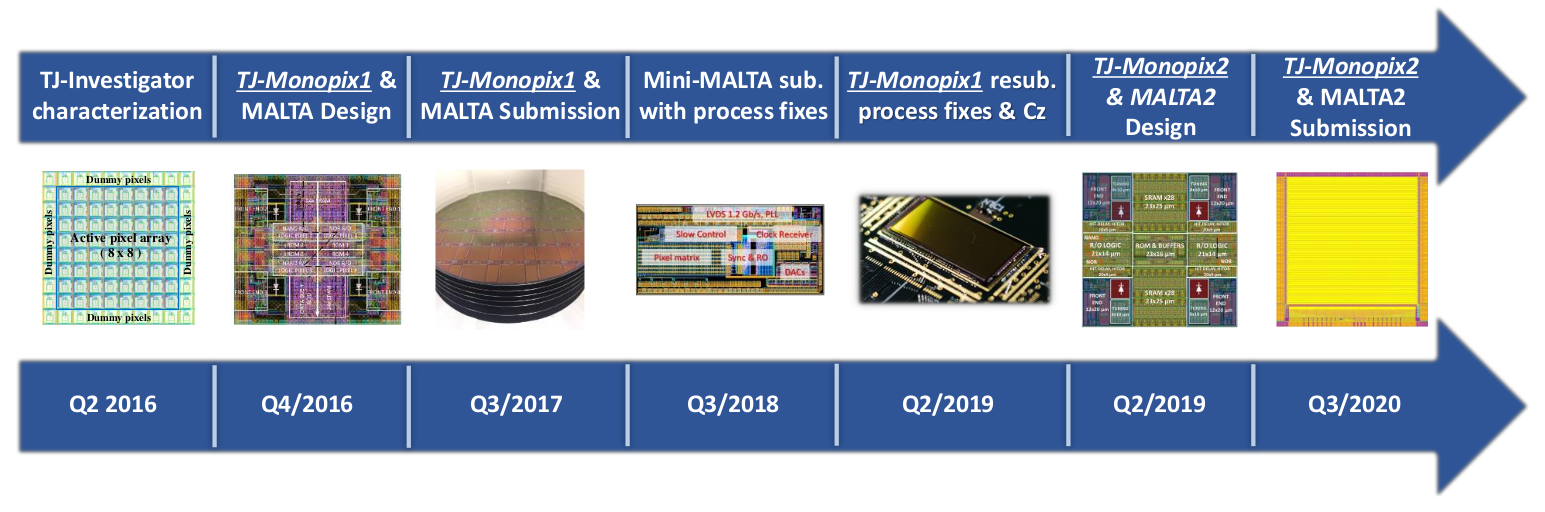
\includegraphics[width=.95\linewidth]{figures/Monopix1/TJ180nm.png}
    \caption{Timeline in TowerJazz productions in 180 nm CMOS imaging process}
    \label{fig:TJ180nm}
\end{figure} 

Another Monopix series, but in 150 nm CMOS technology, has been produced by LFoundry~\cite{LF-Monopix}.
The main differences between the LF-Monopix1 and the TJ-Monopix1 (summarized in table \ref{tab:LF-TJ-Monopix}), lay in the sensor rather than in the readout architecture, as both chips implements a fast column drain R/O with ToT capability \cite{LF-TJ-Monopix-short}\cite{LF-TJ-Monopix-long}.
Concerning the sensors, either are based on a p-type substrate, but with slightly different resistivities; in addition LFoundry pixels are larger, thicker and have a large fill factor (the very deep n-well covers $\sim$55$\%$ of the pixel area). The primary consequence is that LF-Monopix1 pixels have a higher capacity resulting in higher consumption and noise. As I discussed in section \ref{sec:small-large-fill-factor},  the fact that LF-Monopix has a large fill factor electrode is expected to improve its radiation hardness. Indeed, a comparison of the perfomance of the two chips showed that TJ-Monopix suffers a comparatively larger degradation of efficiency after irradiation, due to the low electric field in the pixel corner; on the other hand, a drawback of the large fill factor in LF-Monopix is a significant cross-talk.
\begin{table}
    \begin{center}
    \begin{tabular}{|c | c |c |}
    \hline
    & LF-Monopix1 & TJ-Monopix1\\
    \hline
    \hline
    Resistivity & $>$\SI{2}{k\Omega cm}& $>$\SI{1}{k\Omega cm}\\
    Pixel size & 50  $\times$ 250\si{\um\squared} & 36  $\times$ 40 \si{\um\squared} \\
    Depth & 100-750 \si{\um} & \SI{25}{\um} \\
    Capacity & $\sim$ \SI{400}{fF} & $\sim$ \SI{3}{fF}\\
    Preamplifier & charge & voltage \\
    Threshold trimming & on pixel (4-bit DAC) & global threshold\\
    ToT & 8 bits & 6 bits\\
    Consumption & $\sim$  300\si{mW/cm\squared}& $\sim$  120\si{mW/cm\squared} \\
    Threshold & 1500 $e^-$ & $\sim$ 270 $e^-$ \\
    ENC & 100 $e^-$ & $\sim$ 30 $e^-$\\
    \hline
    \end{tabular}
    \caption{Main characteristics of Monopix1 produced by TowerJazz and LFoundry \cite{LF-TJ-Monopix-short}\cite{LF-TJ-Monopix-long}}
    \label{tab:LF-TJ-Monopix}
    \end{center}
 \end{table}

The TJ-Monopix1 chip contains, apart from the pixels matrix, all the required support blocks used for configuration and testing: 
\begin{itemize}
    \item  the whole matrix contains 224 $\times$ 448 pixels, yielding a total active area approximately equal to \SI{145}{mm\squared} over a total area of 1$\times$2\si{cm\squared};
    \item at the chip periphery are placed some 7-bit Digital to Analog Converter (DAC), used to generate the analog bias voltage and current levels and to confiugure the FE; 
    \item at the EoC is placed a serializer to transferred datas immediately, indeed no trigger memory is implemented in this prototypes;
    \item the matrix power pads are distributed at the sides
    \item four pixels which have analog output and which can be monitored with an oscilloscope, and therefore used for testing
\end{itemize}    
Pixels are grouped in 2$\times$2 cores (fig. \ref{fig:pixels_core}): this layout allows to separate the analog and the digital electronics area in order to reduce the possibile interference between the two parts. In addition it semplifies the routing of data as pixels on double column share the same column-bus to EoC. Therefore pixels can be addressed through the physical column/row or through the logical column/row, as shown in fig. \ref{fig:column_order}: in figure is also highlighted the token propagaion path, whose I will discuss later.

\begin{figure}[h!]
    \begin{subfigure}{.5\textwidth}
    \centering
    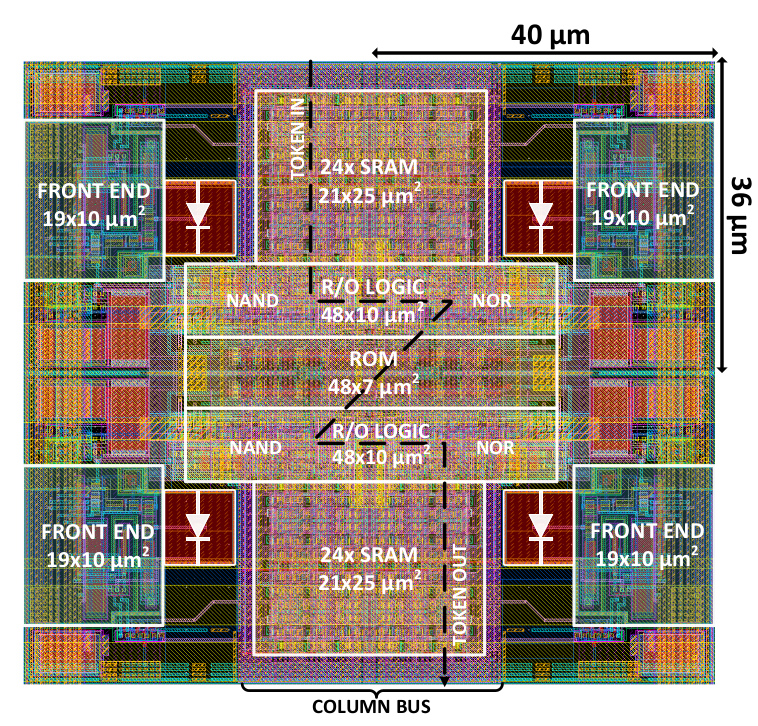
\includegraphics[width=.98\linewidth]{figures/Monopix1/Monopix1_2x2pixelsgroup.png}
    \caption{Layout of a core containing 4 pixels. The analog FE and the digital part are separated in order to reduce cross-talk be}
    \label{fig:pixels_core}
    \end{subfigure}
    \begin{subfigure}{.5\textwidth}
    \centering
    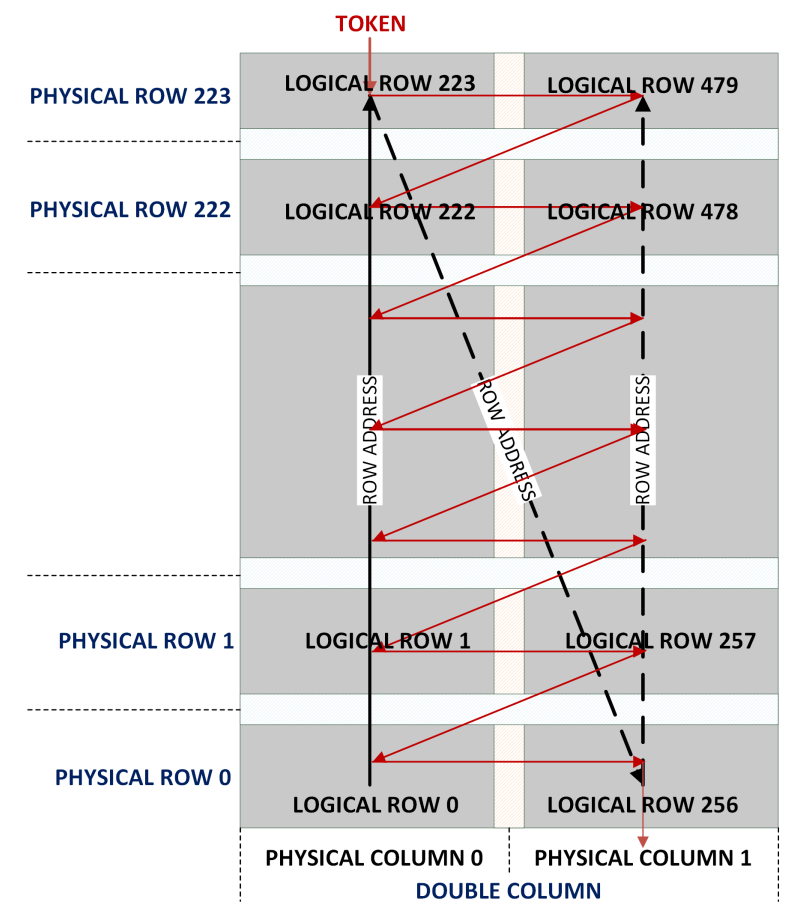
\includegraphics[width=.88\linewidth]{figures/Monopix1/column_order.png}
    \caption{}
    \label{fig:column_order}
    \end{subfigure}
\end{figure}

\begin{table}
    \begin{center}
    \begin{tabular}{| c |c |}
    \hline
    Parameter & Value\\
    \hline
    \hline
    Matrix size &  1$\times$2\si{cm\squared}\\
    Pixel size & 36 $\times$ 40 \si{\um\squared}\\
    Depth & \SI{25}{\um}\\
    Electrode size & \SI{2}{\um}\\
    BCID & \SI{40}{MHz} \\
    ToT-bit & 6 \\
    Power consumption & $\sim$ 120 \si{mW/cm\squared}\\    
    \hline
    \end{tabular}
    \caption{}
    \label{tab:LF-TJ-Monopix}
    \end{center}
\end{table}


\section{The sensor}
    As already anticipated, TJ-Monopix1 has a p-type epitaxial layer and a n doped small collection electrode (\SI{2}{\um} in diameter); to avoid the n-wells housing the PMOS transistors competing for the charge collection, a deep p-well substrate, common to all the pixel FE area, is used.
    TJ-Monopix1 adopts the modification described in section \ref{chap:a_modified_sensor} that allows to achieve a planar depletion region near the electrode applying a relatively small reverse bias voltage.
    This modification improves the efficiency of the detector, especially after irradiation, however a simulation of the electric field in the sensor, made with the software TCAD (Technology Computer Aided Design), shows that a nonuniform field is still produced in the lateral regions of the pixel compromising the efficiency at the corner.
    Two variations to the process have been proposed in order to further enhance the transversal component of electric field at the pixel borders: on a sample of chip, which includes the one in Pisa, a portion of low dose implant has been removed, creating a step discontinuity in the deep p-well corner (fig. \ref{fig:Monopix1_section_scheme}); the second solution proposed\cite{MOUSTAKAS THESYS, PAG 58} consists in adding an extra deep p-well near the pixel edge.
    A side effect of the alteration in the low dose implant is that the separation between the deep p-well and the p-substrate becomes weak to the point that they cannot be biased separately to prevent the punchthrough. 

    \begin{figure}[h!]
        \centering
        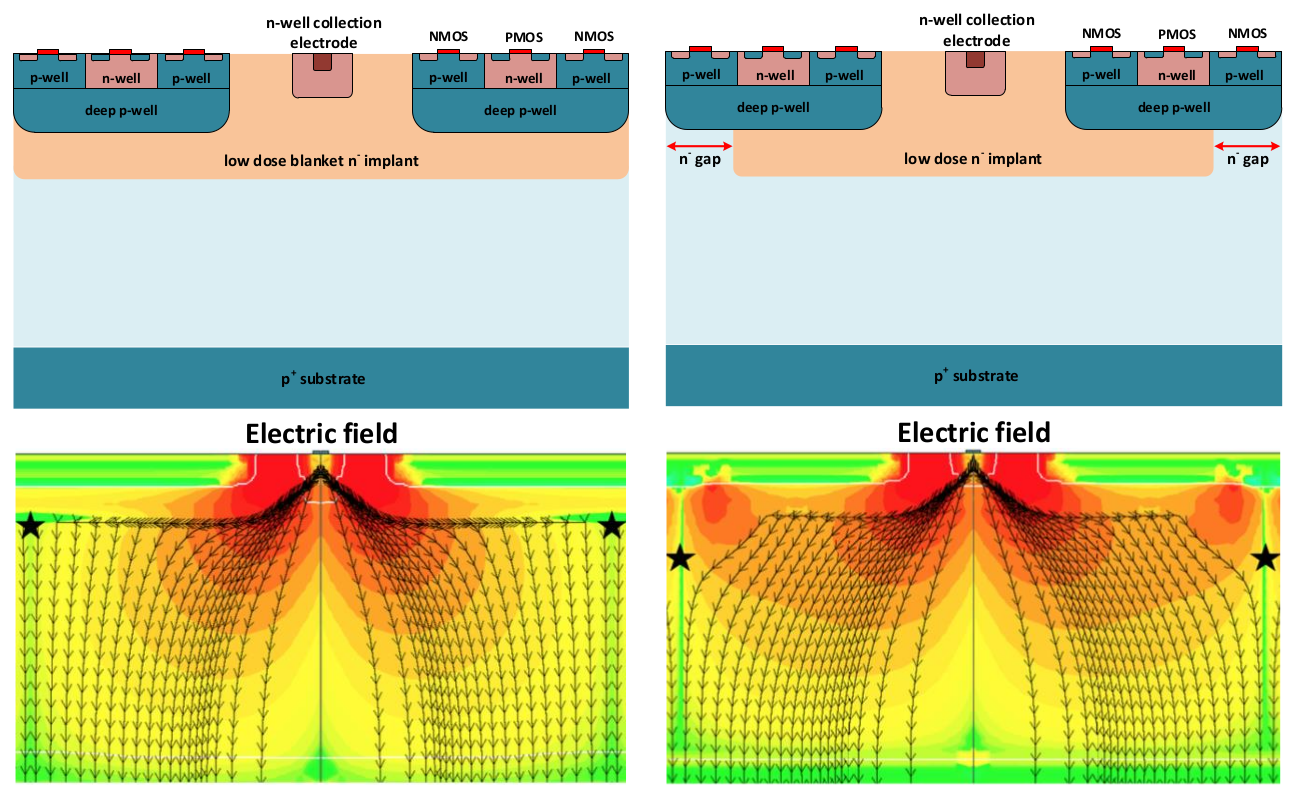
\includegraphics[width=.9\linewidth]{figures/Monopix1/Monopix1_section_scheme.png}
        \caption{(a) The cross-section of a monolithic pixel in the TJ-Monopix with modified process; additionally in (b) a gap in the low dose implant is created to improve the collection of charge due to a bigger lateral component of the electric field. this point in figure  is indicated by a star . transversal component of the electric field drops at the pixel corner}
        \label{fig:Monopix1_section_scheme}
    \end{figure}

    Moreover, to investigate the charge collection properties, pixels within the matrix are split between bottom top half and bottom half and feature a variation in the coverage of the deep p-well: the electronics area can be fully covered or not. In particular the pixels belonging to rows from 0 to 111 are fully covered (FDPW) and pixels belonging to rows from 112 to 223 have a reduced p-well (RDPW), resulting in a enhancement of the lateral component of the electric field.

\section{Front end}
    The matrix is split in four sections, each one corresponding to a different flavor of the FE. The four variation have been implemented in order to test the data-bus readout circuits and the input reset modes.
    \begin{figure}[h!]
        \centering
        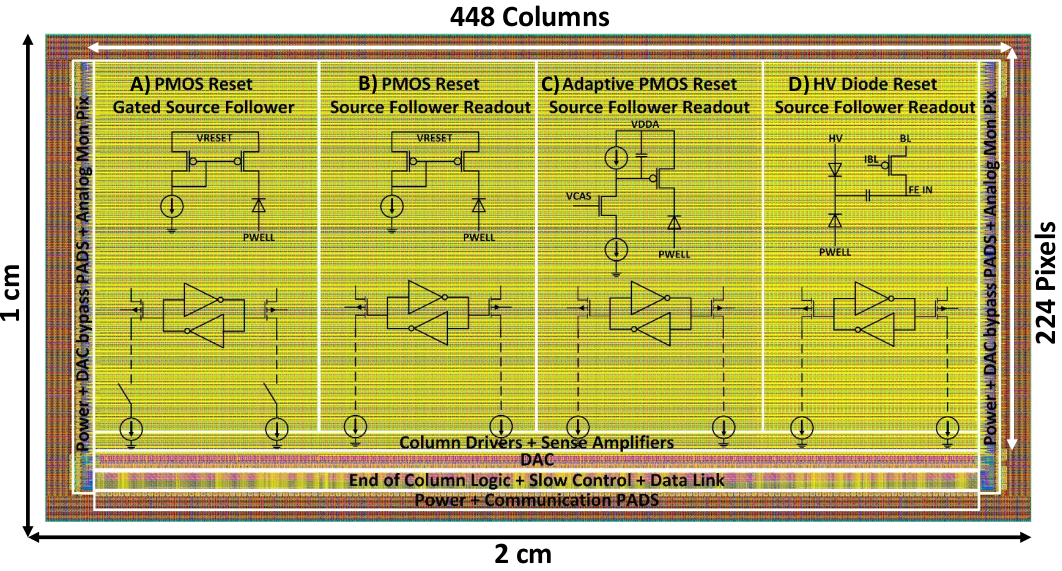
\includegraphics[width=.8\linewidth]{figures/Monopix1/Monopix1_flavors.png}
        \caption{}
        \label{fig:Monopix1_flavors}
    \end{figure}

    All the flavors implement a source-follower double-column bus readout: the standard variation is the flavor B, that features a PMOS input reset (refered as "PMOS reset"). Flavor A is identical to flavor B except for the realization of the source follower (it is a gated one) that aim to reduce the power consumption.\red{cosa significa?} C instead implements a novel leakage compensation circuit.
    Moreover the collection electrode in flavors A, B, C is DC-coupled to the front-end input, while in D is AC-coupled, providing to applu a high bias voltage; for this reason flavor D il called "HV flavor".

    \red{Principio generale: R resistenza di reset deve essere abbastanza grande in modo da far si che il ritorno allo zero è abbastanza lento (non devi "interferire" con la tot slope e non deve essere più corto del tempo del preamplificatore, sennò hai perdita di segnale).
    Baseline reset: all'input solitamente hai un PMOSS o un diodo;  
    R reset}

    \subsection{ALPIDE-like}
        ALPIDE chips, developed by the ALICE collaboration, implemented a standard FE to the point that many CMOS MAPS detectors used a similar FE and are called "ALIPDE-like". 
        Concidering that both TJ-Monopix1 and ARCADIA-MD1 have an ALPIDE-like FE, I am going to explain the broad principles of the early FE stage. 
        \begin{figure}[h!]
            \begin{subfigure}{.5\textwidth}
            \centering
            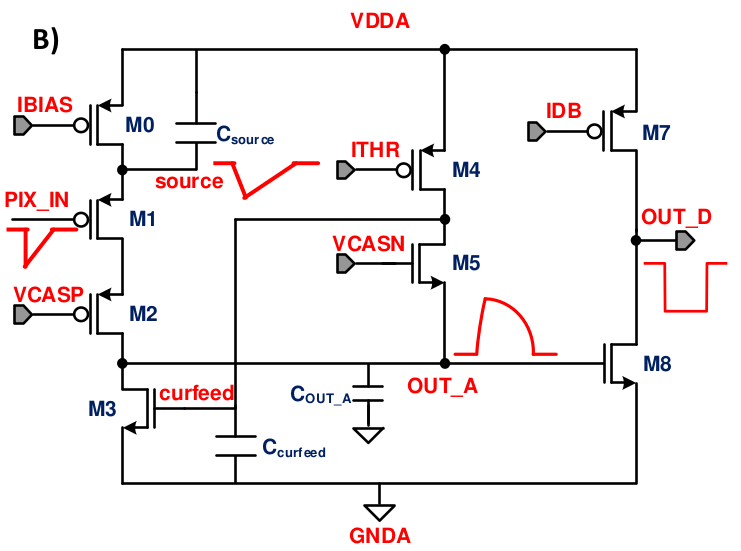
\includegraphics[width=.98\linewidth]{figures/Monopix1/ALPIDE_FE.png}
            \caption{ALPIDE-like}
            \label{fig:ALPIDE-like}
            \end{subfigure}
            \begin{subfigure}{.5\textwidth}
            \centering
            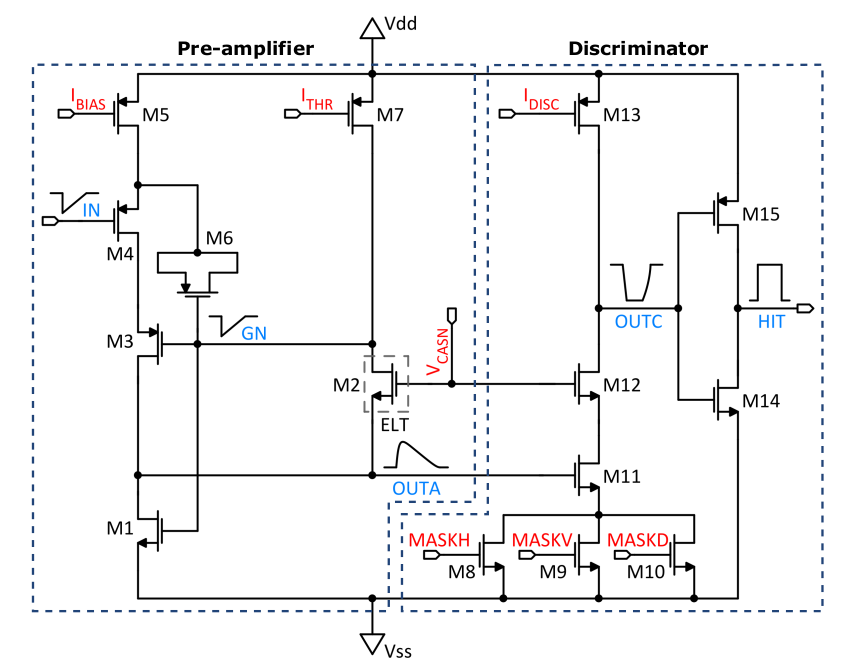
\includegraphics[width=.98\linewidth]{figures/Monopix1/Monopix1_FE_circuit.png}
            \caption{}
            \label{fig:Monopix1_FE_circuit}
            \end{subfigure}
        \end{figure}
        The general idea is of the amplification to transfer the charge from a bigger capacity\cite{ALPIDE-FE}, $C_{source}$, to a smaller one, $C_{out}$: the input transistor M1 with current source IBIAS acts as a source follower and this forces the source of M1 to be equal to the gate input  $\Delta V_{PIX\_IN} = Q_{IN}/C_{IN}$.
        \begin{equation}
            Q_{source} = C_{source} \Delta V_{PIX\_IN}
        \end{equation}
        The current in M2 and the charge accumulates on $C_{out}$ is fixed by the one on $C_{source}$:
        \begin{equation}
            \Delta V_{OUT\_A} = \frac{Q_{source}}{C_{OUT\_A}} = \frac{C_{source}\Delta V_{PIX\_IN}}{C_{OUT\_A}}  = \frac{C_{Source}}{C_{OUT\_A}}\frac{Q_{IN}}{C_{IN}}
        \end{equation}
        A second branch (M4, M5) is used to generate a low frequency feedback, where VCASN and ITHR set the baseline value of the signal on $C_{OUT\_A}$ and the velocity to goes down to the baseline.\\
        \red{IL RUOLO DI CURVFEED NON L'HO CAPITO.}\\
        Finally IDB defines the charge threshold with which the signal $OUT\_A$ must be compared: depending on if the signal is higher than the threshold or not, the $OUT\_D$ is high or low respectively.

        The actual circuit implemented in TJ-Monopix1 is shown in figure \ref{fig:Monopix1_FE_circuit}: the principal difference lays in the addition of disableing pixels' readout. This possibility is uttermost important in order to reduce the hit rate and to avoid saturating the bandwidth due to the noisy pixels, which typically are those with manufacturing defects.
        In the circuit transistors M8, M9 and M10 have the function of disabling registers with coordinates MASKH, MASKV and MASKD (respectivelly vertical, orizontal and diagonal) from readout: if all three transistors-signals are low, the pixel's discriminator is disabled. 
        Compared with a configurable masking register which would allow disableing pixels individually, to use a triple redundancy reduces the sensistivity to SEU but also gives amount of intentionally masked ("ghost") pixels.
        This approach is suitable only for extremely small number N of pixel has to be masked: if two coordinate projection scheme had been implemented, the number of ghost pixels would have scale with $N^2$, if instead three coordinates are used, the N's exponential is lower than 2 (fig. \ref{fig:masking_scheme})
        \begin{figure}[h!]
            \centering
            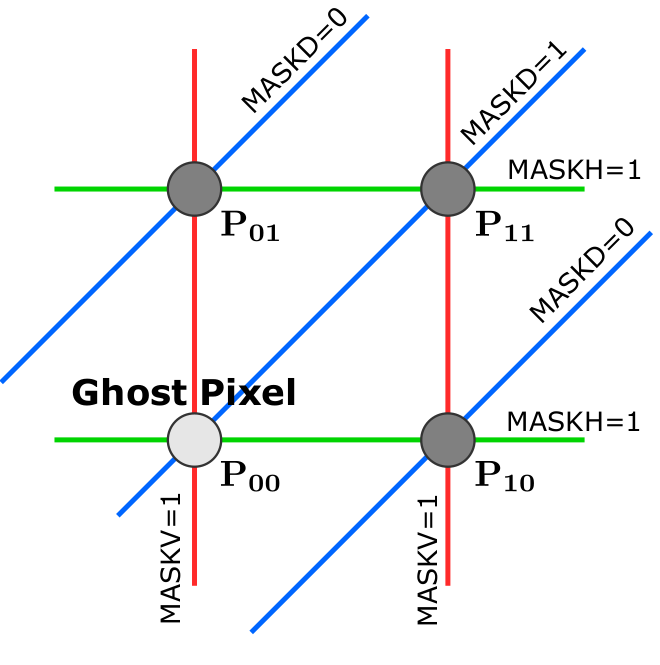
\includegraphics[width=.3\linewidth]{figures/Monopix1/masking_scheme.png}
            \caption{}
            \label{fig:masking_scheme}
        \end{figure}

        \begin{table}
            \begin{center}
            \begin{tabular}{|c | c | c |}
            \hline
            Parameter & Meaning & \\
            \hline
            \hline
            IBIAS & mainly controls the rise time & \red{yes? check}\\
            IDB & sets the discriminator threshold & yes\\
            ITHR & sets the velocity of the return to the baseline & yes \\
            ICASN & sets the baseline of the signal & yes\\
            VRESET & sets the gain of the preamplifier & yes\\
            IRESET & sets the gain of the preamplifier & no\\
            \hline
            \end{tabular}
            \caption{FE parameters which must be setted through the DAQ. "Function" means that higher parameter implies higher value}
            \label{tab:FE-parameters}
            \end{center}
        \end{table}
    


\section{Readout logic}
    TJ-Monopix1 has a triggerless, fast and with ToT capability R/O which is based on a column-drain architecture.      
    On the pixel are located two Random Access Memory (RAM) cells to store the 6-bit LE and 6-bit TE of the pulse, and a Read-Only Memory (ROM) containing the 9-bit pixel address. Excluded these memories, TJ-Monopix1 hasn't any other buffer: if a hit arrives while the pixel is already storing a previous one, the new data get lost.  
    After being read, the data packet is sent to the EoC periphery of the matrix, where a serializer transfers it off-chip to an FPGA (\ref{fig:R/O-system}). There a FIFO is used to temporarily stored the data, which is transmitted to a computer through an ethernet cable in a later time.  
    \begin{figure}
        \begin{subfigure}{\textwidth}
        \centering
        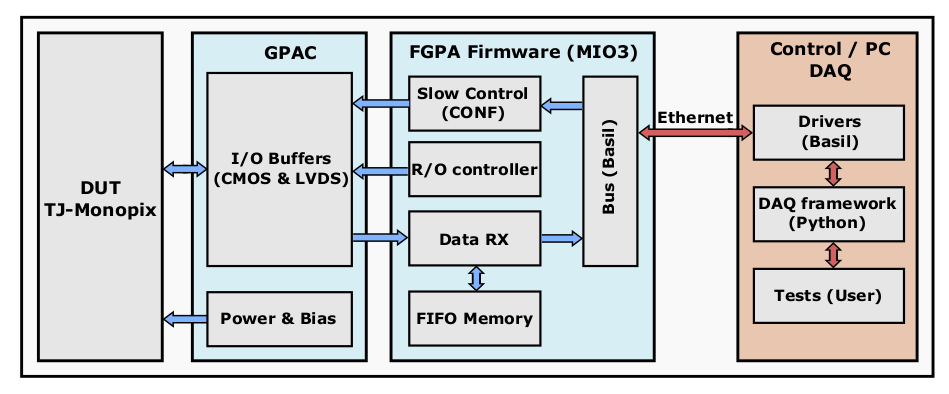
\includegraphics[clip,width=0.8\linewidth]{figures/Monopix1/schematic_boards.png}
        \end{subfigure}
        \bigskip
        \begin{subfigure}{\textwidth}
        \centering    
        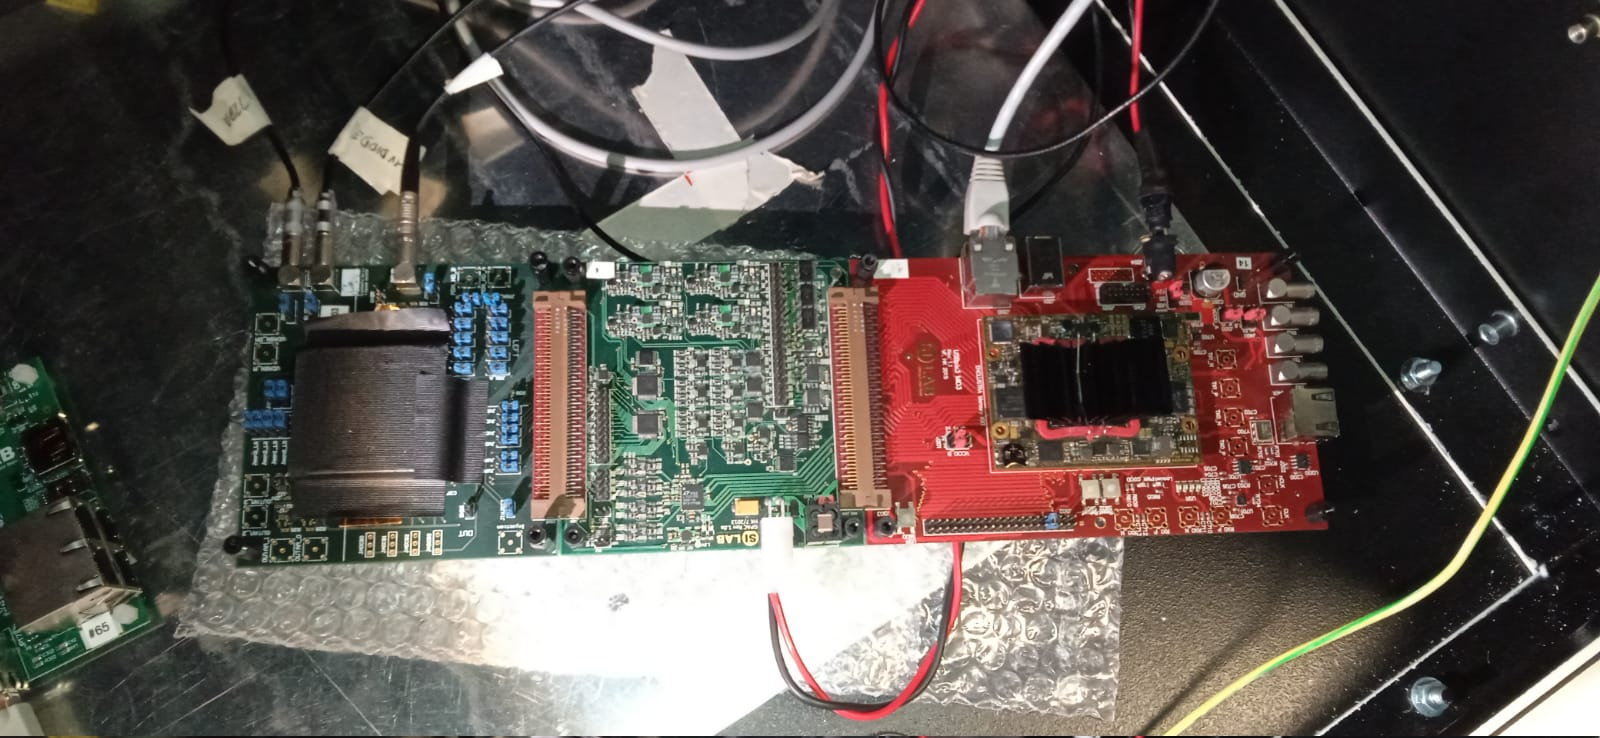
\includegraphics[clip,width=0.8\linewidth]{figures/Monopix1/monopix1_front.jpeg}
        \end{subfigure}
        \caption{Main caption}
        \label{fig:R/O-system}
    \end{figure}


    The access to the pixels' memory and the transmission of the data to the EoC, following a priority chain, is managed by control signals and is based on a Finite State Machine (FSM) composed by four state: no-operation (NOP), freeze (FRZ), read (RD) and data transfer (DTA). The readout sequence (\ref{fig:readout_schematics}) starts with the TE of a pulse: the pixel immediately tries to grab the column-bus turning up a hit flag signal called \textit{token}.   
    The token is used to control the priority chain and propagates across the column indicating what pixel that must be read. To start the readout and avoid that the arrival of new hits disrupt the priority logic, a \textit{freeze} signal is activated, and then a \textit{read} signal controls the readout and the access to memory.
    During the freeze, the state of the token for all pixels on the matrix remains settled: this does not forbid new hits on other pixels from being recorded, but forbids pixels hit from turning on the token until the freeze is ended. 
    The freeze stays on until the token covers the whole priority chain and gets the EoC: during that time new token cannot be turned on, and all hits arrived during a freeze will turn on their token at the end of the previous freeze.  
    Since the start of the token is used to assign a timestamp to the hit, the token time has a direct impact on the time resolution measurement; this could be a problem coping with high hits rate. 
    \begin{figure}[h!]
        \centering
        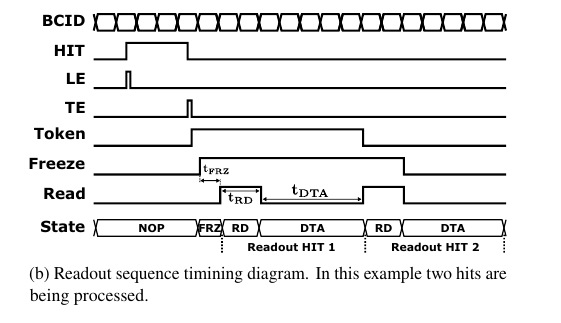
\includegraphics[width=.5\linewidth]{figures/Monopix1/readout_timing.png}
        \caption{Readout timing diagram: in this example two hits are being processed}
        \label{fig:readout_timing}
    \end{figure}

    The analog FE circuit and the pixel control logic are connected by an edge detector which is used to determine the LE and the TE of the hit pulse(fig. \ref{fig:pixel_logic}): when the TE is stored in the first latch the edge detector is disabled and, if the \textcolor{red}{FREEZE} signal is not set yet, the readout starts. 
    At this point the HIT flag is set in a second latch and a token signal is produced and depending on the value of \textcolor{Cerulean}{Token in} the pixel can be read or must wait until the \textcolor{Cerulean}{Token in} is off. In figure an OR is used to manage the token propagation, but since a native OR logic port cannot be implemented with CMOS logic, a sum of a NOR and of an inverter is actually used; this construct significantly increases the propagation delay (the timing dispersion along a column of 0.1-0.2 ns) of the token and to speed up the circuit optimized solution are often implemented.  
    When the pixel become the next to be read in the queue, and at the rising edge of the \textcolor{red}{READ} signal, the state of the pixel is stored in a D-latch and the pixel is allowed to use the data bus; the TE and the HIT flag latches are reset and a \textcolor{Cerulean}{READINT} signal that enable access of the RAM and ROM cells is produced.\\
    \begin{figure}[h!]
        \centering
        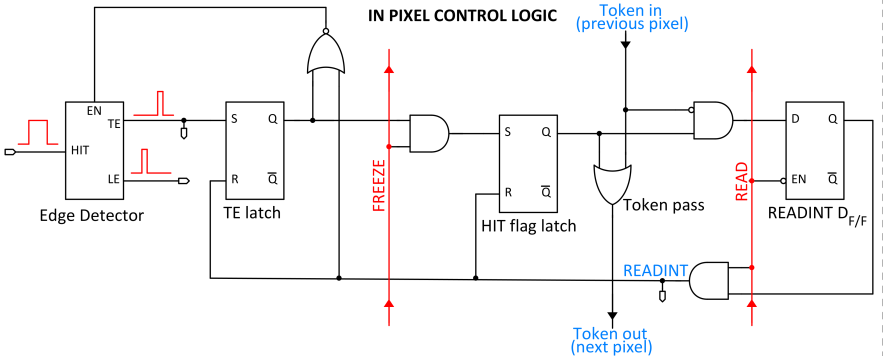
\includegraphics[width=.9\linewidth]{figures/Monopix1/Monopix1_readout_schematics.png}
        \caption{}
        \label{fig:pixel_logic}
    \end{figure}
    
    The final data must provide all the hits' information: the pixel address, the ToT and the timestamp. All those parts are assigned and appended at different time during the R/O chain:  
    \begin{itemize}
        \item\textbf{Pixel address:} while the double column address (6-bit) is appended by the EoC circuit, the row address (8-bits for each flavor) and the physical column in the doublet (1-bit) are assigned by the in-pixel logic      
        \item \textbf{ToT:} is obtained offline from the difference of 6-bits TE and 6-bits LE, stored by the edge detector in-pixel; since a 40 MHz BCID is distributed across the matrix, the ToT value is range 0-64 clock cycle which corresponds to 0-1.6 \si{\us}  
        \item \textbf{Timestamp:} The timestamp of the hit correspond to the time when the pixel set up the token; it is assigned by the FPGA, that uses the LE, TE and a 640 MHz clock to derive it. For all those hits which arrived while the matrix is frozen, the timestamp is no more correlated with the time of arrival of the particle         
    \end{itemize}
    When the bits are joined up together the complete hit data packet is 27-bit. 

    \subsection{Dead time measurements}
        The hit loss is due to analog and digital pile up: the first one occurs when a new hit arrives during the pre-amplifier response, the second instead, which is the more relevant contribution with high rate, while the information of the previous hit has not yet been transferred to the periphery.  
        As only one hit at a time can be stored on the pixel's RAM, until the data have completed the path to get out, the pixel is paralyzed and the dead time $\tau$ almost corresponds with the time needed to trasmit the data-packets off-chip.
        Since the exportation of data from pixel to the EoC occurs via a 21-bits data bus, only one clock cycle is need to transfer the data to the end of column and the dead time bottleneck is given by the bandwidth of the serializer at the EoC. In our setup the serializer operates at 40 MHz, thus to transmit a data packet (27-bit considering the addition at the EoC) at least \SI{675}{ns} are needed. 
        For what we have said so far, the R/O is completely sequential and therefore is expected a linear dependence of the reading time on the number of pixels to read:
        \begin{equation}
            \tau =\, 25\: \unit{ns}\, \times\, (\alpha\, N +\, \beta)
            \label{eq:reading_time}
        \end{equation}
        where $\alpha$ and $\beta$ are parameters dependent on the readout chain setting. 
        
        To measure and test the linearity of the reading time with the number of pixels firing, I have used the injection mode available on the chip. 
        Indeed, the injection mode allows fixing not only the amplitude of the pulse, which corresponds to the charge in DAC units, but also the period and the width.
        I have injected a fix number of pulses (100) and looked for the rate when the efficiency decreases. 
        Moreover to test that there is no dependece of the digital readout time from the charge of the pulse, I have try to change the amplitude of the pulse injected, but the parameters found were consistent with the default configuration ones.

        \red{Al posto degli esempi con 5 e 10 pixels metterei un esempio dell'efficienza vs il periodo quando leggo un singolo pixel. Una cosa che volevo fare era anche provare a fittare la slope con cui l'efficienza scende: se la slope è uguale per tutti il readout diventa completamente predittivo. }
        \begin{figure}[h!]
            \begin{subfigure}{.5\textwidth}
            \centering
            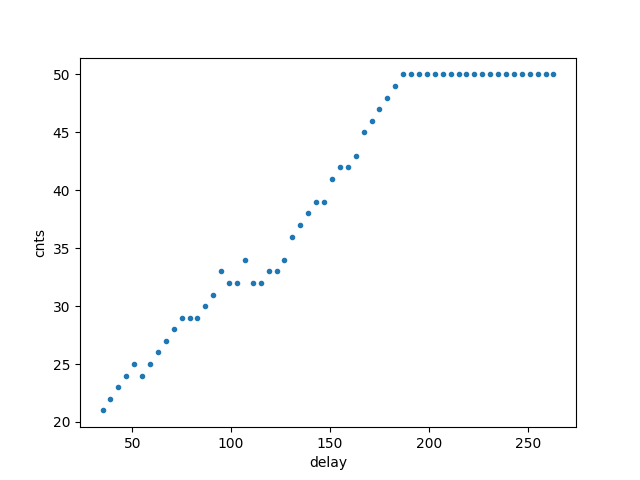
\includegraphics[width=.98\linewidth]{figures/Monopix1/efficiency_5pixels.png}
            \caption{\red{efficiency vs DELAY 5 pixels}}
            \label{fig:}
            \end{subfigure}
            \begin{subfigure}{.5\textwidth}
            \centering
            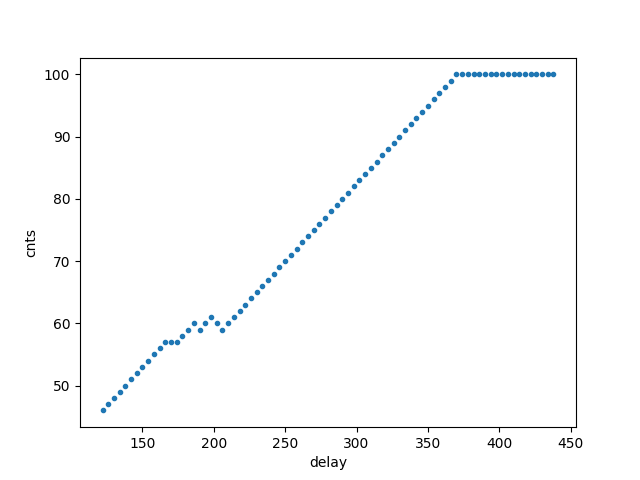
\includegraphics[width=.98\linewidth]{figures/Monopix1/efficiency_10pixels.png}
            \caption{\red{efficiency vs DELAY per 10pixels}}
            \label{fig:}
            \end{subfigure}
        \end{figure}
        
        While the single pixel reading time and the dead time do not depend on the position on the pixel matrix and are equal to \red{106 (46+60)} clock counts within 1 clock count, on the other hand the $\tau$ depends on the pixel position on the matrix when more than one pixel are firing. 
        In particular the priority chain goes from row 224 to row 0, and from col 0 to 112, that means the last pixels to be read is the one on le bottom right corner of the matrix. 

        In figure \ref{fig:dead_time} is reported the reading time versus the number of pixels injected; the R/O parameters that control the reading time and their default values are reported on table \ref{tab:tab:R/O_param}.
        \begin{table}
            \begin{center}
            \begin{tabular}{|c | c | c |}
            \hline
            Parameter & Value [\si{DAC}] & Value [\si{\us}]\\
            \hline
            \hline
            START\_FREEZE & 64 & 1.6\\
            STOP\_FREEZE & 100 & 2.5\\
            START\_READ & 66 & 1.65\\
            STOP\_READ & 68 & 1.7\\
            \hline
            \end{tabular}
            \caption{Default configuation of the R/O parameters}
            \label{tab:R/O_param}
            \end{center}
        \end{table}

        The factor $\alpha$, referring to eq. \ref{eq:reading_time} is proportional to the difference (STOP\_FREEZE - START\_READ), while the offset $\beta$ lies between 5 and 15 clock counts.
        Since through the injection a random hit rate on the matrix can't be simulated, as the coordinates of the pixels to inject must be specified, for convenience I used the pixels on the same column/row. No difference in the $\alpha$ and $\beta$ coefficients has been observed between the two case. 
        \begin{figure}[h!]
            \centering
            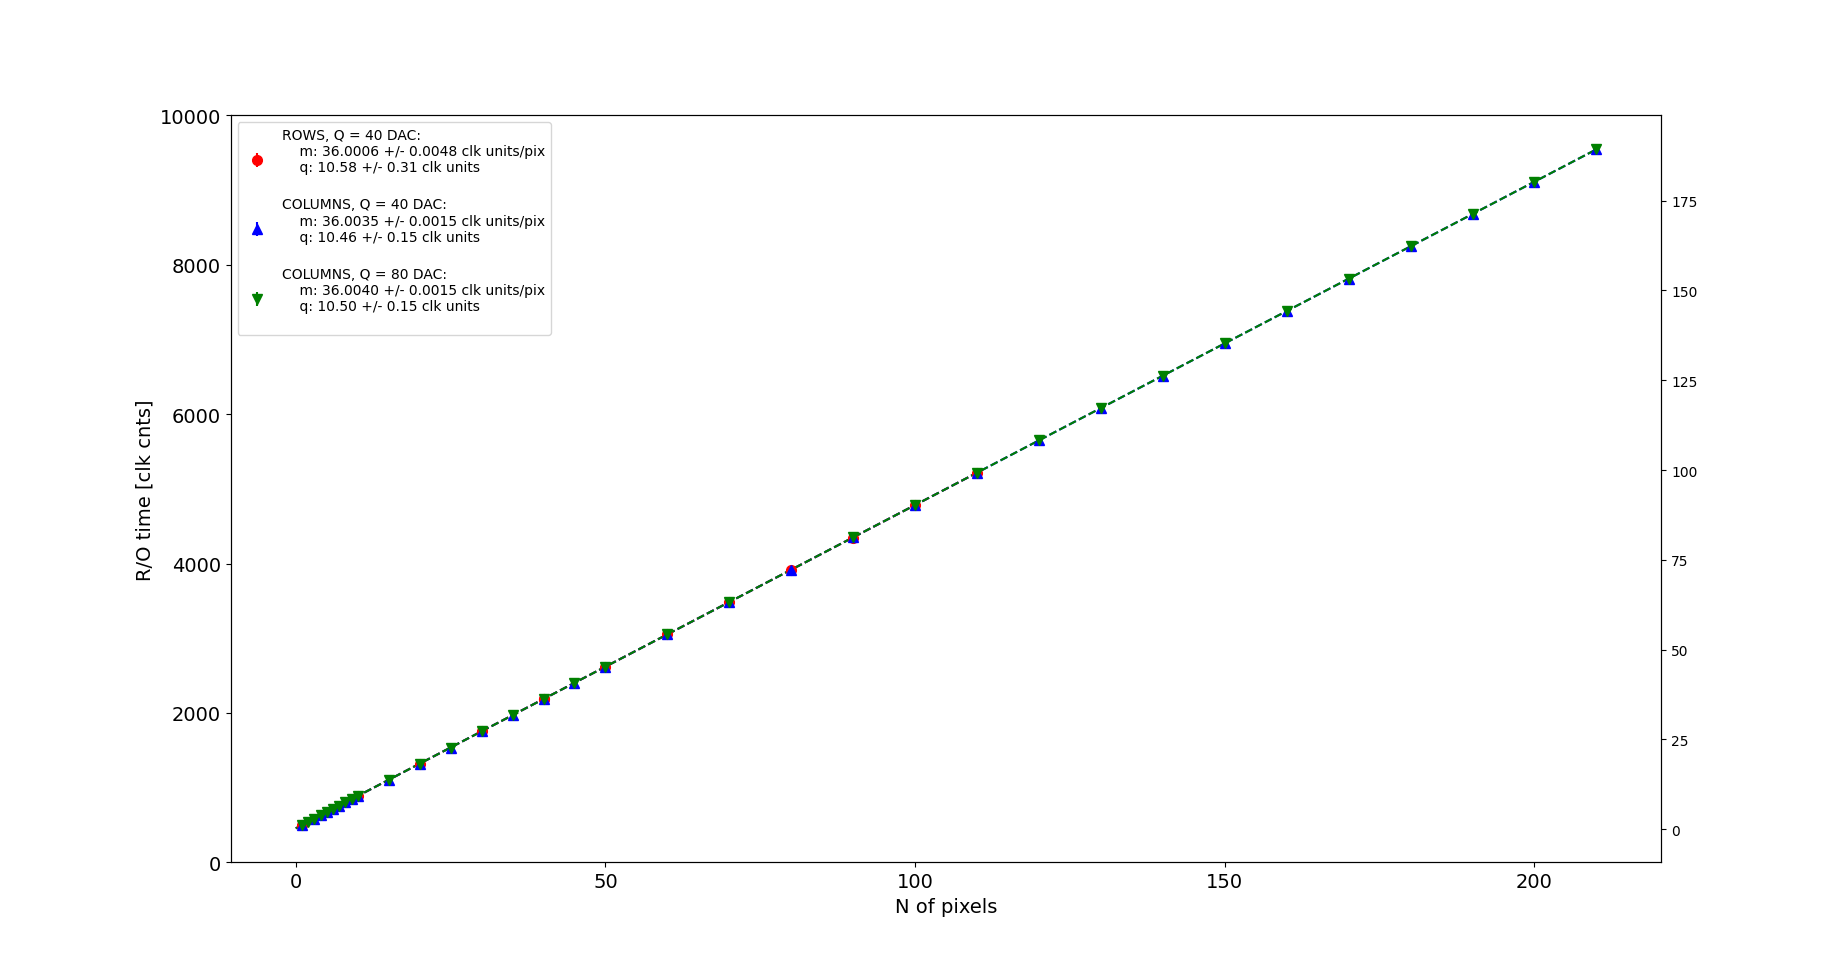
\includegraphics[width=.9\linewidth]{figures/Monopix1/default_line.png}
            \caption{}
            \label{fig:dead_time}
        \end{figure}

        \begin{figure}[h!]
            \centering
            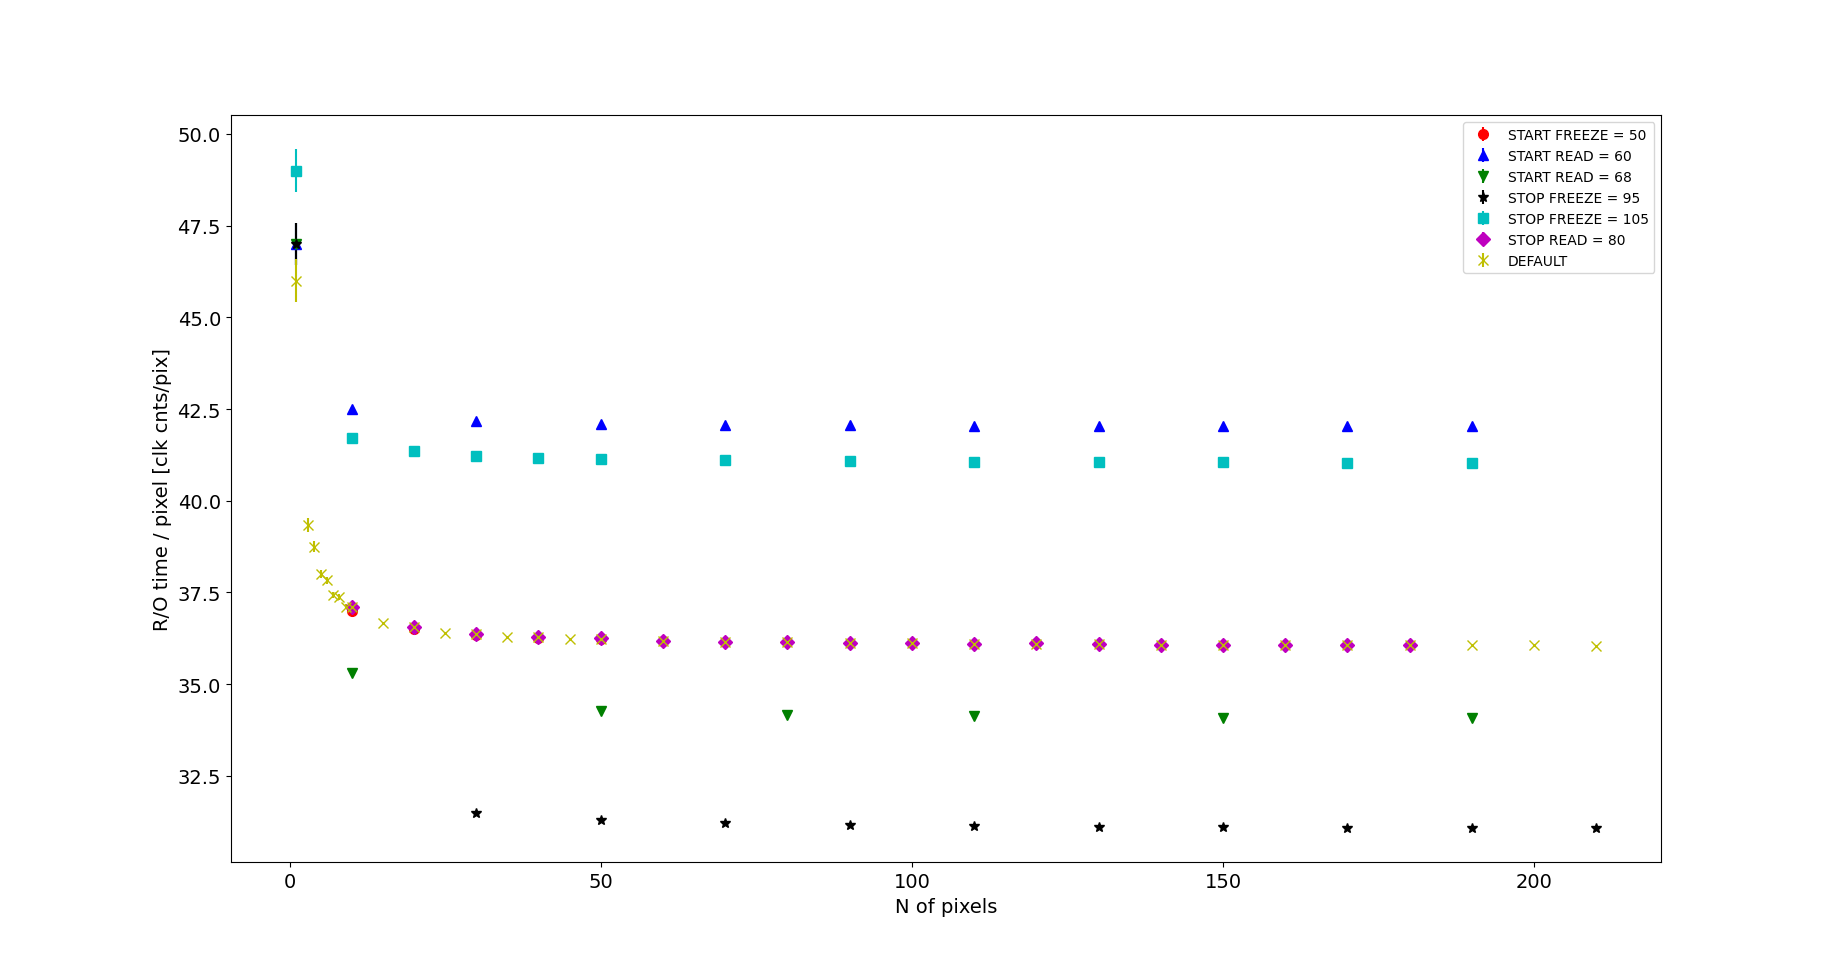
\includegraphics[width=.9\linewidth]{figures/Monopix1/parameters_points.png}
            \caption{}
            \label{fig:dead_time}
        \end{figure}        

        \red{Ci sarebbe da spiegare perchè i parametri che usiamo noi come default non sono quelli che minimizzano il tempo di lettura. La spiegazione è che "Abbiamo copiato i valori dal repositorio di quelli di Bonn". Un'altra domanda potrebbe essere: come mai non ho esplorato una zona più vasta per i parametri del R/O. Cambiando molto i parametri del R/O la lettura non funzionava per niente: ad esempio CONF\_STOP\_FREEZE non può essere impostato nè sopra 105 nè sotto 95}


\section{Measurements with radioactive sources}
    \red{CI metterei i plot con ferro, stronzio e cosmici}
    Istogrammi, cluster distribution e definizione di cluster, coincidenze casuali con rumore. 

\section{Calibration of the ToT signal}
    \red{calibrazione con il ferro}
    Ci metterei un'istogramma del


\cite{ARCADIA-Pancheri}
\cite{ARCADIA-Pancheri2}

Breve introduzione analoga a Monopix1 in cui descrivo brevemente la "timeline" da SEED Matisse a Md1 e Md2

\section{The sensor}
    ARCADIA-MD1 is an LFoundry chip which implements the technology 110 nm CMOSS node
    with six metal layer \ref{articolo fully depl}.
    The standard p-type substrate was replaced with an n-type floating zone material,
    that is a tecnique to produce purified silicon crystal. (pag 299 K.W.).\\
    \begin{figure}[h!]
        \centering
        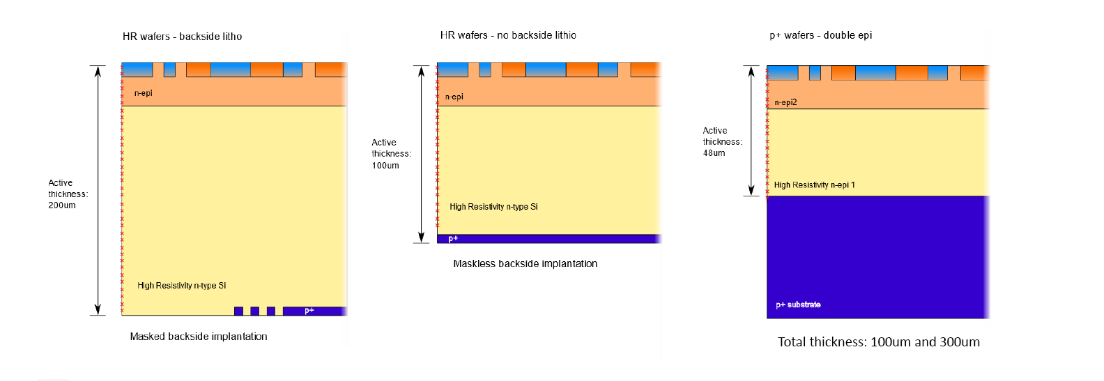
\includegraphics[width=.8\linewidth]{figures/ARCADIA/ARCADIA_substrate.png}
        \caption{}
        \label{fig:ARCADIA_substrate}
    \end{figure}

    Wafer thinning and backside litography were necessary to introduce a junction
    at the bottom surface, used to bias the substrate to full depletion while
    maintaining a low voltage at the front side.  \\
    C'è un deep pwell per - priority chainseparare l'elettronica dal sensore; per controllare il punchthought
    è stato aggiunto un n doped epitaxial layer having a resistivity lower than the substrate.



    It is part of the cathegory of DMAPS
    Small electrode to enhance the signal to noise ratio.

    It is operated in full depletion with fast charge collection by drift.

    Prima SEED si occupa di studiare le prestazioni: oncept study with small-scale test structure (SEED),
    dopo arcadia: technology demonstration with large area sensors
    Small scale demo SEED(sensor with embedded electronic developement)
    Quanto spazio dato all'elettronica sopra il pwell e quanto al diodo. ..

\section{Readout logic and data structure}
    \subsection{Matrix division and data-packets}
        The matrix is divided into an internal physical and logical hierarchy:
        The 512 columns are divided in 16 section: each section has different voltage-bias + serializzatori.
        Each section is devided in cores () in modo che in ogni doppia colonna ci siano 1Pacchetto dei dati
        6 cores. ricordati dei serializzaatori: sono 16 ma possono essere ridotti ad uno in modalità spazio
        \begin{figure}[h!]
            \centering
            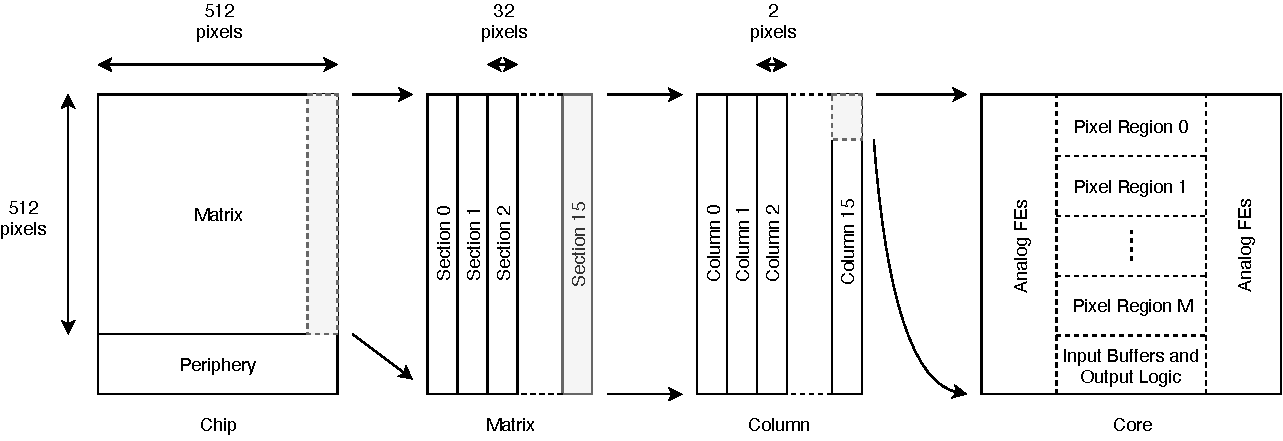
\includegraphics[width=.95\linewidth]{figures/ARCADIA/hierarchy.pdf}
            \caption{}
            \label{fig:hierarchy}
        \end{figure}

        
        \begin{figure}[h!]
            \centering
            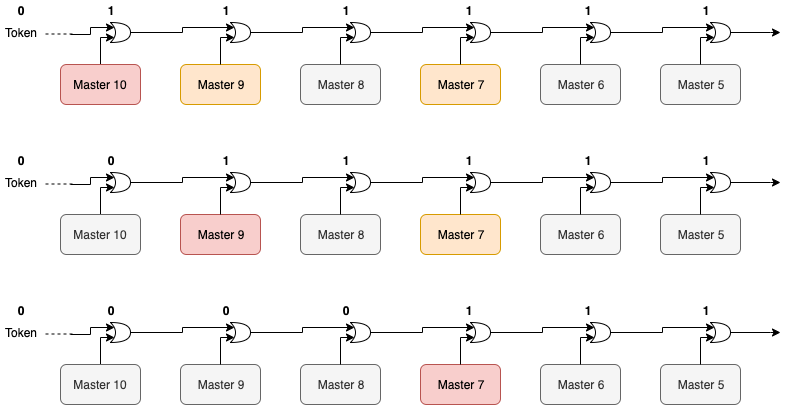
\includegraphics[width=.95\linewidth]{figures/ARCADIA/token_chain.png}
            \caption{}
            \label{fig:token_chain}
        \end{figure}


        \begin{figure}[h!]
            \centering
            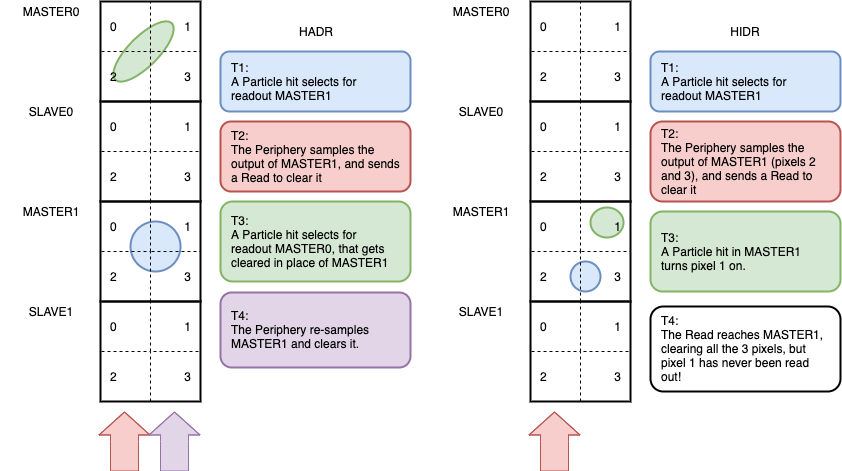
\includegraphics[width=.95\linewidth]{figures/ARCADIA/hadrhidr.png}
            \caption{}
            \label{fig:hadrhidr}
        \end{figure}
        


        \begin{figure}[h!]
            \centering
            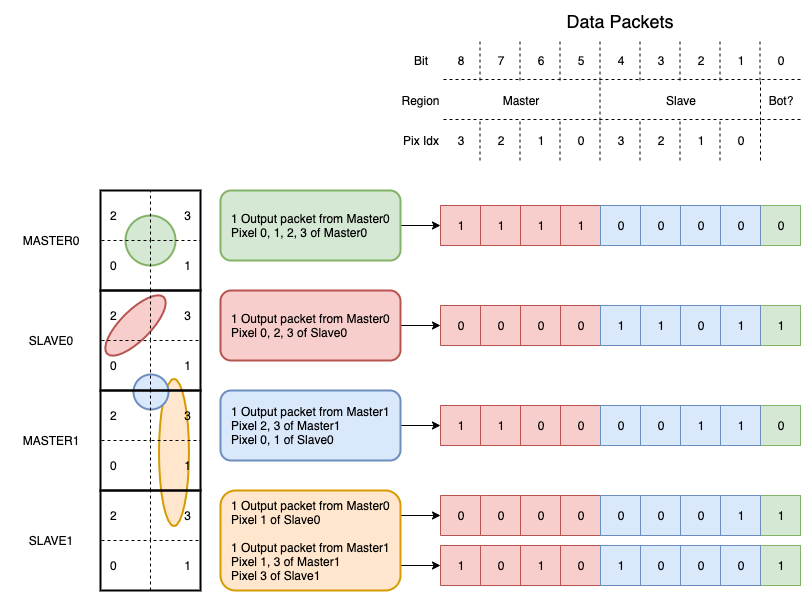
\includegraphics[width=.95\linewidth]{figures/ARCADIA/clustering.png}
            \caption{}
            \label{fig:clustering}
        \end{figure}

        \begin{figure}[h!]
            \centering
            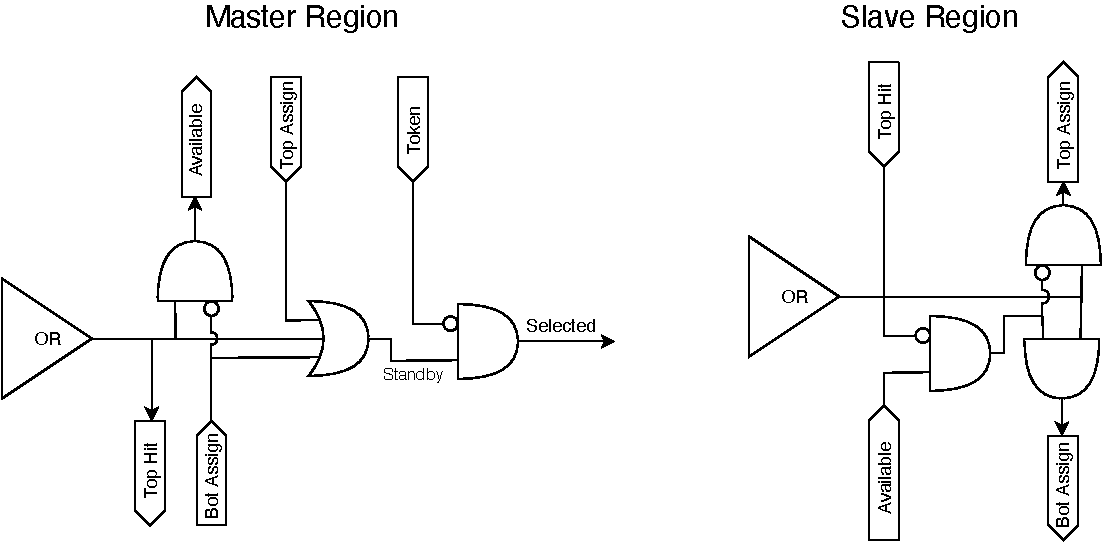
\includegraphics[width=.95\linewidth]{figures/ARCADIA/clustering_logic.pdf}
            \caption{}
            \label{fig:clustering_logic}
        \end{figure}
        


        Questa divisione si rispecchia in come sono fatti i dati: scrivi da quanti bit un
        dato è fatto e le varie cordinate che ci si trovano dentro; devi dire che c'è un pixel hot
        e spieghi dopo a cosa serve, e devi accennare al timestamp

        "A core is simply the smallest stepped and repeated instance of digital circuitry.
        A relatively large core allows one to take full advantage of digital sybthesis tools
        to implement complex functionality in the pixel matrix, sharing resources among
        many pixels as needed.".
        pagina 28 della review.\\



        TABELLA: con la gerarchia del chip
        Matrix (512x512 pixels)
        Section (512x32 pixels)
        Column (512x2)
        Core (32x2)
        Region (4x2)

        Nel chip trovi diverse padframe: cosa c'è nelle padframe e End of section.

        "DC-balance avoids low frequencies by guaranteeing at least one transition every
        n bits; for example 8b10b encoding n =5"



\chapter{Characterization}
%    \red{Measurement of the magnitude of the collected charge has also been generally available for pixel detectors, and has been used to improve the 3D space point precision through interpolation as well as for particle identification through specific ionization measurement.
\red{\begin{itemize}
    \item rifai il conto della lunghezza di attenuazione. Ho trovato (presentazione Luciano Mus) 29 um per ka e 37 um per kb. 
    \item Con il PMOS la configurazione del FE di default è: e richiama i significati delle variabili. 
    \item parla dell HV
\end{itemize}}

\section{TJ-Monopix1 characterization}
    \subsection{Threshold and noise: figure of merit for pixel detectors}
        %python3 -i calibration/scurve_tot_histo.py -f calibration/calibration_data/20220506 -i 1 100 questo script crea i file di output contenenti i gli istogrammi del tot e della s curve
        %python3 -i calibration/tot_charge_plotting.py -f calibration/calibration_data/20220506 per fare il plot della s curve e relativi residui 
        %python3 -i calibration/tot_histo2d.py -f calibration/calibration_data/PMOS/20220506 per fare l'istogramma 2d del tot           
        A characterization of threshold and noise is typically necessary since these values have an impact on the operating conditions and on the performance of the chips, so much that the signal to threshold ratio may be considered as the figure of merit for pixel detectors rather than the signal to noise ratio.
        The mean minimum stable threshold evolved through different generation of chips: in the 1st generation it was around \SI{2500}{e-} while in the 3rd (corresponding to nowadays chips) is less than \SI{500}{e-}. This allows in thinner sensors with smaller signals: from \SI{16000}{e-} produced in \SI{200}{\um}, the signal expected moved down to \SI{2000}{e-} produced in \SI{25}{\um}. According with this, the threshold of TJ-Monopix1 is around \SI{500}{e-}.
 
        Obviously the threshold has to be located between the noise peak around the baseline and the signal distribution, in particular it has to be low enough to mantain a high signal efficiency, but also high enough to cut the noise: for a low threshold many pixels can fire at the same time and a positive feedback can set off a chain reaction eventually, causing all the other pixels to fire.
        Thus, the noise sets a lower bound to the threshold: if an occupancy $\leqslant$ $10^{-4}$ is required, for example, this correspond to the Gaussian 1-sided tail fraction for \SI{3.7}{\sigma}.
        In this case, if the noise is \SI{100}{e-} (resonable), the threshold must be higher than \SI[parse-numbers=false]{3.7\times100}{e-}.
        Typically this argument sets only a minimal bound to the threshold since the variation with time and from pixel to pixel have to be taken into account: the temperature, the anealing (for example, the radiation damages in the oxide layer causes shift of MOSFET threshold voltage) and the process parameters variation across the wafer (as for example process mismatch between transistors). 

        
        Given that the first stage of amplification is the most crucial, since in the following stages the signal amplitude is high compared to additional noise, the noise is valued at the preamplifier input node.
        Then, the noise is parameterized as Equivalent Noise Charge (ENC), which is defined as the ratio between the noise N at the output expressed in Volt and the out voltage signal S produced by \SI{1}{e-} entering in the preamplifier:
        \begin{equation}
            ENC\, =\, \frac{N_{out}[V]}{S_{out}[V/e-]}\,=\,\frac{V^{RMS} _{noise}}{G}
        \end{equation} 
        with G expressed in \si{V/e-}; as the gain increases, the noise reduces . 
        \red{Servirebbe una misura}

        Considering the threshold dispersion a requirement for the ENC is: 
        \begin{equation}
            ENC < \sqrt{(T/3.7)^2 - T_{RMS} ^2 (x) - T_{RMS} ^2 (t)}
        \end{equation}
        where the T is the threshold setted, $T_{RMS}$ is the threshold variation during time (t) and across the matrix (x); a typical reasonable value often chosen is \SI{5}{ENC}.

        Because of the changing of the 'real' threshold, the possibility of changing and adapting the setting parameters of the FE, both in time and in space is desiderable: these parameters are usually set by Digital to Analog Converter (DAC) with a number of bit in a typical range of 3-7.
        Unfortunately DAC elements require a lot of space that may be not enough on the pixel area; therefore, the FE parameters are typically global, which means that they are assigned for the whole chip, or they can be assigned for regions the matrix is divided into. 
        The former case corresponds to TJ-Monopix1's design in which 7 bits are used for a total 127-DAC possible values, while the latter corresponds to the ARCADIA-MD1's one, \red{where quanti bit??}. 
        An other possibility, for example implemented in TJ-Monopix2, is allocate the space on each pixel for a subset of bits, then combinig the global threshold with a fine tuning. 
        If so, the threshold dispersion after tuning is expected to be inversely proportional to the tuning DAC number of bits and thus be improved a lot:
        \begin{equation}
            \sigma_{THR, tuned} = \frac{\sigma_{THR}}{2^{n bit}}
        \end{equation}    
        where $\sigma_{thr}$ 
        is the RMS of the threshold spread before tuning.

        To measure the threshold and noise of pixels a possible way is to make a scan with different known injected charge: the threshold corresponds to the value where the efficiency of the signal exceeds the 50\%, and the ENC is determined from the width of this edge.        
        Following this path, I have used the injection circuit available on the chip to inject 100 pulses for each input charge for a fixed threshold.
        The injection comes on a capacity at the input of the FE circuit, whose mean value is \SI{230}{aF} and from which the conversion factor from DAC units to electrons can be obtained: for the PMOS flavor, for example, since the DAC are biased at \SI{1.8}{V}, the Least significant Bit (LSB) corresponds to a voltage of \SI{14.7}{mV} from which the charge for LSB \SI{1.43}{e-/mV} and the conversion factor therefore is \SI{20.3}{e-/DAC}.     
        While this value is equivalent for all the PMOS flavor, the HV flavor is expected to have a different conversion factor, $\sim$ \SI{33}{e-/DAC}, beacuse of the different input capacity. 

        Besides the charge, also the duration and the period of the injection pulse can be set; it is important to make the duration short enough to have the falling edge during thed dead time of the pixel (in particular during the FREEZE signal) in order to avoid the undershoot, coming at high input charge, triggering the readout and reading spurious hits. 
        Since the injection circuit is coupled in AC to the FE, if the falling edge of the pulse is sharp enought to produce ad undershoot, this can be seen as a signal. 

        \begin{figure}[h!]
            \centering
            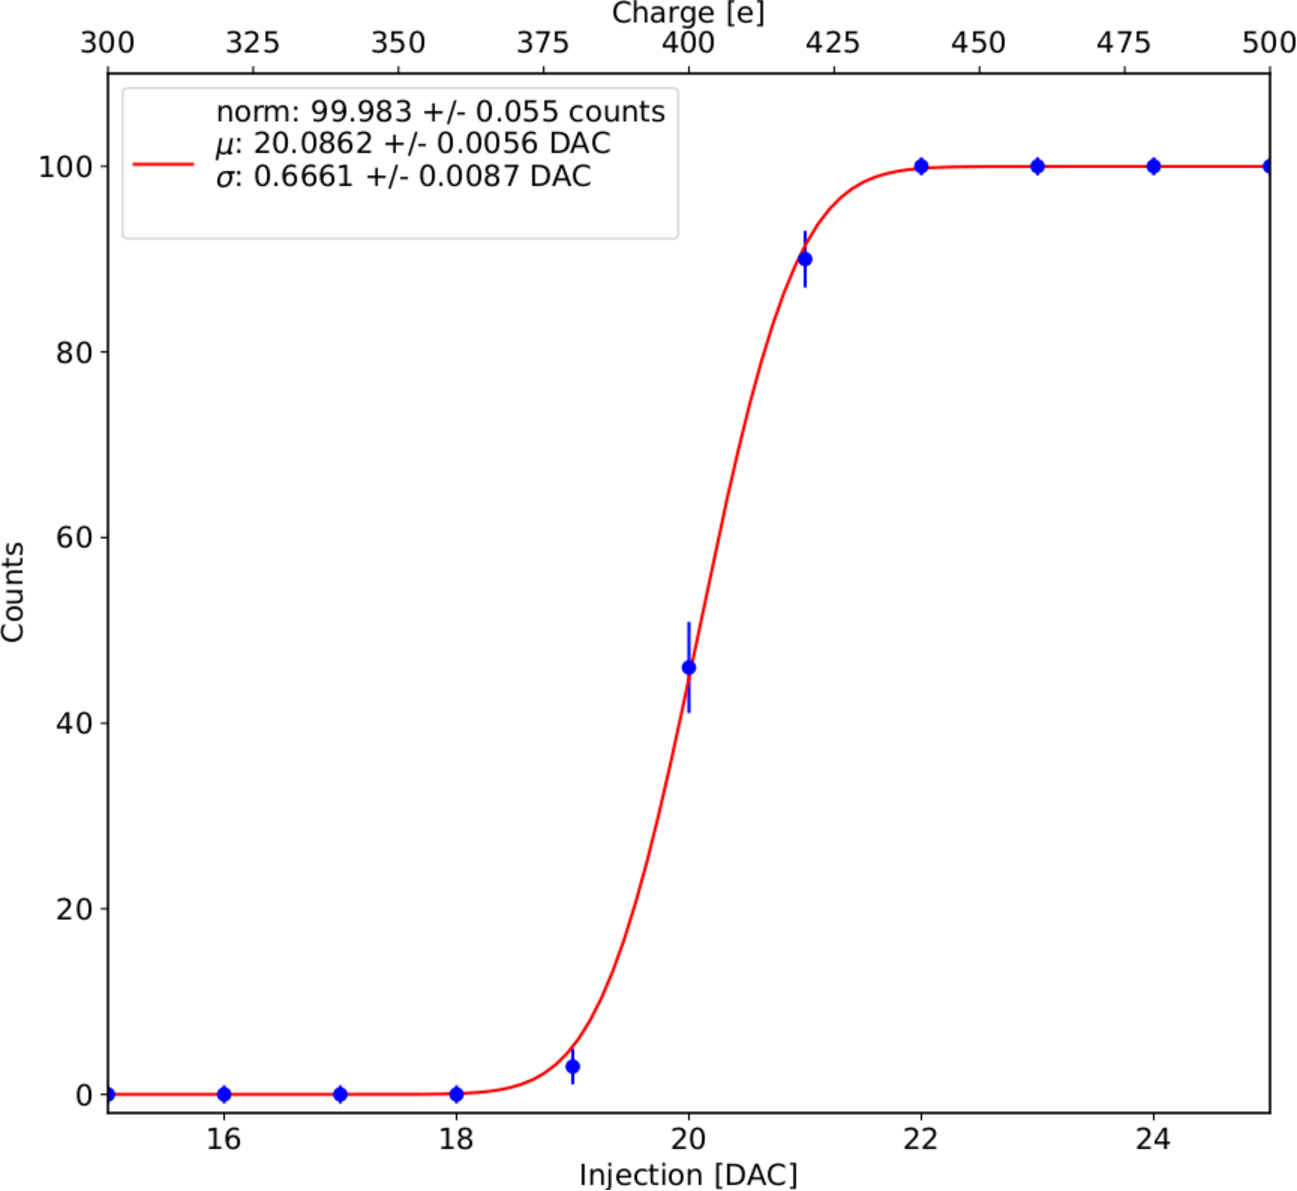
\includegraphics[width=.6\linewidth]{figures/charaterization/scurve.pdf}
            \caption{S-curve for pixel (10, 10) of the PMOS flavor (flavor 1) with IDB fixed at \SI{40}{DAC}. The conversion of charge injected from DAC to electrons has been done assuming a conversion factor of \SI{20}{e-/DAC}. }
            \label{fig:scurve}
        \end{figure}   
        Assuming a gaussian noise, the efficiency of detecting the signal can be described through a modification of the error function:
        \begin{equation}
            f(x, \mu, \sigma) = \frac{1}{2} \; \left(1\,+\,erf\left(\frac{x-\mu}{\sigma \sqrt{2}}\right)\right)
            \label{eq:fit_scurve}
        \end{equation}
        \red{with:} 
        %\begin{equation} 
        %    erf(z) = \[ \int_{0}^{z} \frac{2}{\sqrt{\pi}} e^{-x^2} dx  \]
        %\end{equation} 
        where the threshold and the ENC corresponds to the $\mu$ and $\sigma$.
        Therefore I perform a fit of the counts detected using the function in equation \ref{eq:fit_scurve}. In figure \ref{fig:scurve} there is an example with IDB equal to \SI{40}{DAC} of fit for a pixel belonging to the flavor B, while in table \ref{tab:Flavor_PMOS_reser} and figure \ref{fig:threshold_noise_hist} there are the histograms and the maps of the parameters of the scurve-fit. As expected, the flavor PMOS reset gated (A), thanks to the transistor which change the baseline value, has a lower threshold and noise
        \begin{figure}[h!]
            \centering
            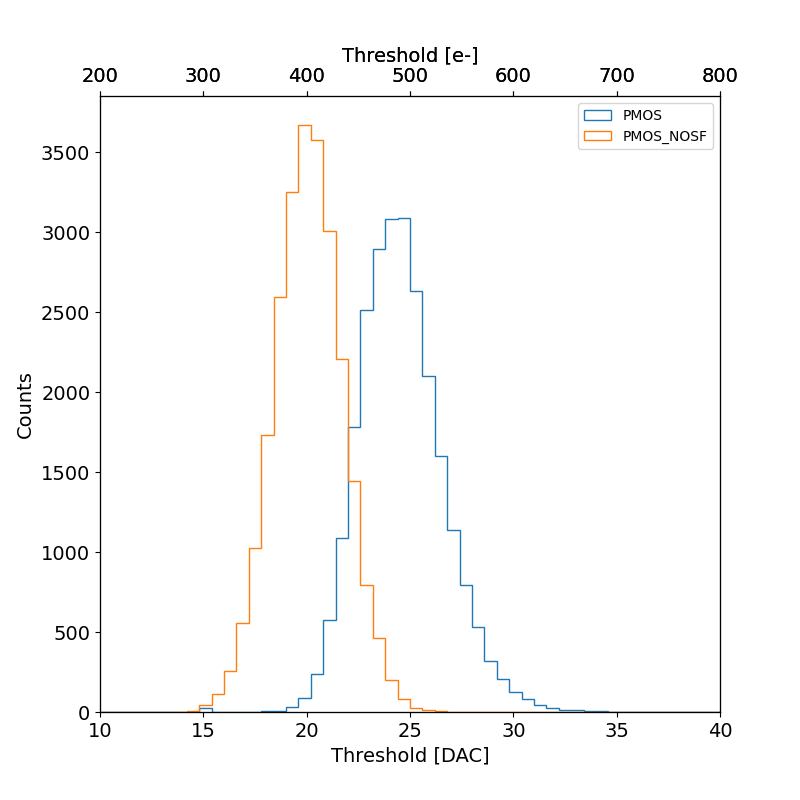
\includegraphics[width=.49\linewidth]{figures/charaterization/threshold_histogram.png}
            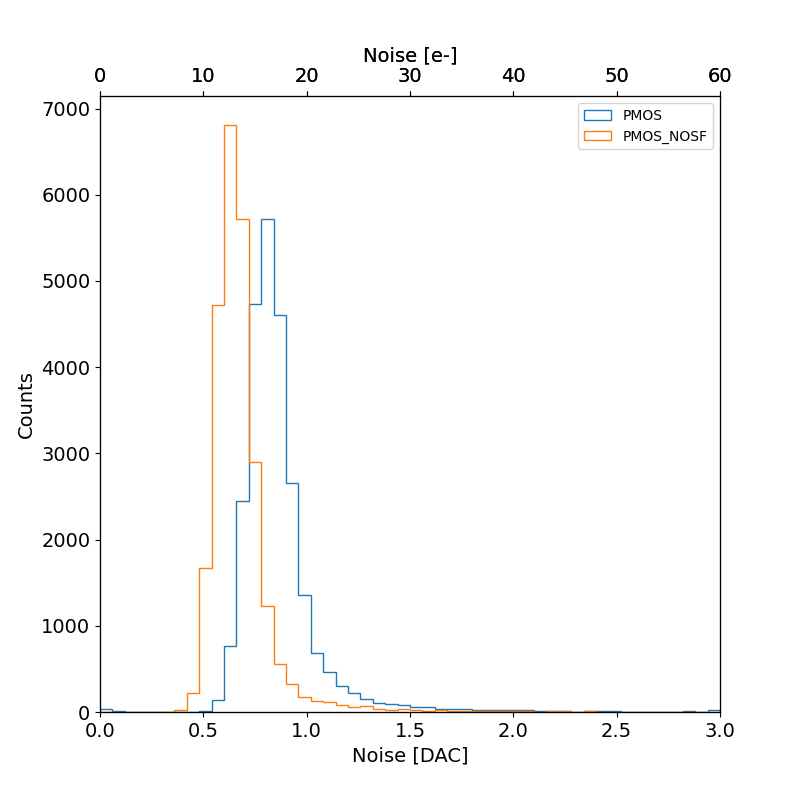
\includegraphics[width=.49\linewidth]{figures/charaterization/noise_histogram.png}\\
            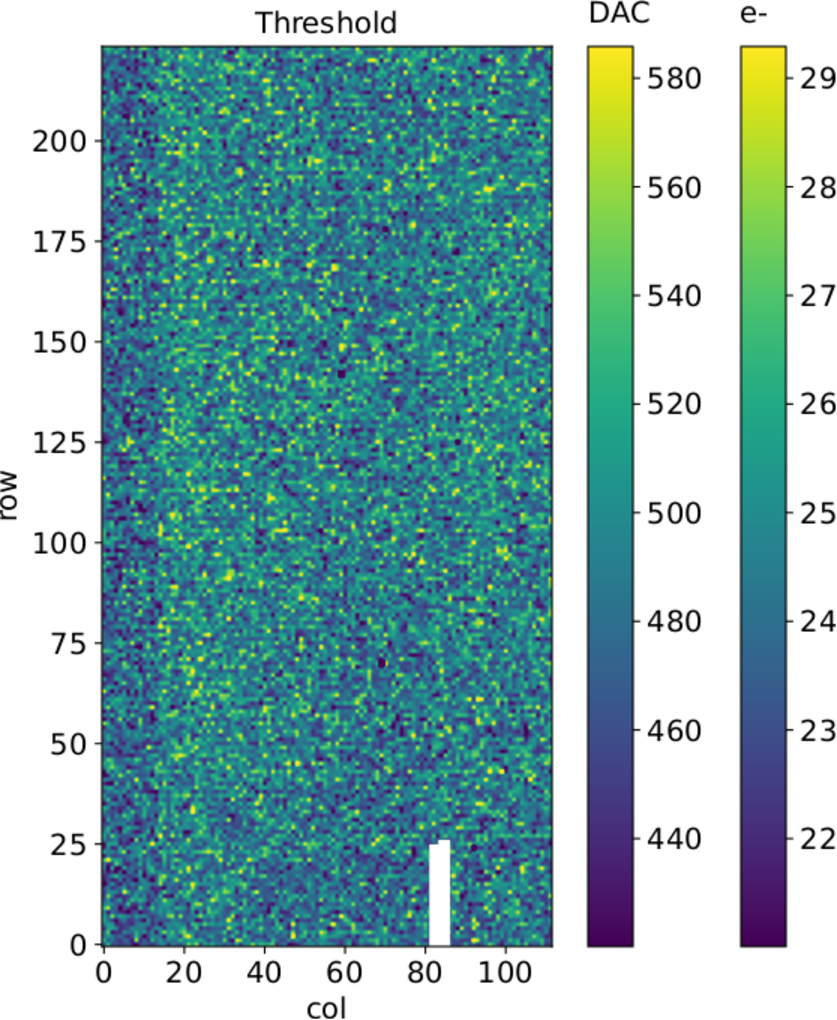
\includegraphics[width=.49\linewidth]{figures/charaterization/threshold_map.pdf}
            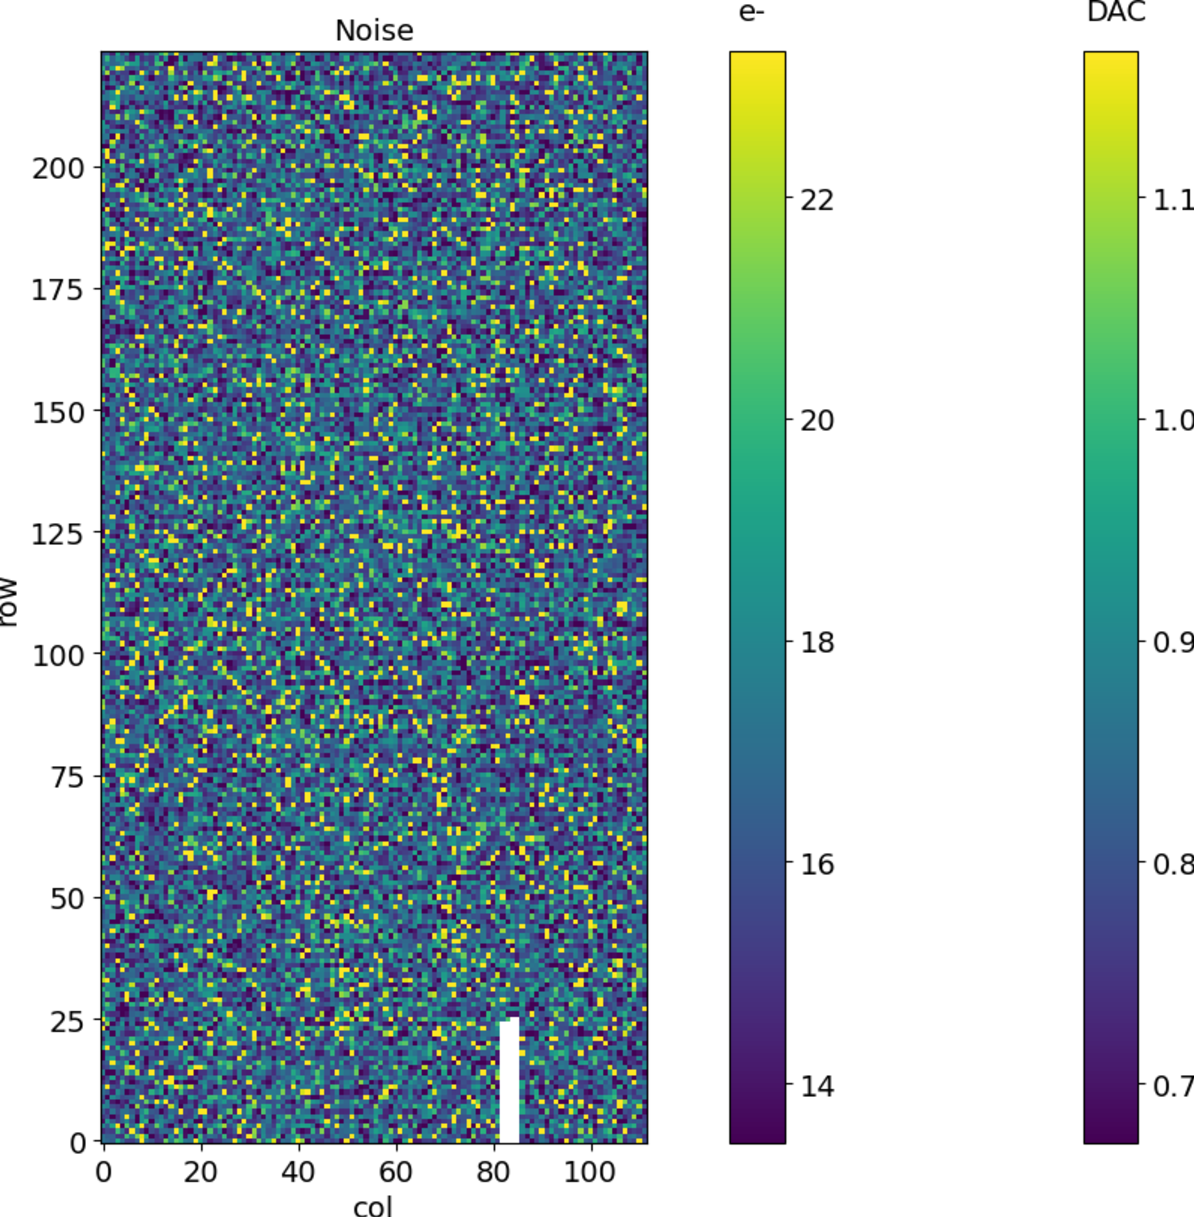
\includegraphics[width=.49\linewidth]{figures/charaterization/noise_map.pdf}            
            \label{fig:threshold_noise_hist}
            \caption{Histograms of the threshold (a) and the noise (b) found fitting the s-curve of \red{all} flavor with IDB fixed at \SI{40}{DAC}. Below there are the maps of the threshold (a) and the noise (b), respectively, found fitting the s-curve with IDB fixed at \SI{40}{DAC} for the PMOS flavor (B). The white pixels have the injection circuit broken.}
        \end{figure}      
        \begin{table}
                \begin{center}
                \begin{tabular}{| c | c | c |}
                \hline
                 & DAC units & electrons \\
                \hline
                \hline
                Threshold        & 24.529 $\pm$ 0.049 & 511.0 $\pm$ 1.0 \\
                Threshold dispersion & 1.848 $\pm$ 0.033 & 36.96$\pm$0.66\\
                Noise            & 0.8222 $\pm$ 0.0043 & 16.444$\pm$0.086 \\
                Noise dispersion & 0.0975 $\pm$ 0.0030 & 1.95$\pm$0.06\\
                \hline
                \end{tabular}
                \caption{Flavor PMOS, IDB fixed at \SI{40}{DAC}}
                \label{tab:Flavor_PMOS_reser}
                \end{center}
        \end{table}        
    
        %Furthermore the two portion of the chip, with FDPW and with RDPW, have been analyzed separately, because a small difference in the sensor input capacitance was expected: in fact, the deep p-well removal in the RDPW causes a small reduction of the depletion region around the collection electrode, which results in an increase of the sensor capacitance C.
        %\red{Then  , the charge to voltage conversion gain at the front-end input (Q /C ) is lower and as a result, for the same input charge a lower voltage amplitude is induced at the front-end input. }
    
    
        Small threshold variations has been observed in the first biasing section (columns from 0 to 14) with IDB=\SI{40}{DAC}; the same structure appears more evident at other different IDBs,as for example \SI{100}{DAC}
        \red{Plot of the average threshold per column al variare di IDB.} 
        The systematic threshold variation across the biasing group has not a known motivation, but one could certainly be the transistor mismatch of the biasing DAC registers IDB and ICASN, which both adjust the effective threshold (I recall that ICASN regulate the baseline, and in this measurements it was set to the minimin possible value).

        %GUARDA A PAGINA 127 DELLA TESI PER GLI ULTIMI DUE FLAVOR

        To verified the trend of the threshold as a function of the front end parameter IDB and find its dynamic range, I have permormed different scans changing the IDB: I have injected the whole matrix and found the means and the standard deviation of the distributions. The results are shown in figure \ref{fig:threshold_vs_IDB}: the blue points are the mean threhsold found whithin the matrix, while in green is shown the width of the threshold distribution, aka the threshold dispersion. 
        While the threshold increases, the ENC decreases of $\sim$\SI{4}{e-},which is $\sim$1/3 of the noise at IDB=\SI{40}{DAC}. 
        \begin{figure}[h!]
            \centering
            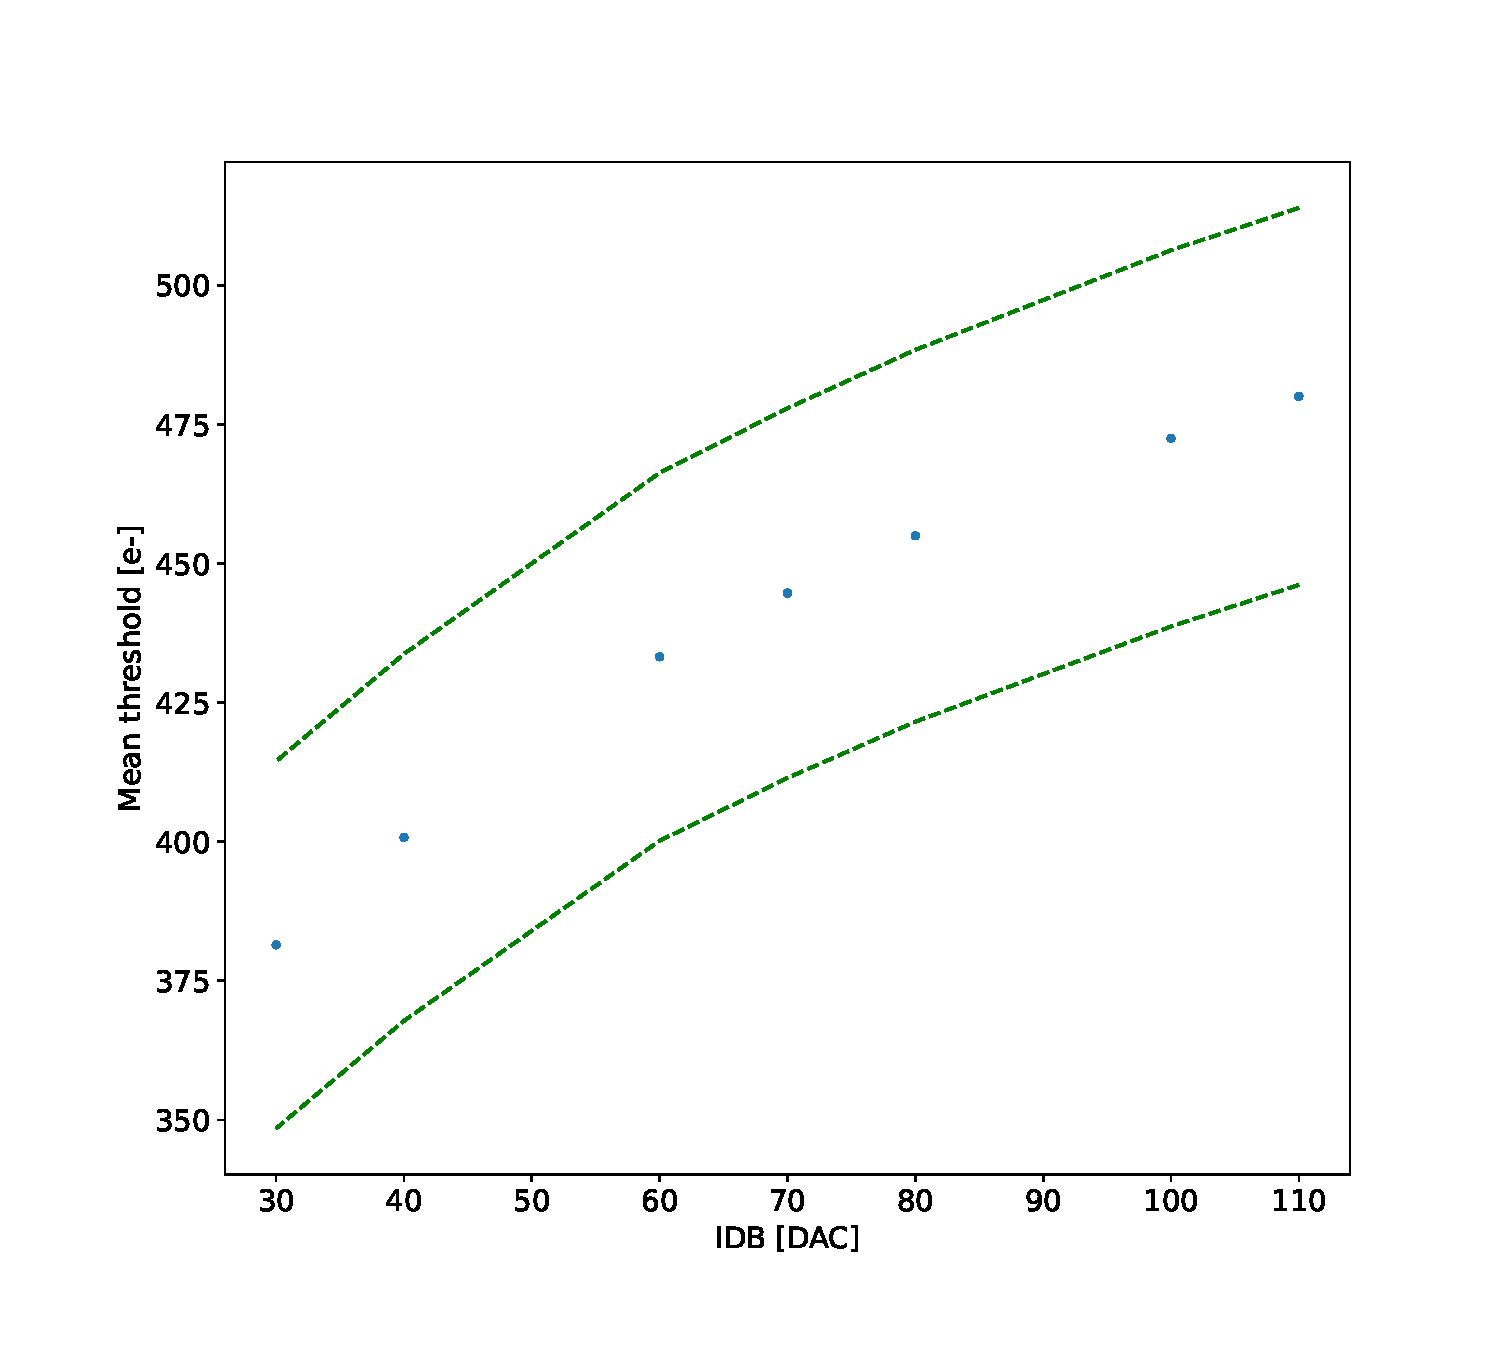
\includegraphics[width=.70\linewidth]{figures/charaterization/thr_vs_IDB.pdf}
            \caption{Flavor PMOS (B) with Psub-Pwell biased at -\SI{6}{V}.Threshold measured in electrons vs the register which sets the threshold, IDB.  }
            \label{fig:threshold_vs_IDB}
        \end{figure}            

        Then, to evaluete the operation and the occupancy of the chip at different threshold I have made long acquisitions of noise at different IDB and check how the number of pixel masked changes with the threshold. The masking algorithm I have used search for pixels with rate $>$\SI{10}{Hz} and mask them. With such algorithm, in our standard condition, IDB=\SI{40}{DAC}, a very low noise hit rate is intentionally achieved masking only \red{dozen of pixels?} of the whole flavor, and other \red{quanti} are unintentionally masked. 

    \subsection{Linearity of the ToT}    
        %python3 -i acquisition_Fe55/fit_tot_single_pixel.py -f acquisition_Fe55/source_PMOSS/ per fare il fit    
        %python3 -i acquisition_Fe55/plot_tot_single_pixel.py -f acquisition_Fe55/source_PMOSS/ -fl 'gauss_line' per fare il plot di single pixel
        I have already said in chapter \ref{chap:Monopix1} that TJ-Monopix1 returns an output signal proportional to the charge released by a particle in the epitaxial layer, which is the Time over Threshold; the ToT is saved as a 6-bit variable and then has a dynamic range equal to 0-64, which corresponds to \SIrange{0}{1.6}{\us} assuming a clock frequency of \SI{40}{MHz}.
        When a pulse is longer than \SI{1.6}{\us} the counter rolls back to zero and there is no way to distinguish that charge from a lower one with the same ToT: that is the rollover of the ToT (\ref{fig:ToT_vs_charge}(a)).   

        In order to associate the ToT (in range 0-64) to the charge, a calibration of the signal is necessary. Assuming the linearity between ToT and the charge, Q can be found: 
        \begin{equation}
            Q\, [DAC] = \frac{(ToT\,[au]\, -\, q\,[au])}{m\, [au/DAC]} 
        \end{equation}
        where m and q are the fitted parameters of the calibration.
        It is important to keep in mind that the main application target of TJ-Monopix1 is in the inner tracker detector of HEP experiments, then the main feature is the efficiency, then a rough calibration of the signal to charge is fine. The ToT information can be used both to better reconstruct the charge deposition in cluster in order to improve the track resolution, and for particle identification, especially for low momentum particles which do not reach the proper detectors.
                        
        The study of the output signal is made possibile via the injection: since the pulses are triangular, the ToT is expected to be almost linear depending on the injection charge value.
        To verify this statement and study the deviations from linearity I've fit the ToT versus the charge injected for all pixel within the matrix.
        In figure \ref{fig:ToT_vs_charge}(b) there is an example of fit for a pixel belonging to the flavor B, while in figure \ref{fig:ToT_histograms_all_fl} there are the histograms and the maps of the parameters of the line-fit for all flavors with IDB fixed at \SI{40}{DAC}. Here again a difference between biasing section appears: since the slope of the ToT is related with the gain of the preamplifier (increasing the gain also increases the ToT), the mismatch is probably due to the transistor contributing to the amplification stage.

        Before performing the fit I have calculated the mean value of the ToT of the pulses recorded for each pulse amplitude and I used the mean ToT as value for the fit. 
        The aim of the calibration obviously is finding a relation only in the range 0-64 without taking into account the rolling over hits: therefore, to prevent the rollover data from reducing the mean ToT introducing a bias in the mean value, I cut and I did not consider them. 
        If a signal bigger than the \SI{1.6}{\us} is expected in the usage of the detector, the threshold must be raised or the gain reduced, making the expected output signal in range 0-64. 
        In figure \ref{fig:ToT_vs_charge} (b) are shown both the fits with a line (red) and with a second order polynomial (green): at the bounds of the ToT range values deviate from the line model. Since the deviation is low than 1\% and it only interest the region near the 0 and the 64, in first approximation it is negligible. 
        
        \begin{figure}[h!]
            \centering
            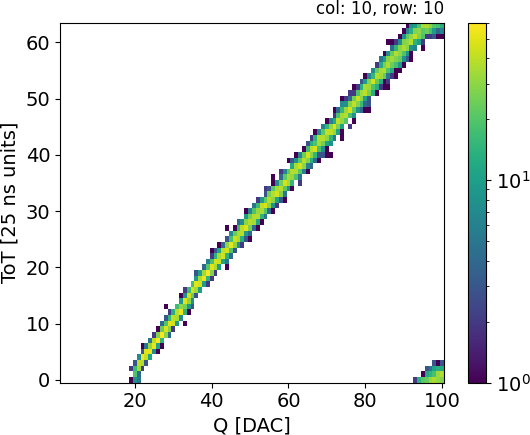
\includegraphics[width=.49\linewidth]{figures/charaterization/ToT_rollover.png}            
            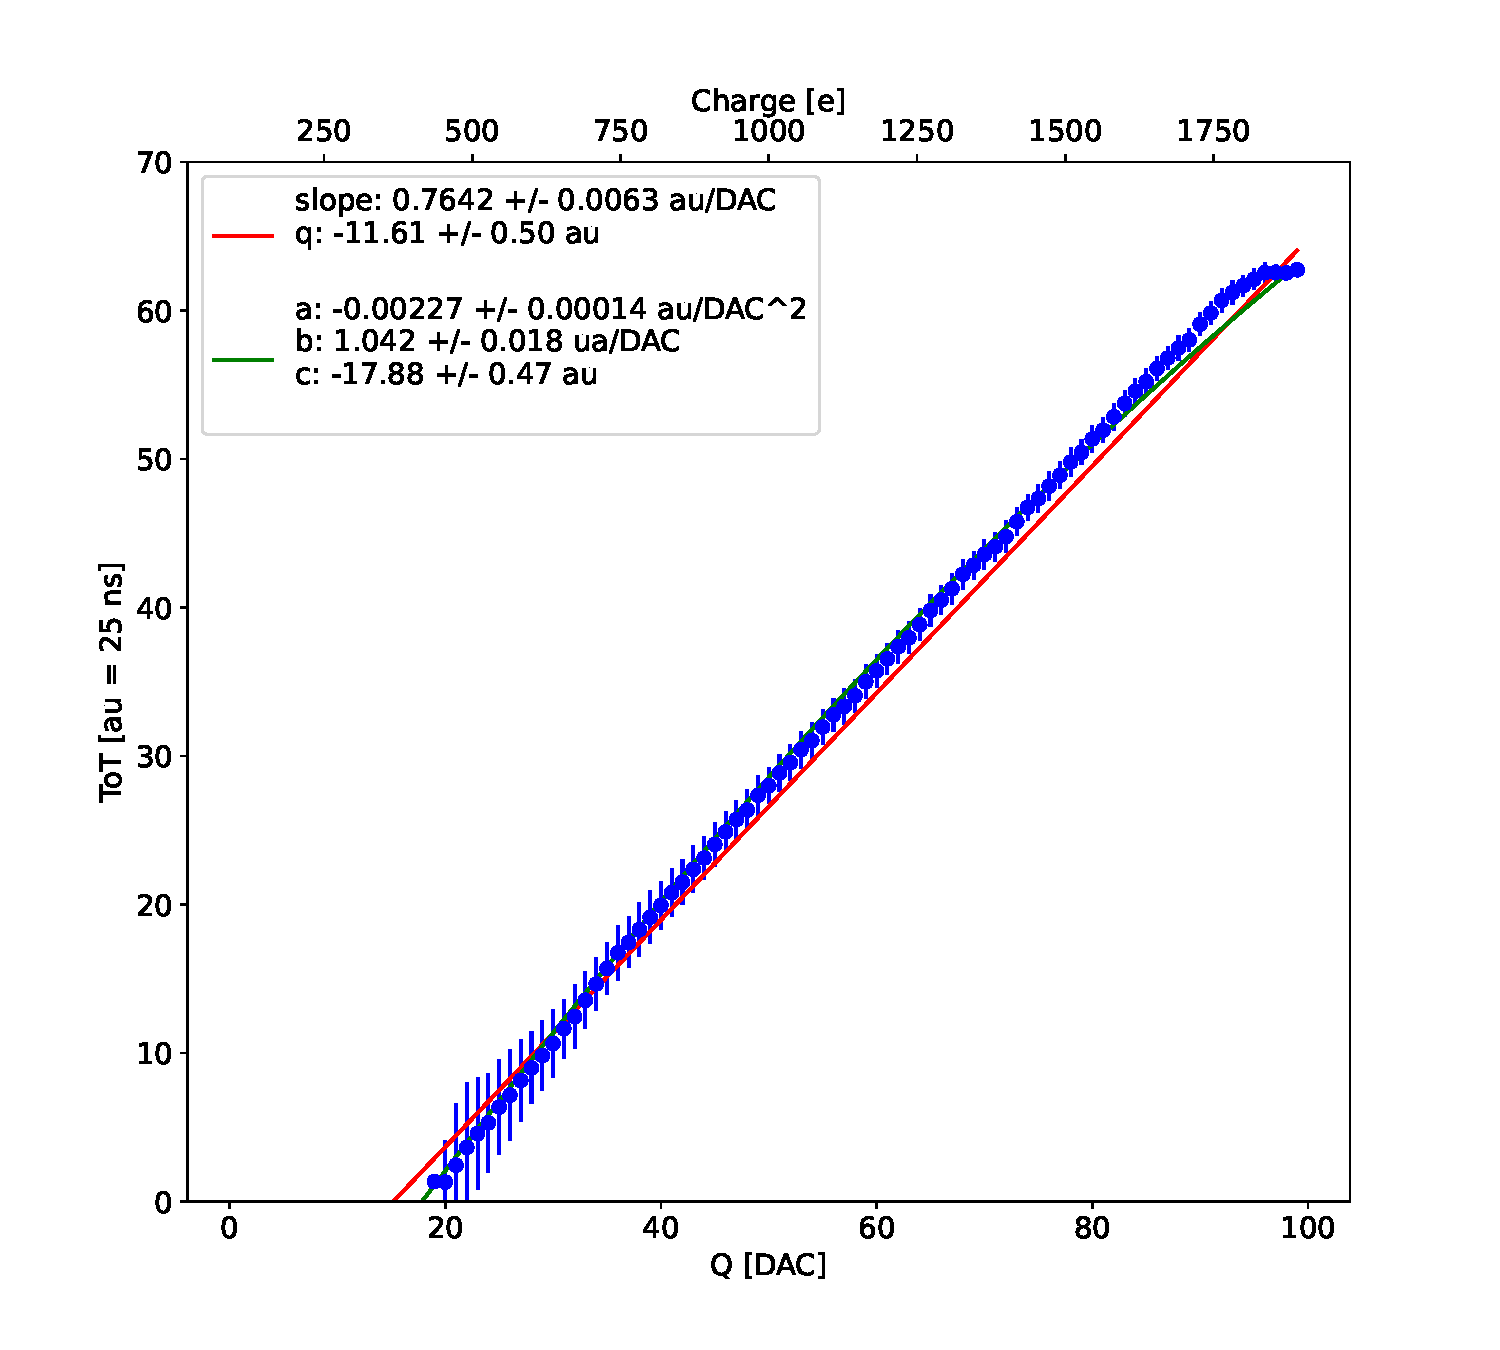
\includegraphics[width=.49\linewidth]{figures/charaterization/ToT_injection.pdf}
            \label{fig:ToT_vs_charge}
            \caption{The figures refer to pixel (10,10) of the PMOS-reset flavor (1) with IDB fixed at \SI{40}{DAC} for the PMOS flavor (B).
            (a) Histogram of the injection pulses: the ToT is in range 0-64 since it is represented by 6 bit, so when achieving the 64 it rolls over back to the zero. (b) Mean ToT vs the the charge: the mean has been calculated cutted the rolling hits. }
        \end{figure}    

        \begin{figure}[h!]
            \centering
            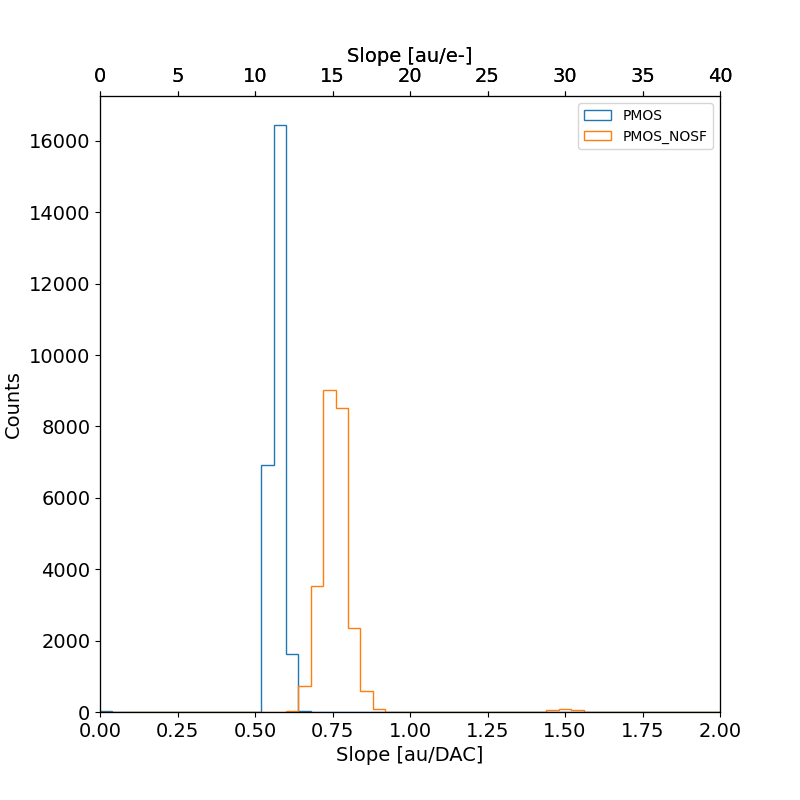
\includegraphics[width=.49\linewidth]{figures/charaterization/slope_histogram.png}
            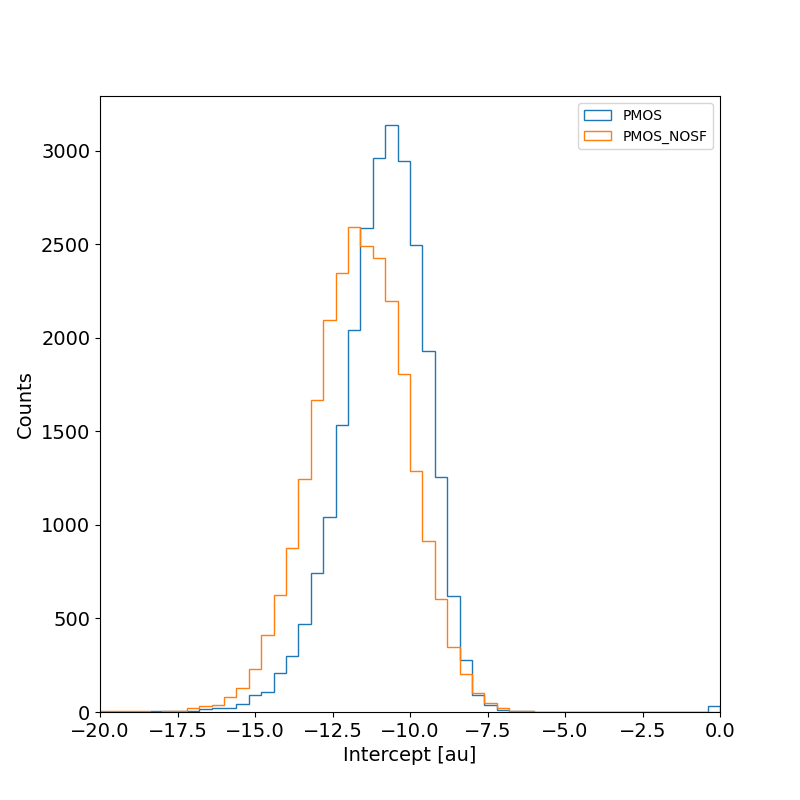
\includegraphics[width=.49\linewidth]{figures/charaterization/intercept_histogram.png}\\
            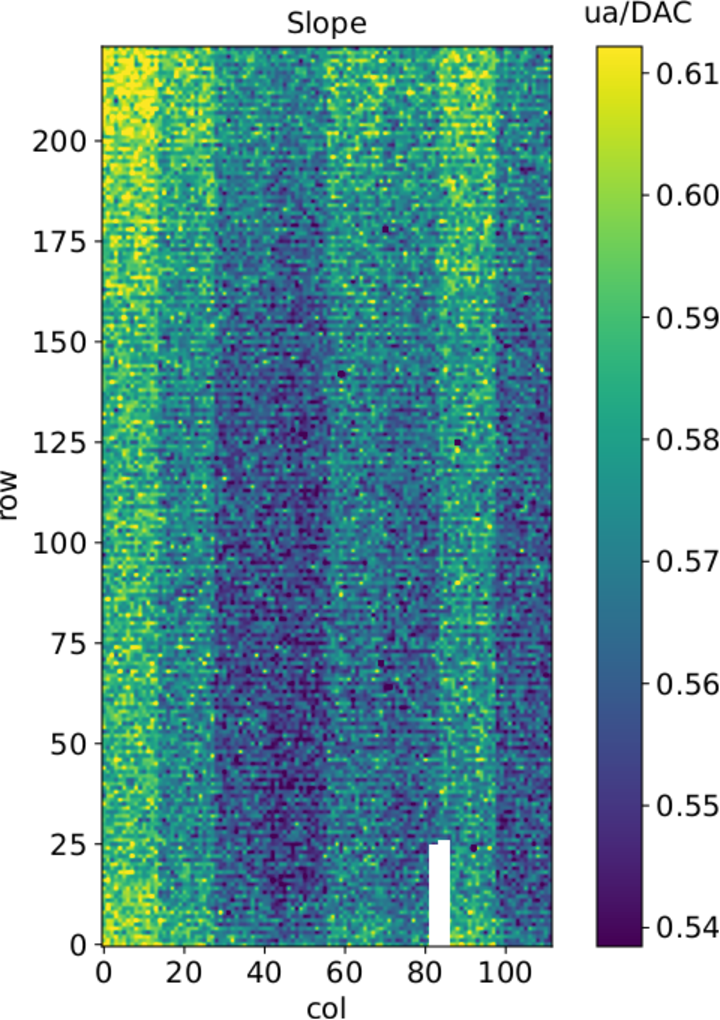
\includegraphics[width=.49\linewidth]{figures/charaterization/slope_map.pdf}
            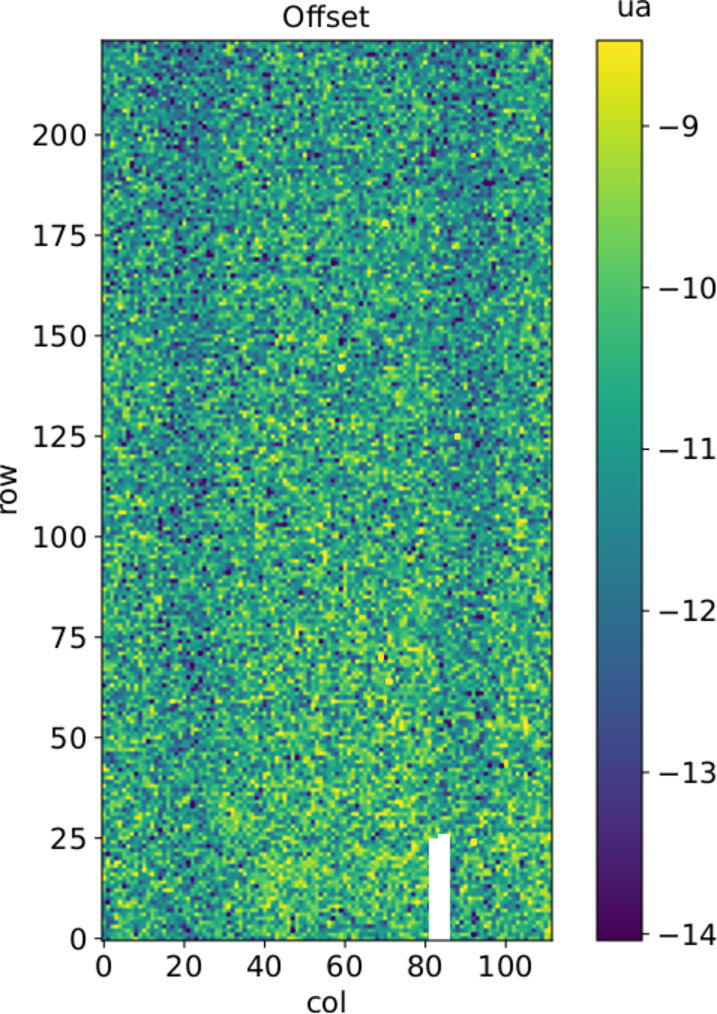
\includegraphics[width=.49\linewidth]{figures/charaterization/offset_map.pdf}
            \caption{Histograms of the calibration parameters, slope (a) and offset (b), found fitting the ToT with a line, for \red{all} flavor and with IDB fixed at \SI{40}{DAC}. Maps of the calibration parameters, slope (a) and offset (b), found fitting the ToT with a line, with IDB fixed at \SI{40}{DAC}}
            \label{fig:ToT_histograms_all_fl}
        \end{figure} 


        \begin{table}
            \begin{center}
            \begin{tabular}{| c |  c | c | c |c |}
            \hline
            & PMOS 0 & PMOS 1 & PMOS 2 & HV \\
            \hline
            \hline
            Slope [au/DAC] & 0 .75566 $\pm$ 0.00149 & 0.57145 $\pm$ 0.00025 \\
            Slope dispersion [au/DAC] & 0.03841 $\pm$ 0.00037 & 0.01685 $\pm$ 0.00016\\
            Intercept [au] & -11.6070 $\pm$ 0.0089 & -10.824 $\pm$ 0.019 \\
            Intercept dispersion [au] & 1.5176 $\pm$ 0.0063 & 1.225 $\pm$ 0.013\\
            \hline
            \end{tabular}
            \caption{Mean calibration parameters for \red{all} flavor and their dispersion on the matrix. }
            \label{tab:calibration_param}
            \end{center}
        \end{table}        

    \subsection{Calibration of the ToT}
        \begin{figure}[h!]
            \centering
            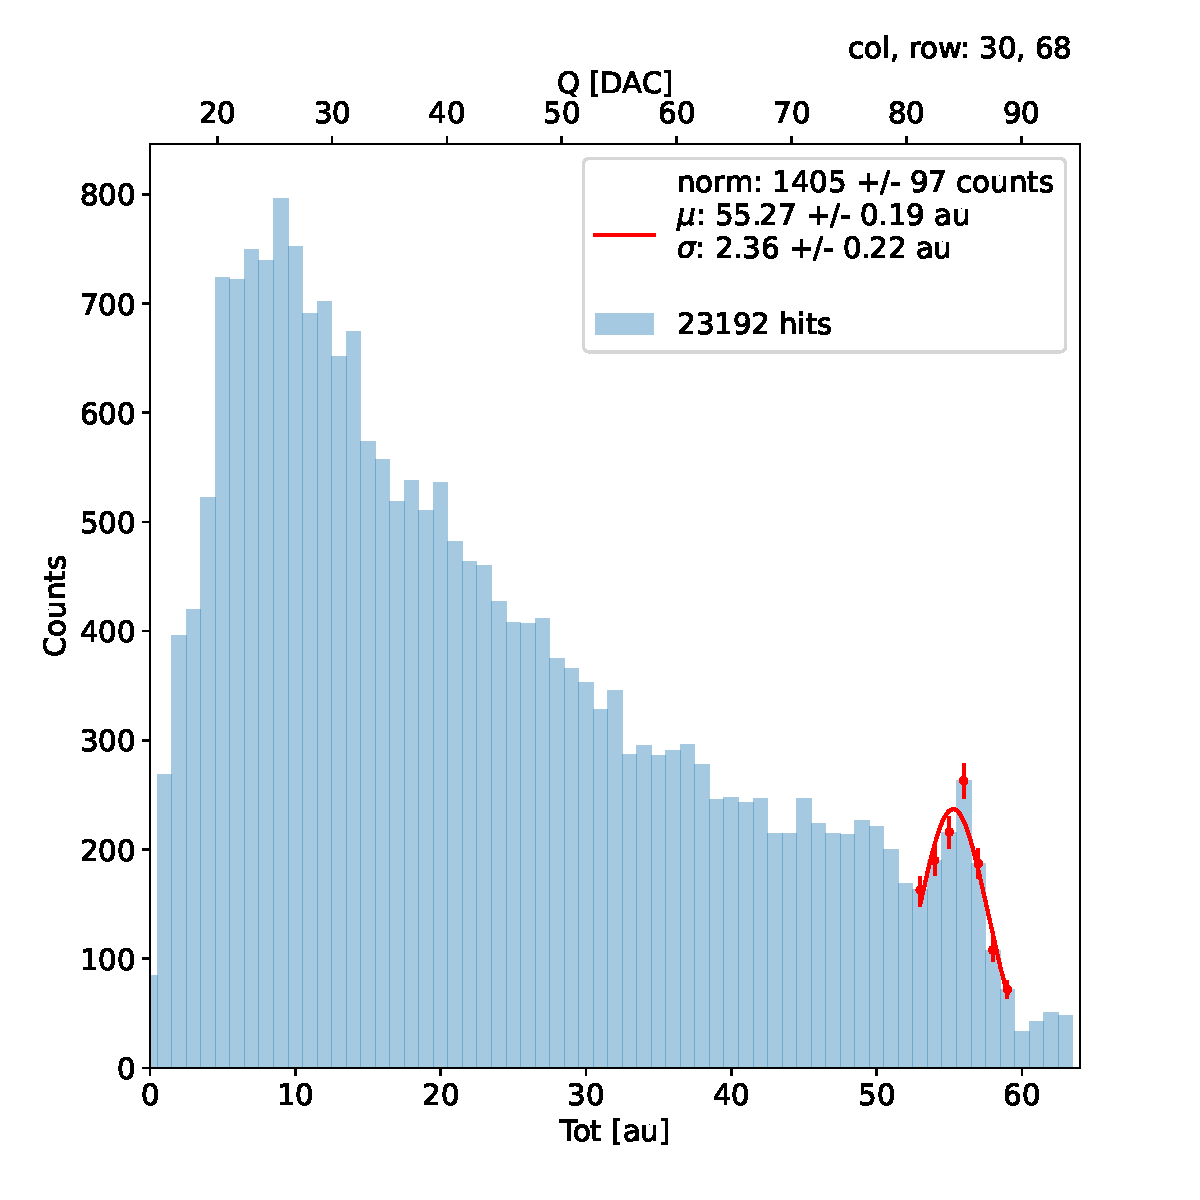
\includegraphics[width=.49\linewidth]{figures/charaterization/fit_gauss_r69.pdf}
            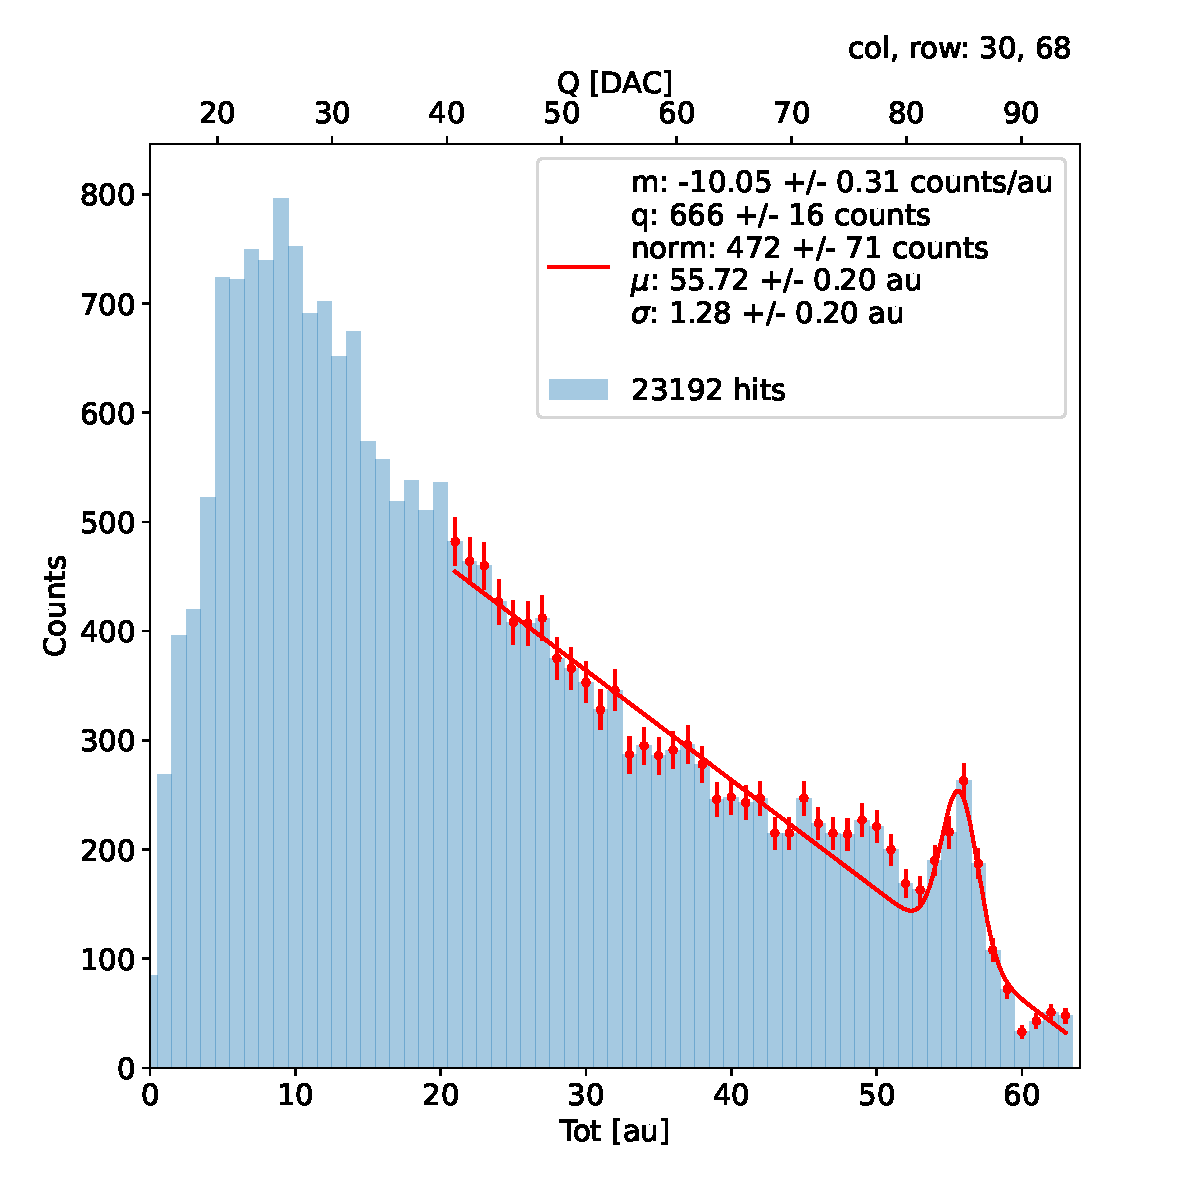
\includegraphics[width=.49\linewidth]{figures/charaterization/fit_line_gauss_r69.pdf}\\
            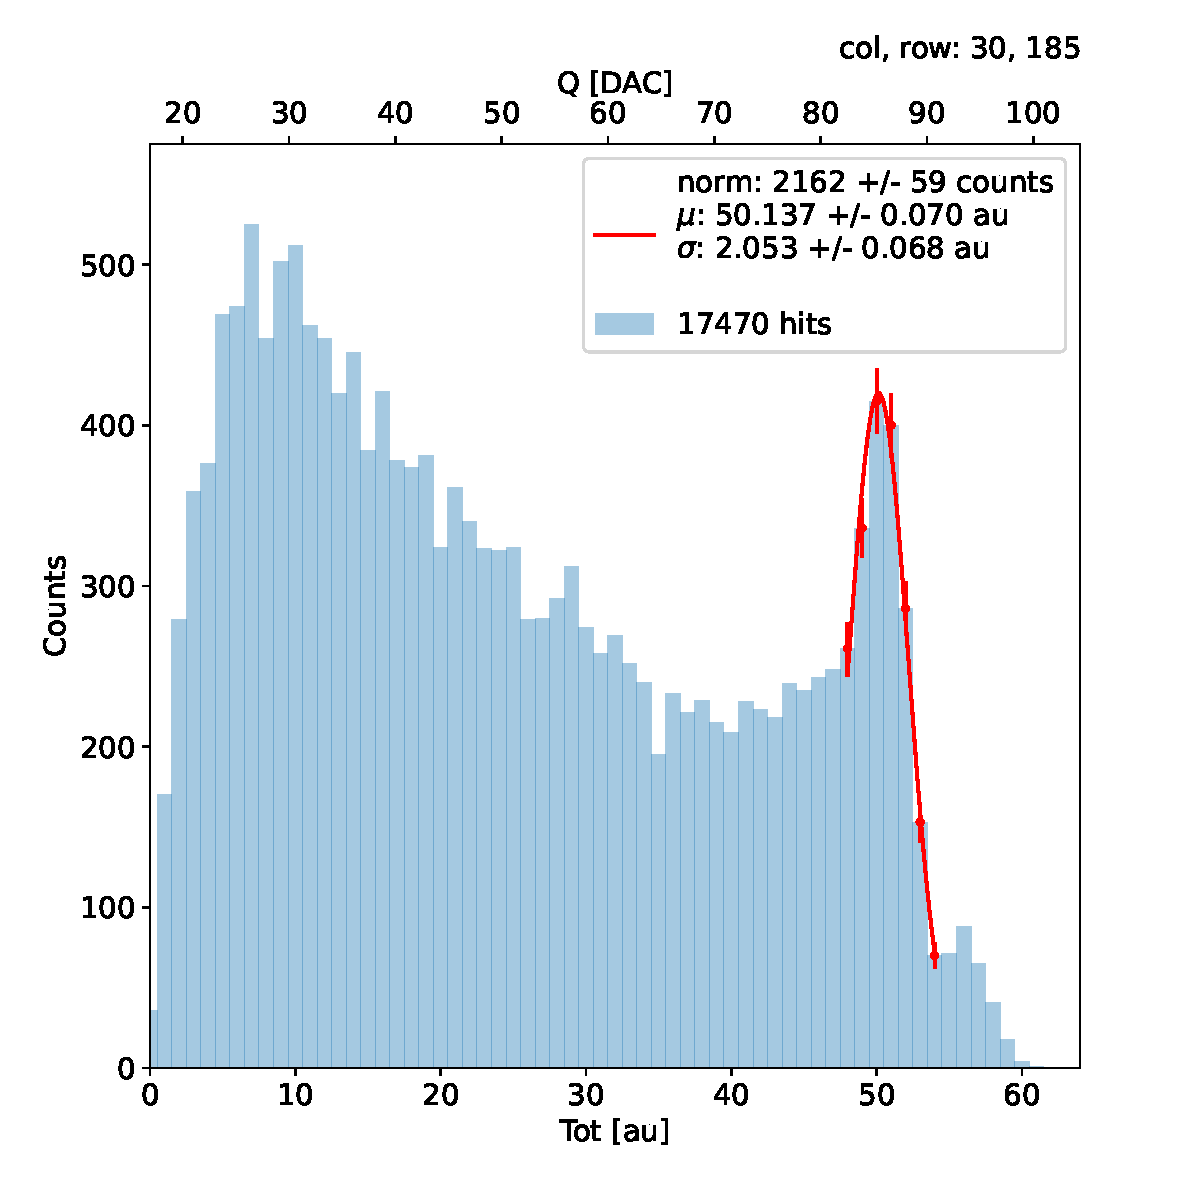
\includegraphics[width=.49\linewidth]{figures/charaterization/fit_gauss_r185.pdf}
            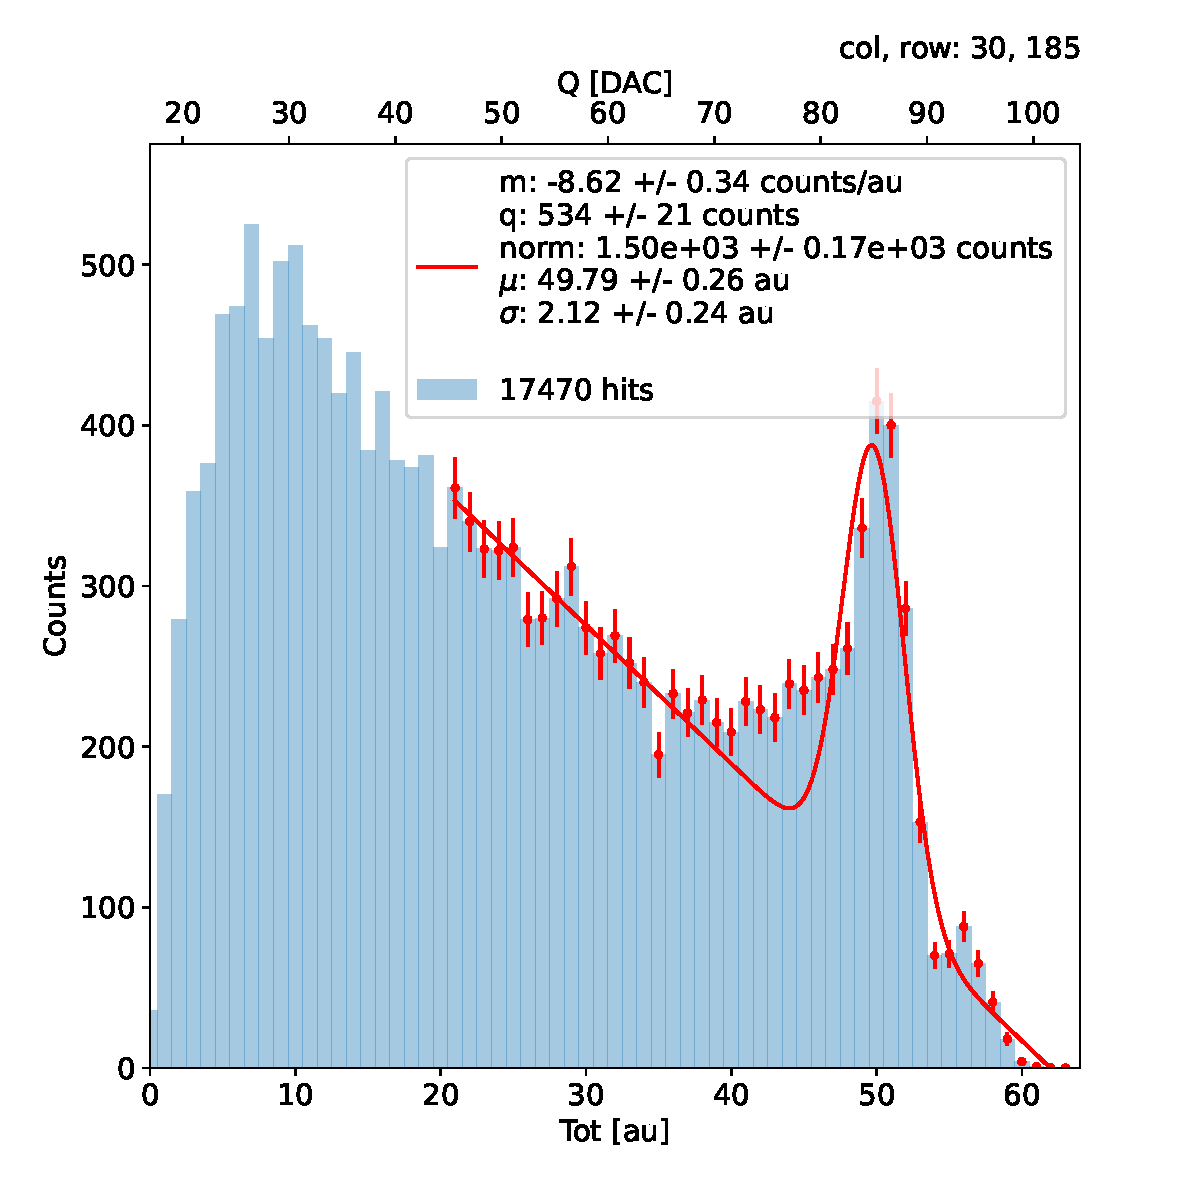
\includegraphics[width=.49\linewidth]{figures/charaterization/fit_line_gauss_r185.pdf}
            \caption{due pixel per far vedere la differenza tra i fit. Sottolinea che in rosso ci sono i bin fittati. La doppia scala utilizza le info trovate nel paragrafo precedente per il dato pixel in questione. Per avere una corrispondenza grezza in elettroni basta moltiplicare per 20 e- dac. }
        \end{figure}  
        %python3 -i acquisition_Fe55/fit_tot_single_pixel.py -f acquisition_Fe55/source_PMOSS/Fe_acquisitions_6V/ per fare i fit. Attenzione che prende i file degli istogrammi npz già
        Considering that the charge injected in the FE goes to fill capacitor which is different from pixel to pixel, the true charge injected does not correspond to what expected assuming C equal to \SI{230}{aF}, the nominal value. 
        Accordingly to that, a verification of the value provided and an absolute calibration of this capacity and of the conversion factor F is needed to have a correspondence of the signal in electrons; assuming C \SI{230}{aF}, F is expected to be \SI{20}{e-/DAC}, and is defined as:
        \begin{equation}
            F\, [e-/DAC] = \frac{1616\,e-}{Q\,[DAC]}
        \end{equation}

        For this pourpose a Fe55 radioactive source has been employed; the Fe55 is en extremely important radionuclide in the calibration of X-ray spectrometers, proportional counter and scintillator detector since it emits two two X-photons during the electron capture decay: the first one (K$_\alpha$) at \SI{5.9}{keV} and the second one (K$_\beta$) at \SI{6.5}{keV}.
        The K$_\alpha$ photon, which does photoelectric effect in the silicum, has an absorption length $\lambda$=\SIrange{7}{8}{\um}, and the probability of being assorbed in the \SI{25}{\um} thick epitaxyal layer is $\sim$0.95\.
        The electron emitted has an energy equal to the photon one, so recalling that the mean energy needed to produce a couple electron-vacuum is \SI{3.65}{eV}, the signal produced by the Fe55 source is expected to be \SI{1616}{e-}.
        In figures \ref{fig:fit_r185} and \ref{fig:fit_r69} are shown two histograms of the ToT spectrum of the Fe55 source for two different pixels. The peak corresponds to the events with completely absorption of the charge produced in the depleted region, while the long tail on the left to all the events with partial absorption due to charge sharing among neighbors pixels. In order to reduce the charge sharing, the pixel dimension in TJ-Monopix2 has been reduced down to 30$\times$\SI{30}{\um\squared}. 
        The events on the right side of the peak, instead, corresponds to the K$_{\beta}$ photons. 
        Looking at the histograms for pixel (30, 185) and (30,69) a significant difference in the peak to tail ratio leaps out. 
        This difference in the efficiency of detecting the signal can be related with the position of the pixel in the matrix: in particular pixels in the upper part of the matrix (rows 112-224) have a more prominent peak, while in pixels in the lower part (rows 0-111) there is a higher partial absorption. 
        I recall now that there is a slighly difference in the structure of the low dose-epi layer (\ref{chap:}) among the rows in the matrix, in particular pixels in rows 112-224 are supposed to have a higher efficiency in the pixel corner. 
        
        For the calibration I have need to establish the peak position; to do that I perform a fit of the ToT histogram of each pixels. As fit functions I test both the solutions below:  
        \begin{equation}
            f(x, N, \mu, \sigma) = \frac{N}{\sigma \sqrt{2\pi}} e^{-\frac{1}{2}(\frac{(x-\mu)}{\sigma})^2}
            \label{eq:gauss}
        \end{equation} 

        \begin{equation}
            f(x, m, q, N, \mu, \sigma) = m\,x + q + \frac{N}{\sigma \sqrt{2\pi}} e^{-\frac{1}{2}(\frac{(x-\mu)}{\sigma})^2}
            \label{eq:gauss_line}
        \end{equation}          
        \begin{figure}[h!]
            \centering
            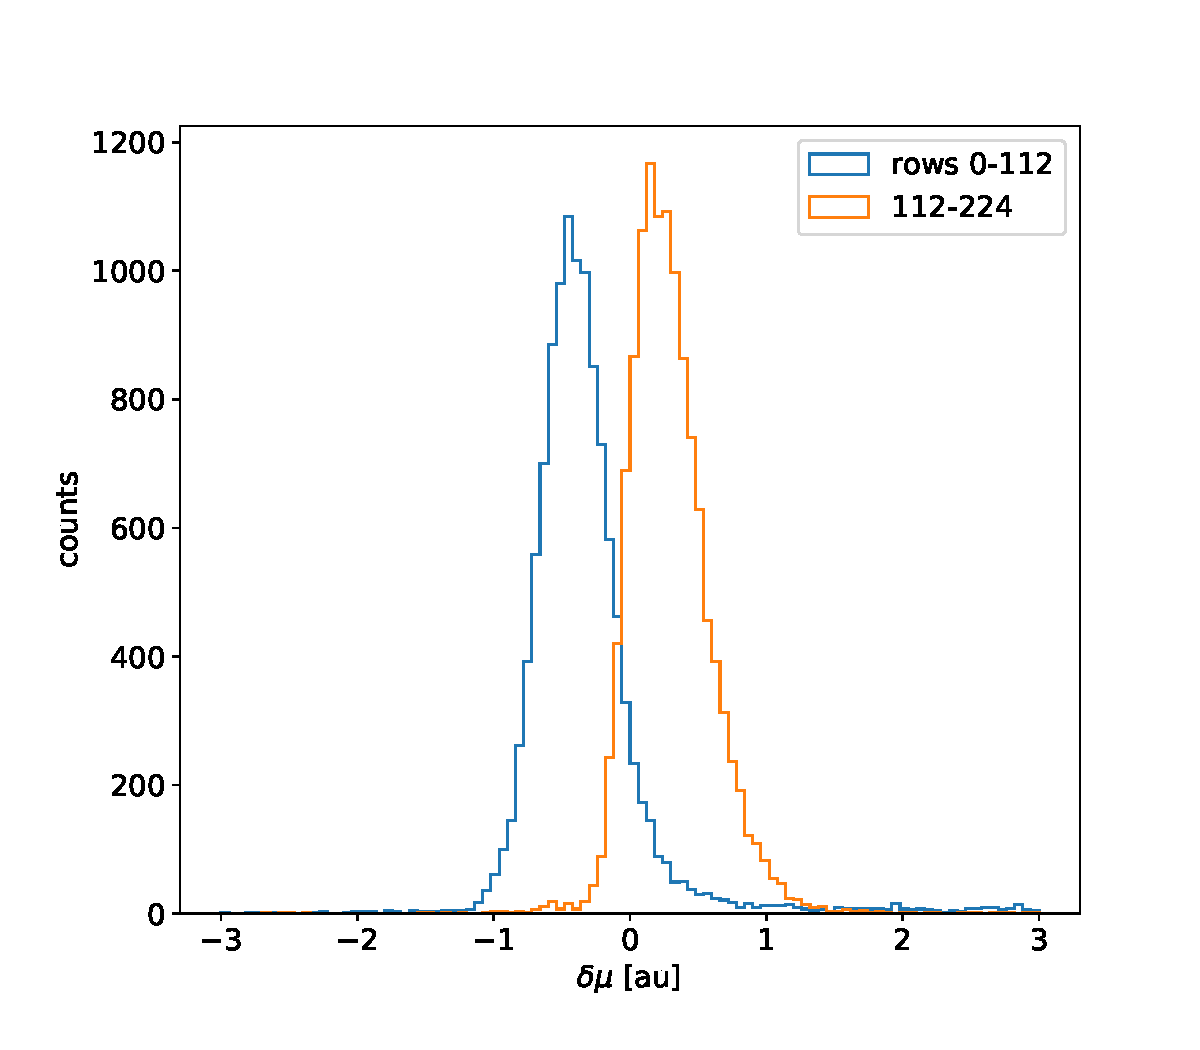
\includegraphics[width=.49\linewidth]{figures/charaterization/deltam_Fe.pdf}
            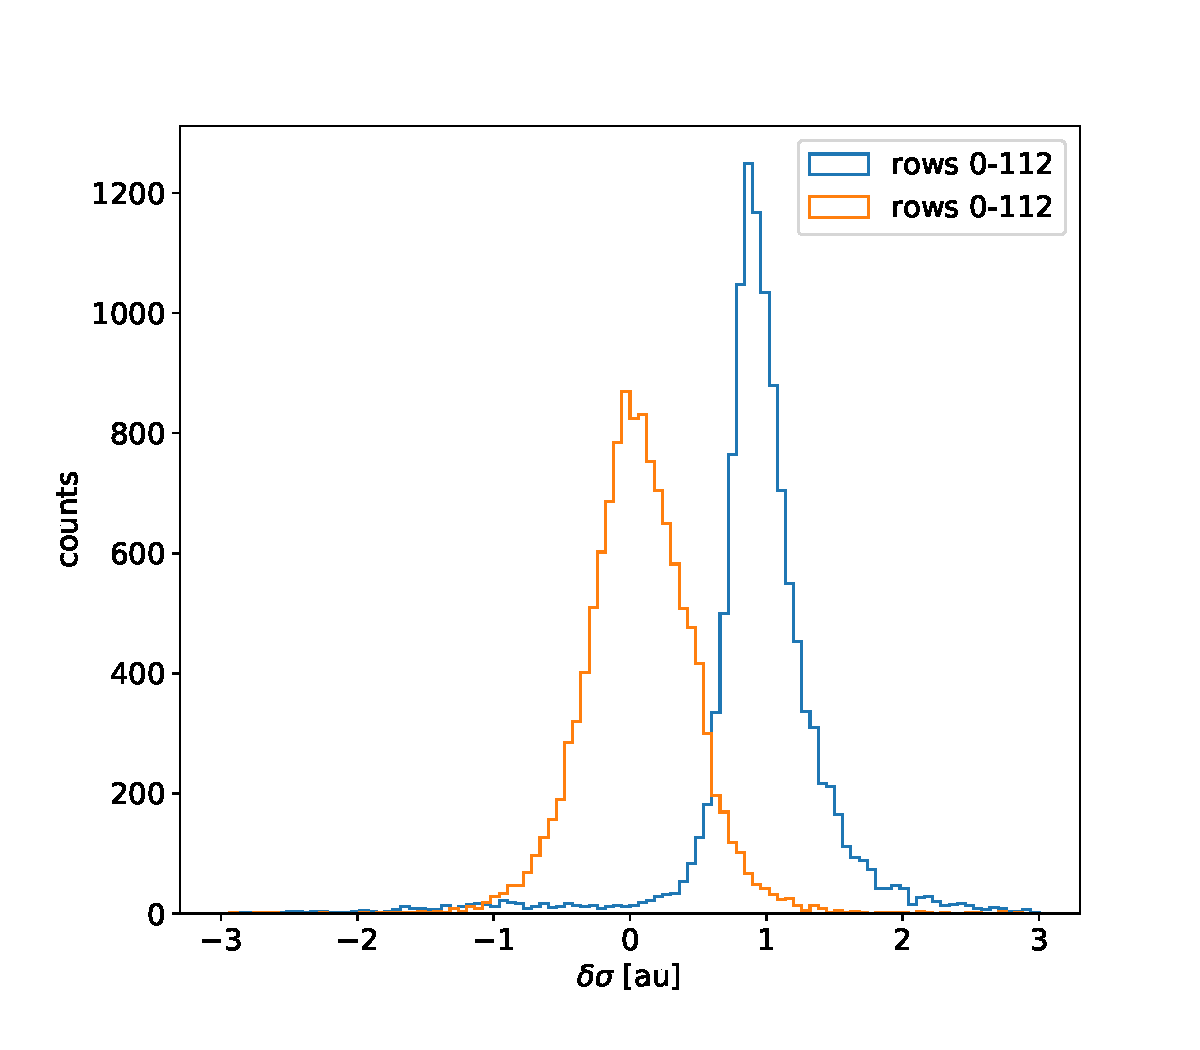
\includegraphics[width=.49\linewidth]{figures/charaterization/deltas_Fe.pdf}
            \caption{Here there are shown the defference between the parameters $\mu$ and $\sigma$ fitted with only a gaussian and with a gaussia plus a line. When $\mu<$0 the fit function \ref{eq:gauss} has given a worst peak (shifted on the left); when $\sigma<0$, \ref{eq:gauss_line} has given a worst peak width (larger sigma)}
            \label{fig:delta_fit}
        \end{figure}           
        \red{Nel primo caso ho fittato pochi pixel attorno a picco: il range è stato determinato .. controlla. 
        Nel secondo caso invece il range è..  Controlla sullo script  }  
        Even if the difference in the peak position between the two cases is not really relevant (\ref{fig:delta_fit}) being of the order of 0.8-1.5 \%,  it still introduces a systematic effect moving the peak on the left beacuse of the contribution of the tail. 
        Indeed, we know that the sharp edge on the right corresponds to the complete absorption of the photon, so excluding the little bump on the right, the more the fitted parameter is on the right, the better the fit is. Moreover, there is also systematic effect on the peak width, infact the worst fit also gives an overestimation of the peak width.  
        Even looking at the $\chi^2$, the fit function \ref{eq:gauss} seems so be the better choise, except for a sample of pixels on the lower part of the matrix, the one with lower efficiency.

        \red{Mappa del ferro da cui, come descritto enll'equazione si ricava la capacity.        
        La struttura a bande della capacità ha origine nel plot... e quindi nella calibrazione. 
        Andando a vedere gli istogrammi di queste due variabili si vedono dei picchi. C'è qualche struttura nella matrice che condiziona il funzionamento delle righe?
        Larghezza della gaussiana: fai il discorso a cosa contribuisce ad un picco così largo. è compatibile con quanto ti aspetti?}
        The voltage fluctuation around the peak is caused by the number fluctuation of generated carriers (Fano noise) and the noise introduced by the detector (sensor and front-end pre-amplifier).The ENC can be estimated from the standard deviation of the Kalpha voltage distribution. ENC = sqrt(sigma misurata- quella che ti aspetti dal fattore di Fano). E compatibile con quanto trovato? \red{se non fosse compatibile rimaneggia questa frase:tra noise is added from the system (test setup) at the analog monitoring pixel output.}
        \begin{figure}[h!]
            \centering
            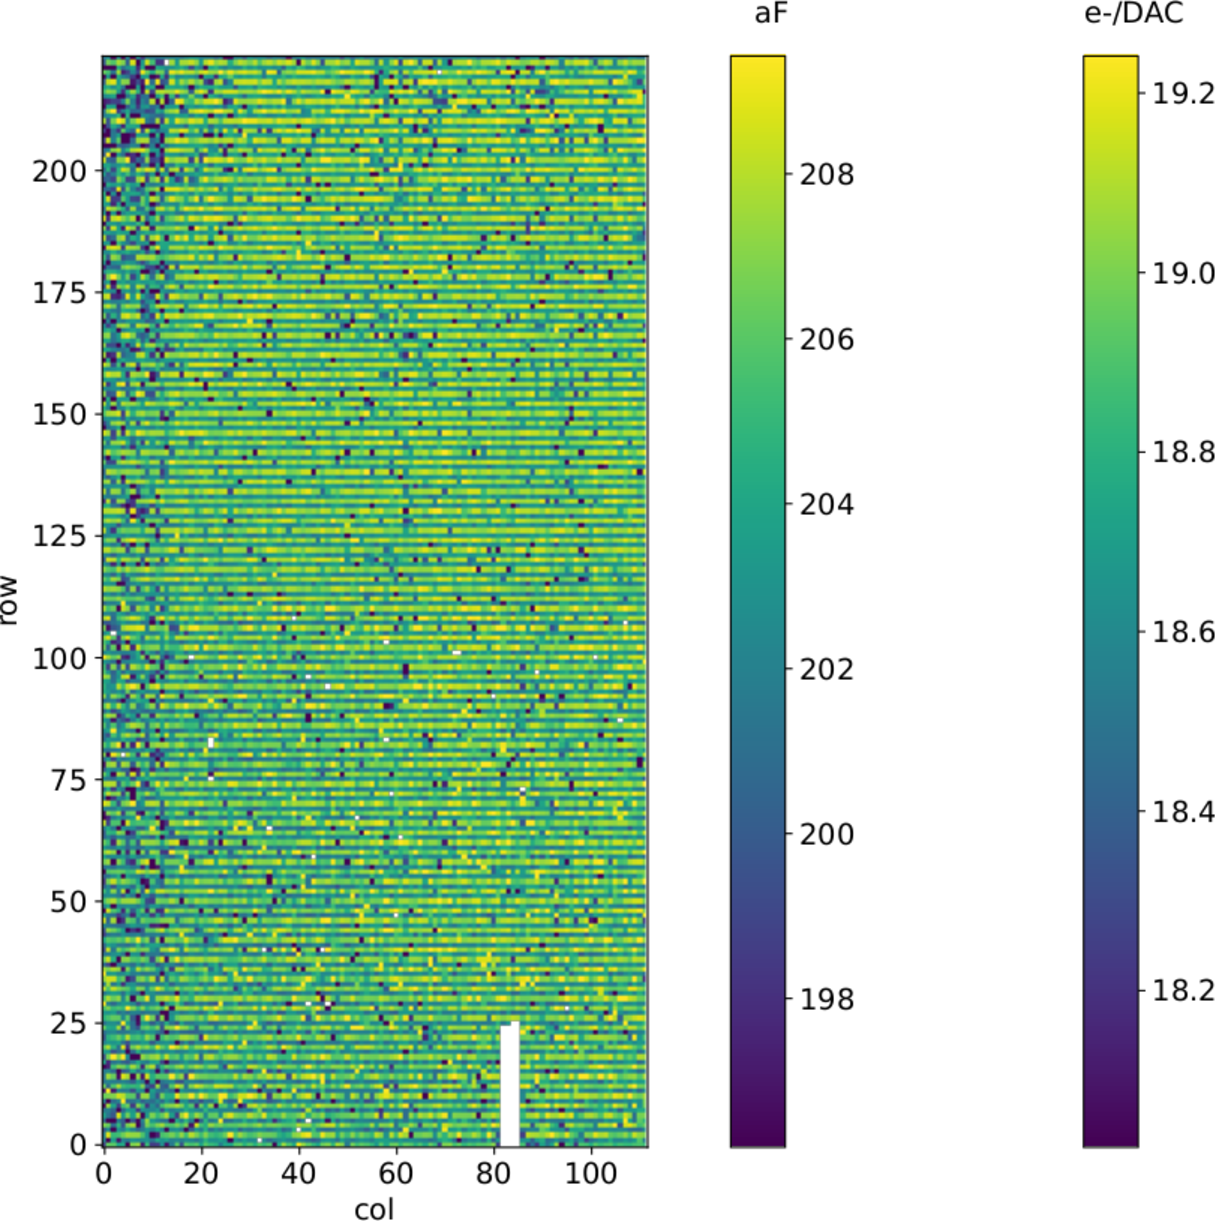
\includegraphics[width=.49\linewidth]{figures/charaterization/conversion_factor_map.pdf}
            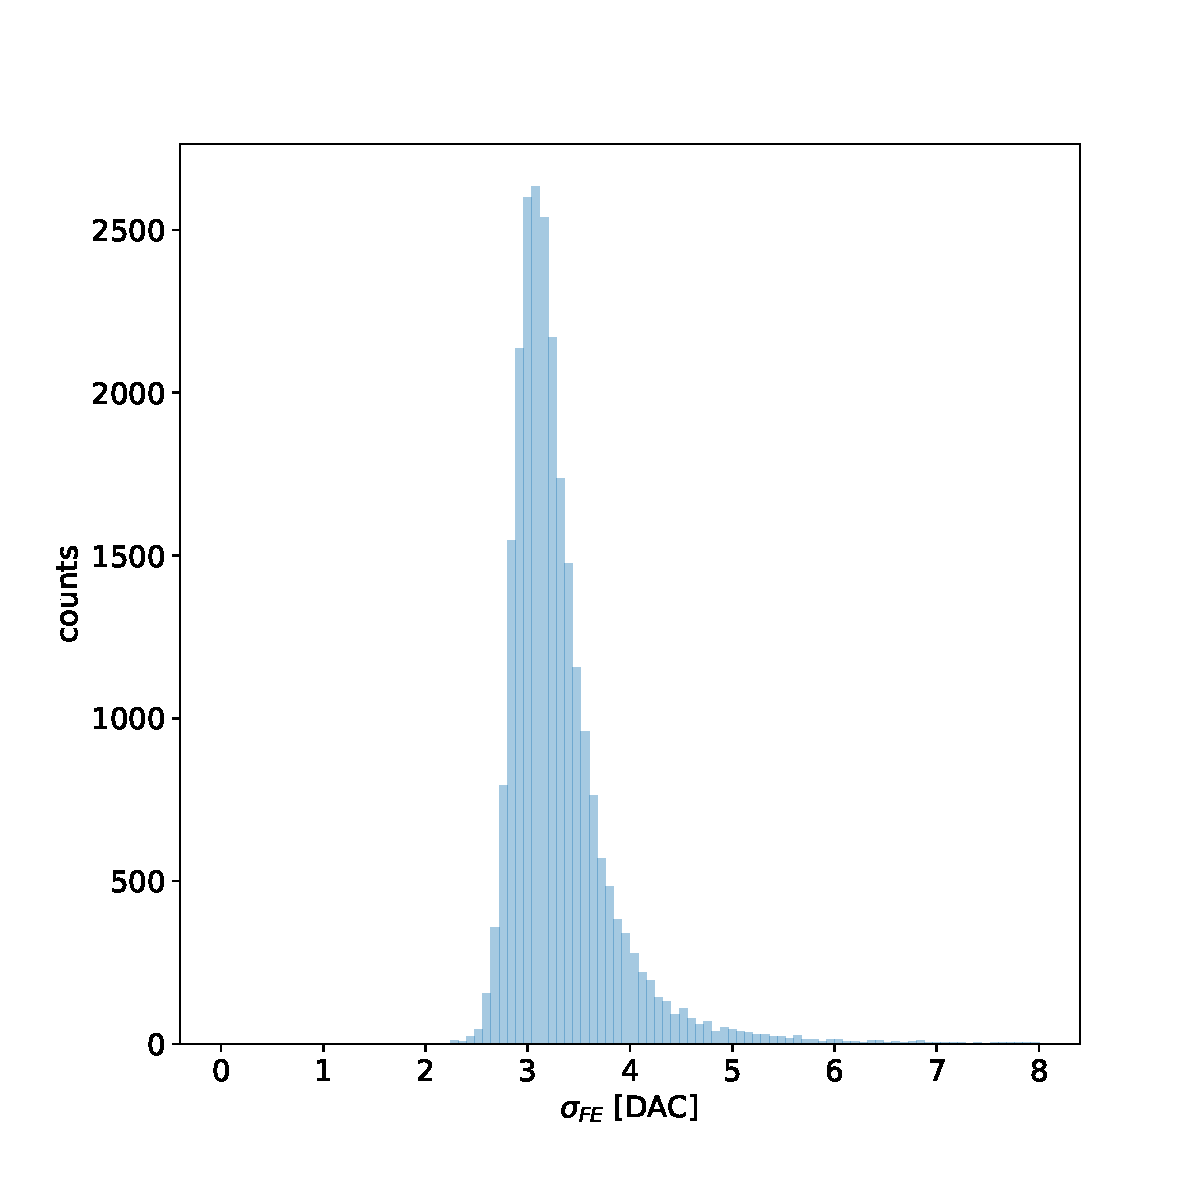
\includegraphics[width=.49\linewidth]{figures/charaterization/Fe_width_DAC_hist.pdf}            
            \label{fig:}
            \caption{}
        \end{figure}         


    \subsection{Changing the bias}\label{chap:characterization_section:bias}
        In order to study the behavior of the sensor changing the bias, I perform some injection scans in different configurations. 
        The thickness of the depletion has to be considered indeed an important parameters for the efficiency of the signal, and in particular it affects the charge released by a particle which cross the sensor (since the signal is proportional to the thickness of the epitaxial layer).
        Given that the chip under examination has a gap in the low dose epi-layer (look at chapter \ref{chapter:TJMonopix1_thesensor}) we were not able to change independently the bias of the substrate (PSUB) and of the p-well (PWELL), but they must be kept at the same value, differently from other chips, where on which some test has been performed, as reported in figure \ref{fig:gain_vs_bias}.
        A 2D map of the measured output voltage amplitude and resulting gain in the case of the PMOS and HV are reported. 
        \begin{figure}[h!]
            \centering
            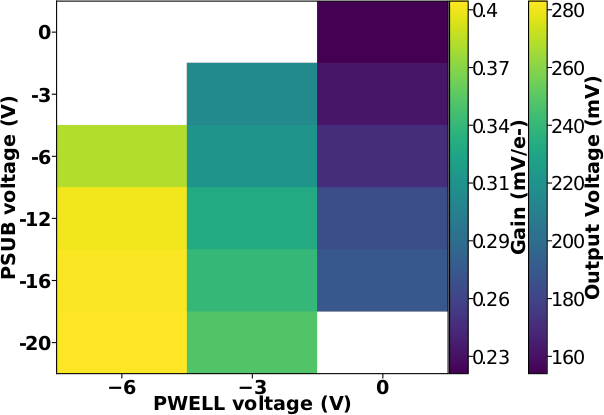
\includegraphics[width=.45\linewidth]{figures/Monopix1/PMOS_gain_bias.png}
            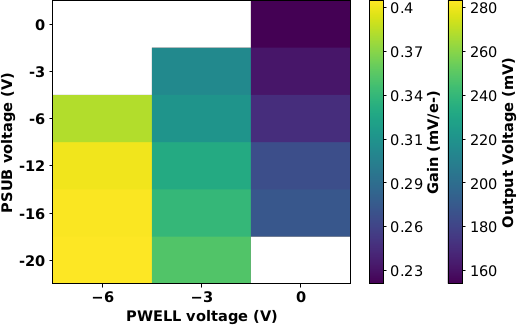
\includegraphics[width=.49\linewidth]{figures/Monopix1/HV_gain_bias.png}            
            \caption{2D map of the output voltage amplitude and gain with respect to the p-well and p-substrate in the case of the PMOS reset front-end (B)}
            \label{fig:gain_vs_bias}
        \end{figure}  

        In order to test the behavior of the chip when not completely depleted, I have performed an injection scan with PSUB/PWELL bias at \SI{0}{V}, -\SI{3}{V} and -\SI{6}{V}, and some acquisitions with the Fe55 source.
        The results of the measurements are reported in table \ref{tab:parameters_vs_bias} and in figure \ref{fig:Fe_spectrum_bias}.
        Turning down the bias, the depletion region narrows and the efficiency reduces, in particular in the pixel corner; in particular the threshold increases of $\sim$1/4, the noise of $\sim$1/3 and the slope, which parameterizes the linearity of the analog output and strictly depends on the gain, decreases of $\sim$1/4.
        In figure \ref{fig:Fe_param_vs_bias}(b) are reported the values of the K$_\alpha$ peak position, the normalization of the events above the peak and the rate, everything has been normalized to the value at the reference condition, which is with PSUB/PWELL at -\SI{6}{V}. 
        In order to evaluete the peak position and the normalization I have fit the spectrum in the region on the right with a gaussian.
        Looking at the spectrum, an other characteristics seems to appear: at lower bias the peak width is bigger than in a full depletion mode.
        This could be due at a bigger capacity, which influence the noise.         
    \begin{table}
            \begin{center}
            \begin{tabular}{| c |  c | c | c |}
            \hline
               & -\SI{6}{V} & -\SI{3}{V} & \SI{0}{V}\\
            \hline
            \hline
            Threshold [DAC] & 20.04 $\pm$ 1.6 & 21.0 $\pm$ 1.6 & 24.5 $\pm$ 1.8\\
            Noise [DAC] & 0.613 $\pm$ 0.075 & 0.625 $\pm$ 0.078 & 0.822 $\pm$ 0.098\\
            Slope [au/DAC] & 0.726 $\pm$ 0.027 & 0.707 $\pm$ 0.028  & 0.573 $\pm$ 0.021\\
            Offset [au] & -10.8 $\pm$ 1.9 & -11.2 $\pm$ 1.8 & -11.1 $\pm$ 1.5 \\
            \hline
            \end{tabular}
            \caption{The errors are the standard deviations of the corresponding distributions. The conversion factor from DAC to electrons is $\sim$\SI{20}{e-/DAC}.}
            \label{tab:parameters_vs_bias}
            \end{center}
        \end{table}  
        
        \begin{figure}[h!]
            \centering
            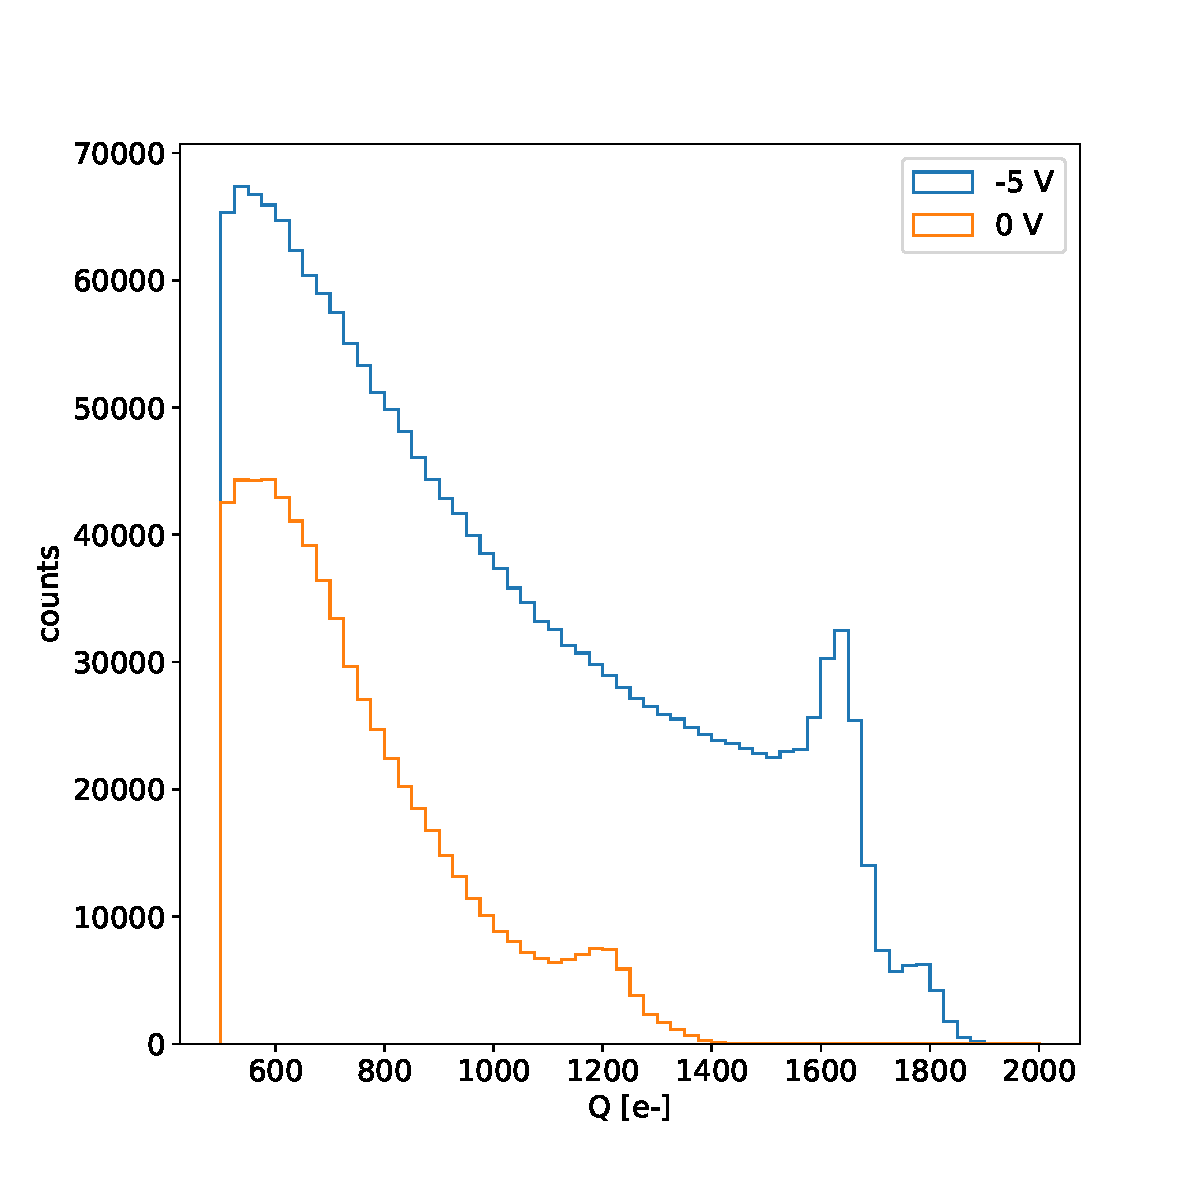
\includegraphics[width=.60\linewidth]{figures/charaterization/Fe_spectrum_bias.pdf}
            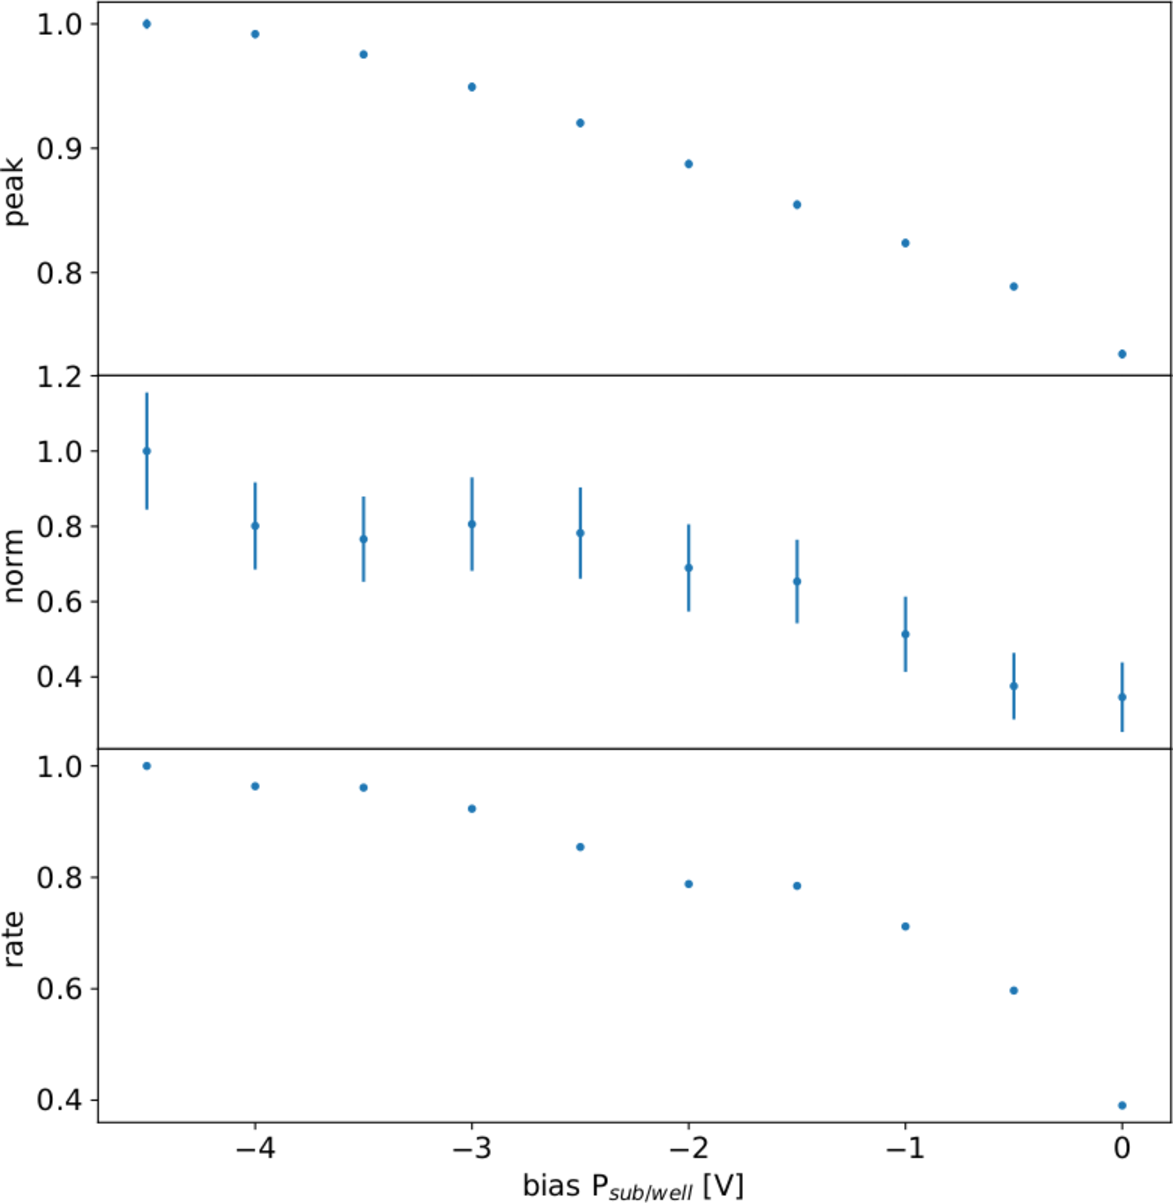
\includegraphics[width=.70\linewidth]{figures/charaterization/Fe_param_vs_bias.pdf}
            \caption{Two acquisition with the Fe55 source at different bias. }
            \label{fig:Fe_param_vs_bias}
        \end{figure}     


    \subsection{Measurements with radioactive sources}
        %python3 -i acquisition_Fe55/find_cluster.py -d acquisition_Fe55/source_PMOSS/noise_acquisitions_6V -> per cluster dimension e spettro del noise
        %python3 -i acquisition_Fe55/hit_map.py -f acquisition_Fe55/source_PMOSS/2022-04-07/2022-04-07_10-10-01_acq.h5 -> per le hit map, comprese qualche hitmap dei cluster
        %python3 -i acquisition_Fe55/Sr90_spectrum.py -d acquisition_Fe55/source_PMOSS/noise_acquisitions_6V/ -> per fare i plot dello stronzio
        In order to completely validate the operation of the whole sensor\footnote{As I will explained in chapter \ref{chap:} these measurements are foundamental also to be compared with the spectrum seen at the testbeam}, I have made some acquisitions with radioactive source, in particular I have used Fe55, Sr90, which is a $\beta^-$ emettitor with electron endpoint at \SI{0.546}{MeV}, and cosmic rays, which are supposed to be mostly MIP. 
        In the acquisitions with Sr90 and cosmic rays, I specifically focused on the events whith charge sharing and with more hits than one per events, that are clusters.

        The definition of cluster I chose is built only on the time of arrival of hit, in particular I established that all particles with the same timestamp belong to the same cluster.
        This obviously is a coarse requirement but it gave me the opportunity of using a simple and fast clustering algorithm, which is fine when the random coincidence probability is neglibile. 
        Defining R$_1$ and R$_2$ as the two events rate, and $\tau$ as the dead time of the detector, the random coincidence rate can be found: 
        \begin{equation}
            R_{coinc} = R_1 \, \times\, R_2 \, \times \, \tau
        \end{equation}
        As I am going to prove in the next section, the dead time strictly depends on the occupancy of the matrix, even through we can assume a dead time of $\sim$\SI{1}{\um}, which corresponds to the mean dead time per pixel. However, if in an event a particle hit two different pixels producing a cluster, the total dead time simply doubles.   
        Then, assuming a rate of noise of $\sim$\si{Hz} on the whole matrix and being the mean rate of the , the random coincidence of two hits coming from Fe-noise, Sr-noise, CR-noise and noise-noise are respectively 
        
        In figure \ref{fig:cluster_dimensions} I report the histograms of the number of pixels in the cluster and of the dimension of clusters, defined in terms of the max and min coordinates on the matrix as:
        \begin{equation}
            d = \sqrt{(y_{max}-y_{min})^2 + (x_{max}-x_{min})^2}
        \end{equation}
        \red{quello che si nota è che lo Sr  fa cluster più grandi mediamente, che arrivano anche a 22 hit.}

        Below I have also attached a sample of hitmap of events produced by the three different sources. 


        \begin{figure}[h!]
            \centering
            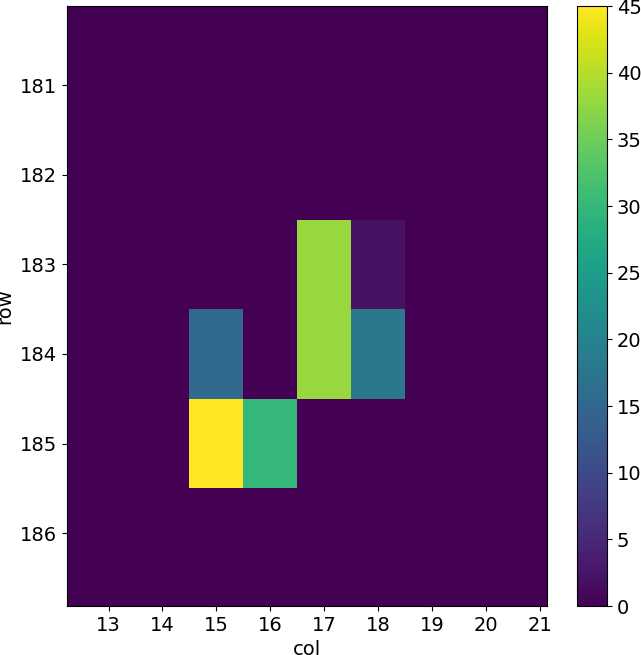
\includegraphics[width=.24\linewidth]{figures/charaterization/evts/cosmic_rays/7a.png}
            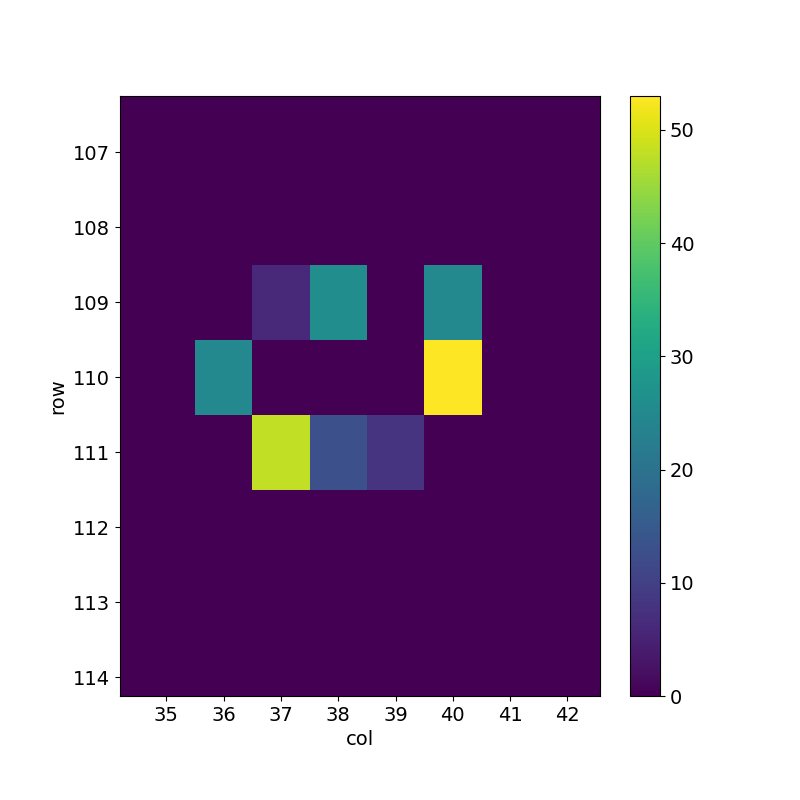
\includegraphics[width=.24\linewidth]{figures/charaterization/evts/cosmic_rays/8a.png}
            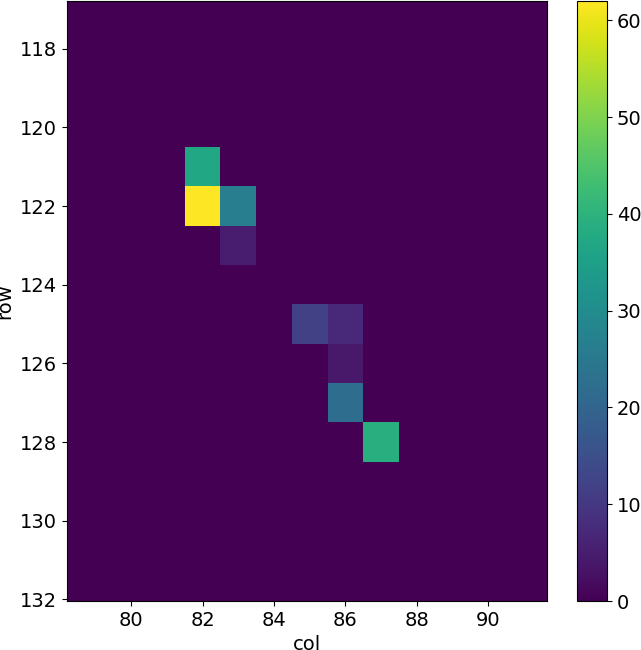
\includegraphics[width=.24\linewidth]{figures/charaterization/evts/cosmic_rays/9c.png}\\       
            \includegraphics[width=.24\linewidth]{figures/charaterization/evts/cosmic_rays/10a.png}
            \includegraphics[width=.24\linewidth]{figures/charaterization/evts/cosmic_rays/11a.png}
            \includegraphics[width=.24\linewidth]{figures/charaterization/evts/cosmic_rays/12.png}
            \includegraphics[width=.24\linewidth]{figures/charaterization/evts/cosmic_rays/12b.png}               
            \caption{ }
            \label{fig:hit_map_cosmic_rays}
        \end{figure} 


        \begin{figure}[h!]
            \centering
            \includegraphics[width=.24\linewidth]{figures/charaterization/evts/Sr90/9b.png}
            \includegraphics[width=.24\linewidth]{figures/charaterization/evts/Sr90/10b.png}
            \includegraphics[width=.24\linewidth]{figures/charaterization/evts/Sr90/13a.png}
            \includegraphics[width=.24\linewidth]{figures/charaterization/evts/Sr90/16a.png}\\
            \includegraphics[width=.24\linewidth]{figures/charaterization/evts/Sr90/18b.png}
            \includegraphics[width=.24\linewidth]{figures/charaterization/evts/Sr90/21a.png}
            \includegraphics[width=.24\linewidth]{figures/charaterization/evts/Sr90/22a.png}
            \includegraphics[width=.24\linewidth]{figures/charaterization/evts/Sr90/25a.png}               
            \caption{ }
            \label{fig:hit_map_Sr90}
        \end{figure}         

        \begin{itemize}
            \item PLOT delle hit per cluster
            \item  esempio di hitmap di cluster
            \item sostituisci in carica in un file del ferro, guarda somma dei cluster, stessa cosa per Sr e MIP
            \item  Spiega che con il flavor HV abbiamo una perdita di sengnale, fai vedere uno spettro di delle misure dell 8 marzo. 
        \end{itemize}
        The signal generated by electrons is similar to the one generated by minimum ionizing particle (MIPS) \red{dovrei mettere qualche conto per giustificare questa affermazione}, and the spectrum is expected to follow a Langau-Gauss distribution.
        \red{nelle acquisizioni dei CR ho selezionato solo i cluster, per tagliare via il rumore.}
        
        , looking at the cluster dimension and the cluster charge.  


    \subsection{Dead time measurements}
        The hit loss is due to analog and digital pile up: the first one occurs when a new hit arrives during the pre-amplifier response, the second instead when the hit arrives while the information of the previous hit has not yet been transferred to the periphery.  
        Since the pre-amplifier response has a characteristic time $\sim$ToT, the dead time $\tau_{a}$ introduced by it will be at most \SI{1.6}{\us}; using the IRESET and VRESET FE parameters the reset time can be lowered down, but a \red{IRESET, puoi diminuire il tempo di scarica.}   
        Regarding the latter contribution instead, since only one hit at a time can be stored on the pixel's RAM, until the data have completed the path to get out, the pixel is paralyzed. Moreover since there is no storage memory included on TJ-Monopix1 prototypes, the digital dead time $\tau_{d}$ almost corresponds to the time needed to trasmit the data-packets off-chip. 

        The exportation of data from pixel to the EoC occurs via a 21-bits data bus, therefore only one clock cycle is needed and the dead time bottleneck is rather given by the bandwidth of the serializer which trasmits data off-chip from the EoC. In our setup the serializer operates at 40 MHz, thus to transmit a data packet (27-bit considering the addition of 6 bits to identify the double-column at the EoC) at least \SI{675}{ns} are needed. 
        For what we have said so far, the R/O is completely sequential and therefore is expected a linear dependence of the reading time on the number of pixels to read:
        \begin{equation}
            \tau =\, 25\: \unit{ns}\, \times\, (\alpha\, N +\, \beta)
            \label{eq:reading_time}
        \end{equation}
        where $\alpha$ and $\beta$ are parameters dependent on the readout chain setting. 
        
        To test the linearity of the reading time with the number of pixels firing and to measure it, I have used the injection circuit which allows me choosing a specific hit rate: I made a scan injecting a fix number of pulses and each time changing the number of pixels injected.
        Indeed the injection mode allows fixing not only the amplitude of the pulse, which corresponds to the charge in DAC units, but also the time between to consecutive pulses (DELAY) and the width (WIDTH). The hit rate then corresponds to :
        \begin{equation}
            R = \frac{\SI{25}{ns}}{(DELAY+WIDTH)}
        \end{equation}
        where WIDTH is equal to \SI{60}{counts}. 

        Unfortunately a high random hit rate on the matrix cannot be simulated by the injection because of the long time ($\sim$\si{ms}) needed to set the pixel registers of the injection; then I was forced to specify at the start of the acquisition the pixels to inject on, and for convenience I chose those on a same column.  
        In figure \ref{fig:efficiency_VS_delay} is shown the dependence of the efficiency on the DELAY parameter in two different cases. 
        For the 5 pixels example the efficiency goes down the 90\% at a DELAY of $\sim$185 clock counts, which corresponds to \SI{6.125}{\us} and to a rate of \SI{160}{kHz}, while in the 10 pixels example, the efficiency goes under the 100\% at $\sim$\SI{380}{clock} counts, which corresponds to \SI{11}{\us} and to a rate of \SI{90}{kHz}. 
        \red{COME MAI SONO DIVERSE LE CURVE?}
        \begin{figure}[h!]
            \includegraphics[width=.49\linewidth]{figures/charaterization/efficiency_5pixels.png}
            \centering
            \includegraphics[width=.49\linewidth]{figures/charaterization/efficiency_10pixels.png}
            \caption{Efficiency vs the DELAY parameters. (a) I made a scan injecting 5 pixels with 50 pulses for each DELAY configuration and (b) 10 pixels with 100 pulses for each DELAY}
            \label{fig:efficiency_VS_delay}
        \end{figure}
        From the efficiency curves I have then looked for the time when the efficency decreases. In figure \ref{fig:dead_time}(a) is shown the dead time per pixels as a function of N with different R/O parameters configuration, the meaning of which is explained in chapter \ref{chap:Monopix_RO}. The default value suggested by the designer of the chip are reported in table \ref{tab:R/O_param}; moving too much the readout parameters from the default ones, the readout does not work properly, and no hits can be read at all. The problem probably stays in the firmware setting of the readout which are specially fixed for our chip \red{Sul repositorio, nei commenti ci sono altri valori possibili per il FREEZE, ma avevamo detto che probabilmente sono relativi ai setting di altri chip.}
        %Cambiando molto i parametri del R/O la lettura non funzionava per niente: ad esempio CONF\_STOP\_FREEZE non può essere impostato nè sopra 105 nè sotto 95
        Despite the single pixel reading time does not depend on the position on the pixel matrix, whithin a clock count which is $\sim$\SI{25}{ns}, and it is equal to \SI{106}{clock} counts, since the $\tau_d$ critically depends on the pixel position on the matrix: in particular the reading sequence goes from row 224 to row 0, and from column 0 to column 112, making the pixel on the bottom right corner the one with the longest dead time. 
       
        \begin{table}
            \begin{center}
            \begin{tabular}{|c | c | c |}
            \hline
            Parameter & Value [\si{DAC}] & Value [\si{\us}]\\
            \hline
            \hline
            START\_FREEZE & 64 & 1.6\\
            STOP\_FREEZE & 100 & 2.5\\
            START\_READ & 66 & 1.65\\
            STOP\_READ & 68 & 1.7\\
            \hline
            \end{tabular}
            \caption{Default configuation of the R/O parameters}
            \label{tab:R/O_param}
            \end{center}
        \end{table}
        \begin{figure}[h!]
            \centering
            \includegraphics[width=.9\linewidth]{figures/charaterization/parameters_points.png}
            \includegraphics[width=.9\linewidth]{figures/charaterization/default_line.png}
            \caption{(a) Readout time per pixel as a function of the number of pixel injected obtained with different FE setup. (b) Readout time as a function of the number of pixels injected obtained injecting pulses with amplitude of \SI{80}{DAC} (green), of \SI{40}{DAC} on the same row (red) and on the same column (blue).}
            \label{fig:dead_time}
        \end{figure}
        Furthermore to test that there is no dependece of the digital readout time from the charge of the pulse, I have try to change the amplitude of the pulse injected, but the parameters found were consistent with the default configuration ones.
        No difference in the $\alpha$ and $\beta$ coefficients has been observed between the two case.
        \red{In realtà non mi torna perchè il FREEZE dovrebbe iniziare n cicli di clock dopo il TE, ed il TE dipende ovviamente dal ToT, quindi mi sarei aspetatta una differenza tra i due.}
        Referring to eq.\ref{eq:reading_time}, the factor $\alpha$ is proportional to the difference (STOP\_FREEZE - START\_READ), while the offset $\beta$ lies between 5 and 15 clock counts.

        Per avere una misura veritiera del tempo morto e del hit loss si dovrebbe iniettare casualmente input events are produced by a
        random hit generator with a specified hit rate, hence following a Poisson distribution. Inoltre faccio notare che il tempo morto è così lungo perchè c'è parallelizzazione e neppure un buffer (cosa tipicamente prevista quando li si inserisce nei rivaltori). Ad esempio Obelix, per l'upgrade di Belle2 avrà un buffer a fine matrice. 

\section{ARCADIA-MD1 characterization}
    Unfortunatly we have found out that the chip we received was not completely functional, then we have been able to make on it only a few electrical and software test. We have then verified the comunication of the chip with the DAQ, testing the operations of the FPGA and the breackout board (BB).  
    The problem occurs when the chip is biased, in particular, when the HV voltage is lowered down \SI{0}{V}, the sensor requires too much power and a too high current draw sets. We have discussed the problem with the designers of the chip whose helped us indentifying the motivation of the break: the chip has been glued using too much conductive tape and hence have a short-circuit between the sides and the back, which makes impossible the biasing.     
    Unfortunately, since both the sensor and the FE require at least -\SI{10}{V} to work properly, no measurement was possible except the acquisition of the noise in the FE circuit. 
    \begin{figure}[h!]
        \centering
        \includegraphics[width=.95\linewidth]{figures/charaterization/ARCADIA/pixel_per_row_per_acq_11_60.png}
        \caption{Noise in the front end circuit depending on the bias road across the matrix was recorded. }
        \label{fig:ARCADIA_threshold}
    \end{figure}

    %   Non ero entrata in dettaglio a proposito del baco perché non mi sembrava rilevante, ma non ho nessun problema a farlo ora. Durante la seconda sottomissione ci siamo accorti che il segnale che abilita i drivers LVDS delle sezioni aveva polarità sbagliata. I drivers LVDS sono quei circuiti che pilotano i dati verso il mondo esterno e avere un enable di polarità errata significa che i drivers risultano sempre spenti durante l'acquisizione. Quindi in pratica il chip funziona, ma non è in grado di trasmettere nulla all'esterno. Il segnale di enable viene controllato internamente al chip dalla logica di periferia e non è direttamente accessibile da fuori. Fortunatamente le linee di metallo che pilotano il suddetto segnale sono in una regione del chip poco densa, cioè senza altro metallo sopra e attorno. E' stato quindi possibile intervenire con un fascio di ioni focalizzato per andare a scavare nelle regioni di interesse fino ad accedere ai segnali di enable. Abbiamo quindi tagliato la connessione interna e cortocircuitato l'enable  al valore di tensione corretto.  Nel minid 2 questa correzione è stata fatta sul chip ed è l'unica modifica rispetto alla prima sottomissione.


    % Threshold (electrons):
    %   VCASN  |   e-
    %----------------
    %      0    | fe off
    %      1    |  835
    %      4    |  625
    %      7    |  475
    %      10   |  400
    %      16   |  360
    %      25   |  290
    %      31   |  220
    %      37   |  145
    %      ...
    %      63   |  min

    We received then another chip, a minid2, that is a "mini demonstrator" from the second submission. The two chips have the same charateristics but the minid2 is smaller than the MD1, in particular it only have 32$\times$512 pixels, instead of 512$\times$512.  
    \red{scrivi il problema della prima sottomissione.}


    An exhaustive characterization and testing of the new chip have been going on in the clean room on the INFN, and I am going to show here only some preliminary results.
    Up to now we used the injection circuit in order to make a threshold scan on a few pixels: differently from the TJ-Monopix1's charaterization where we performed a scan changing the injection charge of the pulse, with the minid2 we have instead changed the threshold (whose register is VCASN) keeping the charge of the pulse fixed.
    For each threshold we inject 100 pulses of amplitude \SI{10}{\us}. The dependece of the efficiency on the threshold for two pixels is shown in figure \ref{fig:ARCADIA_threshold}.  
    \begin{figure}[h!]
        \centering
        \includegraphics[width=.7\linewidth]{figures/charaterization/ARCADIA/threshold_0_0.pdf}
        \caption{}
        \label{fig:ARCADIA_threshold}
    \end{figure} 
    
    \red{Anche se il comportamento è globalmente ragionevole, con l'efficienza che sale quando si abbassa la soglia, viene il sospetto che non stiamo polarizzando bene il sensore e il FE dato che anche raggiunto i centi conteggi, si hanno delle fluttuazioni intorno a questo valore. Inoltre notiamo che abbassando ulteriormente la soglia si osserva un aumento delle hit, dovuto al fatto che si inizia a triggerare sul rumore. }

    \red{commenta sul fatto che non è stabile anche molto sopra la soglia. Forse è dovuto al bias? oppure l 'impulso ha qualche problema (non abbiamo settato la durata ecc..)? Che valore ha in elettroni?}

    Substantial differences have been observed in both the efficiency and the threshold among the sections, with VCASN=\SI{40}{DAC}; this suggests that with this particular FE configuration there is a big threshold dispersion on the matrix.  
    The hitmap of an acquisition with the Fe55 source is shown in figure \ref{fig:ARCADIA_Fe55}: the whole MD1 matrix with only the bottom region (32 rows) working is represented in (a), while in (b) there is a zoomed hitmap. The rate seen within the region 8 (green region in the figure (a)) is compatible with the rate of the same radioactive source measured with TJ-Monopix1, that it $\sim$\SI{3.3}{kHz}. 
    \begin{figure}[h!]
        \centering
        \includegraphics[width=.49\linewidth]{figures/charaterization/ARCADIA/Fe55_5min30s.png}
        \includegraphics[width=.47\linewidth]{figures/charaterization/ARCADIA/Fe55_6min30s.png}
        \caption{Fe55 acquisition with VCASN=\SI{40}{DAC}. (a) All the matrix 512$\times$512 is plotted even if the minid2 has only the rows in range 0-32. (b) A zoom on the first section (col 0-32).   }
        \label{fig:ARCADIA_Fe55}
    \end{figure}  
    Looking to the Sr90 acquisitions (fig.\ref{fig:ARCADIA_Sr90}) many clusters and tracks can be immidiately distiguished, confirming what observed with TJ-Monopix1. 
    \begin{figure}[h!]
        \centering
        %\includegraphics[width=.49\linewidth]{figures/charaterization/ARCADIA/Fe55_9min.pdf}
        \includegraphics[width=.7\linewidth]{figures/charaterization/ARCADIA/Sr90_2min.pdf}
        \caption{Sr90 acquisition with VCASN=\SI{40}{DAC}. The different colours are related with the time of arrival of the hits: in yellow the most recent hits, while in blue the old ones.}
        \label{fig:ARCADIA_Sr90}
    \end{figure}  

    %test_play_wip.py,
    % example/test_initialization.py
    %example/test_play_triggered_wip.py 






\chapter{Test beam measurements}
During August 2022 a testbeam took place in Santa Chiara hospital in Pisa, where a new accelerator designed for both medical research and R$\&$D on FLASH-RT, and for this reason called "ElectronFlash", have been installed a few months ago. 
The motivation of the testbeam measurements were testing TJ-Mopopix1 at high dose rate with a focus on investigating the possibility of the application in radiotherapy. Despite this particular device does not seem fitting the requirements imposed for that application, especially regarding the readout time, the measurements have been useful since help us charaterizing the setup for future advance, and also give us the possibility of a complete charaterization of the chip.

Given that in medical physics the dose is the standard parameter to charaterize the beam, beacause of its obvious relation with the damage caused in the patient, I am going to explain the meaning of it by the point of view of the instrumentation.
Infact, when interacting with measuring systems a more common and usefull parameter is the rate or the fluence of particles.
The conversion between the two quantity can be find thinking to the definition of dose: it is the concentration of energy deposited in tissue as a result of an exposure to ionizing radiation. 
Assuming total absorption of electrons in water, defined by law as the ordinarily reference medium, the dose can be expressed as: 
\begin{equation}
   D[Gy] = \frac{N E[eV]}{\rho[g/cm^3] A[cm^2] x[cm]}
\end{equation}
After having applyed the conversion of the energy from \si{eV} to \si{J} and noticed that E/$\rho$x roughly corresponds to the stopping power S of electrons in water, a simple estimation of the dose released in water is:
\begin{equation}
   D[Gy] = 1.602\;10^{-10}\,N[cm^{-2}]\,S[MeV cm^2/g]
\end{equation}


\section{Apparatus description}
   In order to shield the outdoor from ionizing radiation the accelerator is placed in a bunker inside the hospital. The bunker has very thick walls of cementum and both the control units of the accelerator and of the detector were placed outside in a neighbor room. 
   \subsection{Accelerator}
      \begin{figure}
         \centering
         \includegraphics[width=.9\linewidth]{figures/test_beam/beam_structure.pdf}
         \caption{Typical beam structure of a beam with the standard characteristic quantity}
         \label{fig:beam_structure}
      \end{figure}
      \begin{table}
         \begin{center}
         \begin{tabular}{| c | c | c |}
         \hline
      $\bar{D}$ & Dose rate (mean dose rate for a multi-pulse delivery) & 0.005-10000 Gy/s\\
      $\Dot{\bar{D}}$ & Intra pulse dose rate (dose rate in a single pulse) &  0.01-1 10$^6$ Gy/s  \\
      DDP & Dose in a single pulse & 0.04-40 Gy\\
      PRF & Pulse repetition frequency(number of pulses delivered per unit of time) & 1-350 Hz\\
      t$_{p}$ & Pulse width & 0.2-4 \si{\us}\\
      n & Number of pulses & single/pulse train \\
      \hline
         \end{tabular}
         \caption{The parameters that can actually be set by the control unit are the PRF, DDP, t$_p$ and n (in particular singolar irradiation or pulse train), while the other changes consequently.}
         \label{tab:beam_parameters}
         \end{center}
      \end{table}  
      The ElectronFlash accelerator is an electron Linear Accelerator (LINAC) with two energy configurations, at \SI{7}{MeV} and \SI{9}{MeV}, and it can reach ultra high intensity (\SI{40}{Gy/pulse}) keeping the possibility of accessing many different beam parameters and changing them independently from each other, a characteristic that makes it almost unique worldwide and which is faundamental for research in FLASH-RT, both for the medical aspects\footnote{For example, it is not yet really clear the dependence of the efficacy of the FLASH effect on the whole beam parameters} and for the studies on detectors. 
      The accelerator implements the standard beam structure used in RT with electrons (fig. \ref{fig:beam_structure}), that is a macro pulse divided in many micropulses; the parameters used to set the dose and their range of values settable by the control unit is reported in table \ref{tab:beam_parameters}. 

      The accelerator is also provided of a set of triod cannons $\sim$\SI{1.2}{m} long and with diameters in range from \SI{1}{cm} to \SI{12}{cm} and a collimator that can be used as beam shaper to produce a squircle shape.
      The triode, which is made by plexiglass, must be fix to the gun during the irradiation and is needed for producing,  via the scattering of electrons with it, an uniform dose profile (fig.\ref{fig:dose_profile}) which is desired for medical pourpose.
      \begin{figure}[h!]
         \centering
         \includegraphics[width=.49\linewidth]{figures/test_beam/dose_profile_10cm.pdf}
         \includegraphics[width=.49\linewidth]{figures/test_beam/dose_profile_1cm.pdf}
         \caption{Two example of x-y isodose curves for two different triodes, \SI{10}{cm} and \SI{1}{cm} respectively, reported by the producer in the manual with the specific of the accelerator (S.I.T. - Sordina IORT Technologies S.p.A.). With the smaller collimator the dose rate in pulse is comparatively higher.}
         \label{fig:dose_profile}
      \end{figure}  

   \subsection{Mechanical carriers}
      The tested detector consists in one chip, the Device Under Test (DUT), mounted on a board and connected to FPGA with same arrangement of figure \ref{fig:}.
      These boards have been positioned vertically in front of the triode on a table specifically built for the testbeam. The tree board have been enclosed in a box of alluminium with a window on the DUT and with the required holes at the side to enable the biasing via cables and the connection with the DAQ provided via ethernet cable.       
      A trigger signal coming from the control unity and syncronized with the pulses emitted from the beam has been also sent to the FPGA.
      This digital signal cannot be considered a real trigger, since the TJ-Monopix1 prototype has been designed to be triggerless, but its Time of Arrival (ToA) had allowed the reconstruction of the correct timing during the analysis.

      In order to shield the sensor from the whole particles emitted from the gun, two alluminium collimators have been fabricated: one has been positioned at the triode exit while the other in front of the DUT. The collimators are $t$=\SI{32}{mm} thick and have a diameter $d$ equal to \SI{1}{mm}: assuming a beam divergence bigger than $d/t$=1/32 = \SI{1.8}{\degree}, which is the case, the collimator at the triode output was supposed to work as a point source and to reduce the rate on the DUT of a factor at least 4 10${^-4}$. The second one, being near the DUT, was instead supposed to shield the sensor from the electrons which have passed the first one, except for a region of \SI{1}{mm\squared} configurable using \red{come si chiamano quei cacciavitini per settare la posizione? sliding trimmer?}.  
      \begin{figure}[h!]
         \centering
         \includegraphics[width=.40\linewidth]{figures/test_beam/electron_flash.jpg}
         \includegraphics[width=.35\linewidth]{figures/test_beam/collimator_box.jpg}\\     
         \includegraphics[width=.77\linewidth]{figures/test_beam/carrello.jpeg} 
         \label{fig:set_up}
         \caption{Experimental set up. (a) ElectronFlash accelerator: a
         rotating gantry allows the gun orientation from \SIrange{0}{90}{\degree} (horizontal /vertical). (b) Collimator and DUT box. (c) Whole structure mounted: we used the \SI{10}{cm} diameter and \SI{1.2}{m} long triode; the DUT which is in the box behind the two collimators is connected to the power supply units.}
      \end{figure}  

\section{Measurements}
   Because of the dead time of TJ-Monopix1 it is not possible resolving the bunch sub-structure and almost no one pixel can read more than a hit per bunch. I recall, indeed, that the dead time per pixel depends on the location on the priority chain for the readout and for each pixel $\lesssim$\SI{1}{\us} (fig. \ref{fig:}) are needed; therefore only a few pixels at the top of the priority chain (at the upper left of the matrix) can fire a second time, since they in principle can be read the first time before the end of the pulse (assuming a pulse duration in \SI{2}{\us}-\SI{4}{\us}) and then can be hit again.

   Since resolving the single electron track is impossible, a way this sensor could be used in such context is reducing its efficiency and taking advantage of the analog pile up and of the linearity of the analog output (ToT), in order to see a signal produced not by the single particle but by more electrons. 
   Reducing the efficiency and the sensibility of the sensor is essential in order to decrease the high charge signal produced in the epitaxial layer: if the sensor is completely depleted the collection efficiency is closer to 1\% and if the whole charges produced by a MIP, \SI{80}{e-/\um} about, are collected, the saturation limit is soon reach. Then a condition where there is a partial recombination of the center electron-hole created in the bulk is desiderable.
   On the other hand, the smaller the output signal value and the higher the rate the detector can cope with: indeed, the rollover constitutes a limit for the usage of the analog output. 
   With the standard configuration of the FE parameters and the epitaxial layer completely depleted, a MIP produces a ToT out of range of representation of 6-bit; 
   so as to obtain smaller output signals one can operate on the reduction of the gain of the preamplifier or on the pulse velocity of returnig to the baseline. 
   Recalling the results in section \ref{chap:characterization_section:bias}, I have shown that concerning the PMOS flavor 1, reducing the bias from -\SI{6}{V} to \SI{0}{V} brings a reduction of efficiency down to \SI{40}{\%}, and a reduction in the gain of a factor $\sim$1/3, while the reduction of the gain of the preamplifier allows a reduction of \red{circa 10, ma da controllare}.
   
   In order to taking advantage of the analog pile up and integrating the charge, for semplicity assume of two electrons, the second one must hit the pixel before the ToT goes under the threshold. The general condition is then $\overline{\Delta T}<\overline{ToT}$, but if a high P$_\mu$($n\geqslant$1) is required, a lower $\overline{\Delta T}$ may be desired:
   \begin{equation}
      P(n\geqslant1) = \sum\limits_{n=1}^n \frac{e^{-\mu\;\mu^n}}{n!} = 1\;-\;P(0) = 1\;-\;e^{-\mu}
   \end{equation}
   \begin{equation}
      \mu = \frac{\overline{ToT}}{\overline{\Delta T}}
   \end{equation}
   If a P$_\mu$($n\geqslant$1) = 99\% then the $\overline{\Delta T}$ must be $\sim$0.22$\overline{ToT}$. The ToT is in range [0,64] but since the rollover must be avoided, the $\overline{ToT}$ must be lower than 32, and then the minimum rate on the pixel must be \SI{1.25}{\MHz}. \\   

   During the testbeam many runs have been performed, spanning the energy, the dose per pulse and the four possible configurations with/without the collimators. 
   We have used the PMOS flavor 1 in the standard configuration: we have biased the PWELL and PSUB at -\SI{6}{V} and set the standard default FE parameters reported in table \ref{tab:FE_default}.
   During all the acquisitions we have used pulses with t$_p$ of \SI{4}{\um} and with the smallest PRF settable, which is \SI{1}{Hz}, in order to start in the most conservative working point exluding the digital pile up of events from different bunch: even if the whole matrix turns on and there are 25000 hits, the total readout time corresponding to \SI{25}{ms} is still lower than the time between two consecutive pulses.
   The readout starts with the trailing edge of the first pulse going down the threshold, $\sim$\SI{50}{clk}=\SI{1.25}{\us} after this moment the FREEZE signal is sent to the whole matrix, and the trasmittion of the data to the EoC begins.
   The hits read are the ones whose TE occurred during the \SI{50}{clk} counts; the ones, instead, whose TE occur during the FREEZE are stored in the pixel memory and read during a second readout. Obviously since the readout of the fist sub-pulse finishes much later than the bunch ends up, each pixel can be store only one hit.   
   An example of the two sub-pulses is shown in figure \ref{fig:with collimator}: in the acquisition we injected 5 pulses with both the collimators mounted on the table. Looking at the spectrum \red{si vede che lo spettro del secondo pulse ha una coda più lunga a destra: questo è dovuto al fatto che le hit con tot lungo hanno il TE che cade durante il FREEZE e quindi vengono lette durante il secondo impulso}. On the other hand the 2D histograms, being uniform and not showing disomogenities, suggest that the collimators do not shield all the particles: this was due to a photon background higher than expected. 
   \red{When we have put aside the collimators, instead, the fluence was too high that the whole matrix turns on in \SI{50}{clk} counts; then the 2 pulses substructure no more appears (fig. \ref{fig:without_collimator}).  CONTROLLA PERCHÈ PORTEBBE ESSERE UNA CAZZATA}
   \begin{figure}
      \centering
      \includegraphics[width=.49\linewidth]{figures/test_beam/Q1_17_11.pdf}
      \includegraphics[width=.49\linewidth]{figures/test_beam/Q2_17_11.pdf}\\   
      \includegraphics[width=.49\linewidth]{figures/test_beam/tot_mapq1_17-11.png}
      \includegraphics[width=.49\linewidth]{figures/test_beam/tot_mapq2_17-11.png} 
      \caption{Acquisition with both the collimators: 5 pulses at DDP=\SI{0.07}{Gy}. (a) Spectrum of the charge released in the sensor: to apply the conversion I used the information found in the previous chapter. (b) 2D histogram of the ToT of the hits arrived in the sub-pulses. }
      \label{fig:with_collimator}
   \end{figure}
   \begin{figure}
      \centering
      \includegraphics[width=.49\linewidth]{figures/test_beam/tot_mapq1_15-57.png}
      \includegraphics[width=.49\linewidth]{figures/test_beam/tot_mapq2_15-57.png}  
      \caption{Acquisition with both the collimators: 5 pulses at DDP=\SI{0.6}{Gy}. 2D histogram of the ToT of the hits arrived in the sub-pulses. Compared with the previous maps, since the DDP is much higher, more pixels turn on.}
      \label{fig:}
   \end{figure}
   \begin{figure}
      \centering
      \includegraphics[width=.7\linewidth]{figures/test_beam/Qe_17_32.pdf}
      \caption{Acquisition without any collimator: 5 pulses at DDP=\SI{0.04}{Gy}.}
      \label{fig:without_collimator}
   \end{figure}

   %After the testbeam a simulation of the emission of electrons from the accelerator and their path across the triode and the collimators has been developed via Geant-4 \red{come si ringrazia il lavoro di qualcuno in maniera formale?}. 
   The high background we saw although the collimators were mainly produced by electrons Bremsstrahlung during the transition through the alluminium collimators.
   \red{Mancano: 
   \begin{itemize}
      \item plot n di eventi che vedo con le diverse configurazioni
      \item confronta con misure dello spettro che vediamo senza e con collimatori. 
   \end{itemize}
   }

   %\red{At PRF smaller than 100 Hz, all the dosimeters analyzed have
   %a shorter signal collection time with respect to the repetition
   %time of the pualses (maggiore uguale 10 ms), and, consequently, the %saturation
   %is influenced only by the dose-per-pulse (duration of the pulse is
   %around 2.5 us)}
   


\chapter{Conclusions}
In this thesis I have presented the characterization of two Monolithic Active Pixel Devices, the TJ-Monopix1 and the ARCADIA main demonstrator.
They are prototypes still in an initial development phase and the purpose of this characterization is to help understand the detailed operation of the devices, not to reach clear conclusions about their suitability for specific applications.
For both devices I contributed to the setup of the test environment in the INFN clean laboratories and carried out the measurements personally.

Concerning TJ-Monopix1 the values found are reasonably in agreement with the simulations, although the threshold and noise ($\sim$\SI{400}{\elementarycharge}$^-$ and $\sim$\SI{15}{\elementarycharge}$^-$) have been found to be higher than the expected values ($\sim$\SI{270}{\elementarycharge}$^-$ and $\sim$\SI{9}{\elementarycharge}$^-$).
This difference is not too surprising,  and can be justified considering that the simulations were performed with the front end in a optimized status, while in our measurements the front end working point optimization was limited by the need to keep under control the number of noisy pixels.
%%\red{dovuta anche al fatto di non poter scendere a soglie troppo basse per via di un numero troppo alto di noisy pixel che ne disabilitava poi troppi.}

The threshold dispersion was measured to be $\sim$\SI{30}{\elementarycharge}$^-$, in agreement with the simulation; the dispersion across the matrix can be reduced and can be make comparable with the ENC by adding a bit for trimming on each pixel.
%\red{(equazione 4.3)}.
TJ-Monopix1 was tested with Fe55 and Sr90 sources, and with cosmic rays, allowing the absolute calibration of the injection circuit and a first characterization of the chip response to radiation.
An initial test of the device response to a high rate FLASH beam was also performed, although the limitations of the chip prototype prevented reaching conclusions on the suitability of the device for this application.


Regarding the ARCADIA-MD1 prototype the very preliminary results have shown that its behavior is in agreement with what expected and, after a complete characterization of the front end, the test of its pioneering readout mode and of its coarse hardware clustering algorithm depending on the operating range will be certainly a main target.

The R$\&$D of monolithic active devices is and important and active sector since they represent a low-cost and versatile technology, with possible future applications in many field and, as stated several times, they will possible open new scenarios particle detectors both in accelerator experiments and in medical physics.
The future perspective is now the development of bigger and faster devices for what concerns the HEP experiments; a prosecution of the work activities on the Monopix series, for example, is going to lead to the characterization of the following prototype, TJ-Monopix2, within the Belle2 collaboration. 

On the other hand, FLASH-RT has opened: non only new dosimeters are required, but also beam monitor and imaging detector to used in the diagnostics 


a more detailed study of the sensor itself, studying the fabrication parameters and focusing on the operating limits at high dose rate, for what concerns the application in dosimetry. 



and to the study of the performances of 

\red{Per quanto riguarda TJ-Monopix1 un proseguimento delle attività lavorativaè lo studio di prototipi successivi come TJ-Monopix2 e poi ancora OBELIX, attivi}
\red{guardando al modo della flash non solo c'è necessita di dosimetri ma anche come anticipato di beam monitor e di detector per l'imaging da usare ad esempio in fase diagnostica, epr cui c'è sicuramente spazio di un indagine ulteriore. }


\printbibliography[heading=bibintoc, title={Bibliography}] 
\end{document}
